\documentclass[a4paper,11pt]{book}

% We need more TeX registers
\usepackage{etex}
\usepackage[utf8]{inputenc}

\usepackage[a4paper, asymmetric, right=2.5cm, left=3.0cm, top=2.5cm, bottom=2.0cm]{geometry}

\usepackage[german, english]{babel}
\usepackage[left]{eurosym}
\usepackage{tabularx}
\newcolumntype{v}[1]{%
  >{\raggedright\hspace{Opt}}p{#1}%
}
\usepackage{slashbox}

\usepackage{tikz}
\usetikzlibrary{arrows}
\usetikzlibrary{shapes}
\usetikzlibrary{plotmarks}
\usetikzlibrary{decorations}
\usetikzlibrary{backgrounds,positioning}
\usepackage{amsmath}
\usepackage{amsfonts}
\usepackage{amssymb}
\usepackage{makeidx}
%\usepackage{multind}
\usepackage{tocbibind}
\usepackage{nicefrac}
\usepackage{thumbpdf}


\usepackage[draft=false, plainpages=false,
						colorlinks=true, linkcolor=blue, citecolor=blue, urlcolor=red,
						bookmarks, bookmarksopen, bookmarksopenlevel=1, bookmarksnumbered=true,breaklinks=true,
						pdftitle={The GrGen User Manual},
						pdfauthor={Jakob Blomer, Rubino Geiss, Edgar Jakumeit},
						pdfkeywords={
						graph, graph transformation, graph rewriting, tool, spo, manual, grgen, graph rewrite generator,
						University of Karlsruhe, IPD Goos},
						pdfpagelabels
						]{hyperref}

\usepackage[all]{xy}
\usepackage{xcolor}
\definecolor{light}{gray}{0.8}
\definecolor{tuerkis}{cmyk}{0.5,0.15,0,0.3}
\usepackage{picins} %wrapfig and floatflt suck deeply
\usepackage{graphicx}
\usepackage{calc}
\usepackage{xspace}

%\usepackage{listings}
%\lstset{language=C, numbers=left, numberstyle=\tiny, stepnumber=5}

\providecommand{\O}[1]{\ensuremath{\mathcal{O}\left( #1 \right)}}

\providecommand{\N}{\ensuremath{\mathbb{N}}}
\providecommand{\Z}{\ensuremath{\mathbb{Z}}}
\renewcommand{\P}{\ensuremath{\mathbb{P}}}
\providecommand{\F}{\ensuremath{\mathbb{F}}}
\providecommand{\Q}{\ensuremath{\mathbb{Q}}}
\providecommand{\R}{\ensuremath{\mathbb{R}}}
\providecommand{\C}{\ensuremath{\mathbb{C}}}

\providecommand{\abs}[1]{\left\lvert #1 \right\rvert}
\providecommand{\norm}[1]{\left\lVert #1 \right\rVert}
\providecommand{\floor}[1]{\left\lfloor #1 \right\rfloor}
\providecommand{\svert}{\; \vert \;}

\DeclareMathOperator{\Abb}{Abb}   % Abbildungsmenge
\DeclareMathOperator{\Sym}{Sym}   % Bijektionenmenge
\DeclareMathOperator{\Hom}{Hom}   % Homomorphismenmenge
\DeclareMathOperator{\End}{End}   % Endomorphismenmenge
\DeclareMathOperator{\Aut}{Aut}   % Automorphismenmenge
\DeclareMathOperator{\deF}{def}
\DeclareMathOperator{\ran}{ran}
\DeclareMathOperator{\lhs}{lhs}
\DeclareMathOperator{\rhs}{rhs}

\providecommand{\id}{\ensuremath{\textsf{id}}}  % identische Abbildung
\DeclareMathOperator{\Kern}{Kern}     % Kern
\DeclareMathOperator{\Bild}{Bild}     % Bild

\providecommand{\Bin}[2]{\ensuremath{\operatorname{Bin} \left( #1 , #2 \right)}}
\providecommand{\Hyp}[2]{\ensuremath{\operatorname{Hyp} \left( #1 , #2 \right)}}

\providecommand{\PeroW}[2]{\ensuremath{\text{Per}^{#1}_{#2}\text{(oW)}}}
\providecommand{\PermW}[2]{\ensuremath{\text{Per}^{#1}_{#2}\text{(mW)}}}
\providecommand{\KomoW}[2]{\ensuremath{\text{Kom}^{#1}_{#2}\text{(oW)}}}
\providecommand{\KommW}[2]{\ensuremath{\text{Kom}^{#1}_{#2}\text{(mW)}}}

\makeatletter
\def\Relbar{\mathrel{\smash=}}
\def\Leftarrowfill@{\arrowfill@\Leftarrow\Relbar\Relbar}
\def\Rightarrowfill@{\arrowfill@\Relbar\Relbar\Rightarrow}
\newcommand{\xRightarrow}[2][]{\ext@arrow 0359\Rightarrowfill@{#1}{#2}}
\newcommand{\xLeftarrow}[2][]{\ext@arrow 3095\Leftarrowfill@{#1}{#2}}
\makeatother

\usepackage{rail}
\railalias{lbrace}{\{}
\railalias{rbrace}{\}}
\railalias{underscore}{\_}
\railalias{dollar}{\$}
\railalias{percent}{\%}
%\railalias{ampersand}{<>}
\railalias{backslash}{\char"5C}
\railalias{tilde}{$\sim$}
\railalias{titilde}{$\sim\sim$}
\railalias{ampersand}{\&}
\railalias{doubleampersand}{\&\&}
\railalias{etc}{$\cdots$}
\railalias{xorhat}{$\wedge$}
\railalias{railat}{@}

\railalias{analyzegraph}{analyze\_graph}
\railalias{gensearchplan}{gen\_searchplan}
\railalias{setmaxmatches}{set\_max\_matches}
\railalias{dumpsourcecode}{dump\_sourcecode}

\railterm{lbrace,rbrace,dollar,percent,ampersand,backslash,underscore,tilde,ampersand,analyzegraph,gensearchplan,setmaxmatches,dumpsourcecode,doubleampersand,xorhat}

\usepackage[final]{listings}

\usepackage{soul}
\usepackage{titlesec}
\usepackage{titletoc}
\usepackage{fancyhdr}
\usepackage{subfig}

\usepackage{examplep}

% sectionreformatting
% tableofcontents level == 3 (subsubsection)
\setcounter{tocdepth}{3}
\setcounter{secnumdepth}{3}

% Headings
\pagestyle{myheadings}

\renewcommand{\chaptermark}[1]{\markboth{\it #1}{}}
\renewcommand{\sectionmark}[1]{\markright{\thesection \; \it #1}}
\lhead[\fancyplain{}{\thepage}]%
      {\fancyplain{}{\rightmark}}
\rhead[\fancyplain{}{\leftmark}]%
  {\fancyplain{}{\thepage}}
\renewcommand{\headrulewidth}{0pt}

\capsdef{////}{\upshape}{0.125em}{0.4583em}{0.5833em}
\newcommand{\versal}[1]{\MakeUppercase{\caps{#1}}}

% Other desccription labels, not that ugly bold font
% And put the description on a line of its own
\renewcommand\descriptionlabel[1]{%
  \hspace\labelsep {% local changes only
    \advance\linewidth\leftmargin
    \advance\linewidth-\labelsep
    \makebox[\linewidth][l]{\it #1}}}

% Other TOC headings for chapters \contentslabel{2.3em}}
%\titlecontents{chapter}[0em]{\sf\vspace*{2ex}}{Kapitel
%          \thecontentslabel{} --- }
%          {}{\hfill\contentspage\vspace*{1ex}}

\titlecontents{part}[0em]{\sf\large\vspace*{2ex}}{\contentslabel{2.3em}}
              {}{\hfill\contentspage\vspace*{1ex}}

\titlecontents{chapter}[0em]{\sf\vspace*{2ex}}{\contentslabel{2.3em}}
              {}{\hfill\contentspage\vspace*{1ex}}

%\titlecontents{chapter}[1.5em]{\sf}{2.3em}{1pc}{}{}{}
\dottedcontents{section}[3.8em]{}{2.3em}{1pc}

% Other formatting of chapter and section headings
\newcommand*\chaptitle[1]{\Large\filleft\versal{#1}}


\titleformat{\part}[block]
    {\LARGE\sf}
  {\versal{TEIL}\hspace*{2ex}\thepart}
  {4ex}{\Huge\newline\newline\centering}
\titleformat{\chapter}[display]
  {\large\sf}
  {\filright\versal{\chaptertitlename}\hspace*{2ex}\thechapter}
  {4ex}{\chaptitle}
\titleformat{\section}
  {\large\sf}{\thesection}
  {1em}{}
\titleformat{\subsection}
  {\sf}{\thesubsection}
  {1em}{}
\titleformat{\subsubsection}
  {\sf}{\thesubsubsection}
  {1em}{}
\titleformat{\paragraph}
  {\sf}{\theparagraph}{0em}{}
\titlespacing*{\paragraph}{0cm}{2.75ex plus 1ex minus .2ex}{.5em}

\makeatletter
\renewcommand*{\tableofcontents}{%
  \begingroup
    \@restonecolfalse
    \expandafter\chapter\expandafter*\expandafter{\contentsname}%
    \@mkboth{\contentsname}{\contentsname}%
    \@starttoc{toc}%
  \endgroup
} \makeatother




\selectlanguage{english}
% \lstdefinelanguage{grgenmodel}
%   {morekeywords={model, class, edge, node, connect, extends, enum, abstract, const},
%    sensitive=true,
%    morecomment=[l]{\#},
%   }
% \lstdefinelanguage{grgenactions}
%   {morekeywords={actions, using, rule, pattern, replace, negative},
%    sensitive=true,
%    morecomment=[l]{\#},
%   }
% \lstdefinelanguage{grshell}
%   {morekeywords={},
%    sensitive=true,
%    morecomment=[l]{\#},
%   }
% \lstset{numbers=left, numberstyle=\tiny, stepnumber=1, firstnumber=auto, frame=single}

% \lstdefinelanguage{grgenmodel}
%   {morekeywords={model, class, edge, node, connect, extends},
%    sensitive=true,
%    morecomment=[l]{\#},
%   }
% \lstdefinelanguage{grgenactions}
%   {morekeywords={actions, using, rule, pattern, replace, negative},
%    sensitive=true,
%    morecomment=[l]{\#},
%   }
% \lstdefinelanguage{grshell}
%   {morekeywords={},
%    sensitive=true,
%    morecomment=[l]{\#},
%   }
% \lstset{numbers=left, numberstyle=\tiny, stepnumber=1, firstnumber=auto, frame=single}

\lstset{breaklines=true, breakautoindent=true, breakatwhitespace=true}

\lstdefinelanguage{LANGgrgen}
{morekeywords={actions,using,rule,test,pattern,replace,if,eval,negative,node,edge,path,graph,modify,delete,class,model,connect,extends,enum,abstract,const},
sensitive=true,
morecomment=[l]{//},
morecomment=[s]{/*}{*/},
morestring=[b]",
}
\lstnewenvironment{grgen}[1][]
    {\lstset{language=LANGgrgen, basicstyle=\ttfamily\small, keywordstyle=\itshape,
        basewidth=1.1ex, numbers=left, numberstyle=\tiny, stepnumber=1,
        numbersep=5pt, tabsize=3, frame=single, #1}}
    {}
\lstnewenvironment{grgenlet}[1][]
    {\lstset{language=LANGgrgen, basicstyle=\ttfamily, keywordstyle=\itshape,
        basewidth=1.1ex, numbers=none, tabsize=3, #1}}
    {}

\lstdefinelanguage{LANGgrshell}
{morekeywords={},
sensitive=true,
morecomment=[l]{\#},
morestring=[b]",
}
\lstnewenvironment{grshell}[1][]
    {\lstset{language=LANGgrshell, basicstyle=\ttfamily\small, keywordstyle=\itshape,
        basewidth=1.1ex, numbers=left, numberstyle=\tiny, stepnumber=1,
        numbersep=5pt, tabsize=3, frame=single, #1}}
    {}
\lstnewenvironment{grshelllet}[1][]
    {\lstset{language=LANGgrshell, basicstyle=\ttfamily, keywordstyle=\itshape,
        basewidth=1.1ex, numbers=none, tabsize=3, #1}}
    {}




\providecommand{\GrG}{{\scshape GrGen}}
\providecommand{\GrShell}{{\scshape GrShell}}
\providecommand{\LibGr}{{\scshape LibGr}}
\providecommand{\yComp}{{\scshape yComp}}


\newcommand{\lined}{\hfill \hrule\hfill\vspace{1mm} \\}
\reversemarginpar

% Pimped example environment
\newlength\sidebar
\newlength\envrule
\newlength\envborder
\setlength\sidebar{1.5mm}
\setlength\envrule{0.4pt}
\setlength\envborder{6mm}

\definecolor{exampleborder}{rgb}{0,0,.7}
\definecolor{examplebg}{rgb}{.9,.9,1}
\definecolor{statementborder}{rgb}{.9,0,0}
\definecolor{statementbg}{rgb}{1,.9,.9}
\newsavebox\envbox
\newcounter{example}
\newenvironment{example}[1][EXAMPLE]{%
  \par 
  \refstepcounter{example}%
  \SpecialEnv{#1}{exampleborder}{examplebg}{}{\theexample}%
}{%
  \endSpecialEnv
}
\newcounter{note}
\newenvironment{note}[1][NOTE]{%
  \par 
  \refstepcounter{note}%
  \SpecialEnv{#1}{statementborder}{statementbg}{}{\thenote}%
}{%
  \endSpecialEnv
}
\newenvironment{statement}[1][]{% Default statement has no title
  \par
  \SpecialEnv{#1}{statementborder}{statementbg}{statementborder}{}%
}{%
  \endSpecialEnv
}

\def\Empty{}

% #1 title (if any)
% #2 sidebar (and title bg) color
% #3 background color
% #4 border color (or null for no border)
% #5 Counter, if any.
\newenvironment{SpecialEnv}[5]{%
  \par
  \def\EnvSideC{#2}% To use later (in end)
  \def\EnvBackgroundC{#3}%
  \def\EnvFrameC{#4}%  
  \flushleft
  \setlength\leftskip{-\sidebar}%
  \addtolength\leftskip{-\envborder}%
  \noindent \nobreak
  % Check if title is null:
  \ifx\delimiter#1\delimiter\else
  % If a title is specified, then typeset it in reverse color
   \colorbox{\EnvSideC}{%
     \hspace{-\leftskip}% usually positive
     \hspace{-\fboxsep}%
     % insert counter, if any:
     \footnotesize\sffamily\bfseries\textcolor{white}{#1 \ifx\delimiter#5\delimiter\else(#5)\enspace\fi}%
     \hspace{\envborder}}%
   \par\nobreak
   \setlength\parskip{-0.2pt}% Tiny overlap to counter pixel round-off errors
   \nointerlineskip 
  \fi
  % Make side-bar
  \textcolor{\EnvSideC}{\vrule width\sidebar}%
  % collect body in \envbox:
  \begin{lrbox}\envbox 
  \begin{minipage}{\hsize}%
  \ignorespaces
}{\par
  \end{minipage}\end{lrbox}%
  % body is collected. Add background color
  \setlength\fboxsep\envborder
  \ifx\EnvFrameC\Empty % no frame
    \colorbox{\EnvBackgroundC}{\usebox\envbox}%
  \else % frame
    \setlength\fboxrule\envrule
    \addtolength\fboxsep{-\envrule}%
    \fcolorbox{\EnvFrameC}{\EnvBackgroundC}{\usebox\envbox}%
  \fi
  \nobreak \hspace{-2\envborder}\null
  \endflushleft
}




\begin{document}

\pagenumbering{roman}
\begin{titlepage}
  \newlength{\saveparindent}
  \setlength{\saveparindent}{\parindent}
  \setlength{\parindent}{0cm}

  \sf
  \center
	\vspace*{2cm}
	\mbox{
	  \parbox{4cm}{
			\begin{tikzpicture}[scale=0.5]
				\path[fill=black, join=round] (1,1)--(2,2)--(2,5)--(5,5)--(6,6)--(1,6)--(1,1)--(2,0)--(5,0)--(7,2)--(7,5)--(6,6)--(6,1)--cycle;
				\clip (6,6)--(5,5)--(5,2)--(2,2)--(1,1)--(6,1)--(6,6)--(5,7)--(2,7)--(0,5)--(0,2)--(1,1)--(1,6)--cycle;
				\shade[inner color=green, outer color=black] (3,4) circle(5.5cm);
			\end{tikzpicture}
	  }
	  \parbox{8cm}{
	    \LARGE Universität Karlsruhe (TH)\\
	    \large Forschungsuniversität $\cdot$ gegründet 1825\\[0.5cm]
	    \large Fakultät für Informatik\\
	    \large Institut für Programmstrukturen\\ und Datenorganisation\\
	    \large Lehrstuhl Prof. Goos
		}
	}

  % was \vspace*{4cm}  
  \vspace*{2.5cm}
	\Huge DRAFT\\
  % was \Huge The \GrG\ User Manual\\[6ex]
  \Huge The \GrG\ User Manual\\[3ex]
  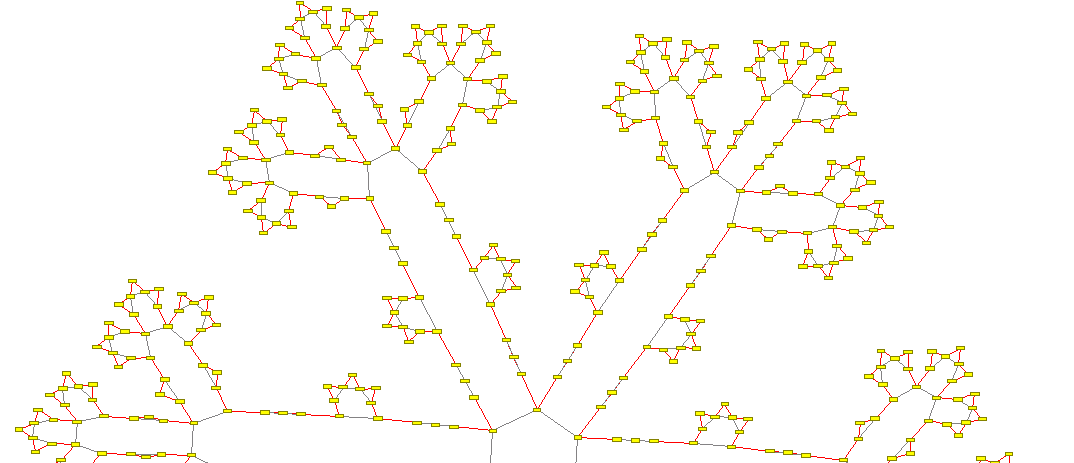
\includegraphics[width=0.9\linewidth]{fig/title}\\[3ex]
  \LARGE Jakob Blomer \qquad Rubino Gei\ss\\[3ex]
  \large \today\\
  
  \vfill
	\large Technical Report 2007-5\\
	\large ISSN 1432-7864	

  \setlength{\parindent}{\saveparindent}
\end{titlepage}
\clearpage

\chapter*{Abstract}
This is the abstract. TODO!

\clearpage

\tableofcontents

\chapter{Introduction}
\pagenumbering{arabic}


\section{What is \GrG?}

{\scshape GrGen} (\textsc{G}raph \textsc{R}ewrite \textsc{Gen}erator) is a generative programming system for graph rewriting.
For the potentially expensive matching problem, {\scshape GrGen} applies several novel heuristic optimizations.
According to \indexed{Varr\'o's benchmark}, it is at least one order of magnitude faster than any other tool known to us.

In order to accelerate the matching step, we internally introduce \newterm{search plans} to represent different \newterm{matching strategies} and equip these search plans with a cost model, taking the present host graph into account.
The task of selecting a good search plan is then considered as an optimization problem~\cite{BKG:07,Bat:06}.
For the rewrite step, our tool implements the well-founded \newterm{single-pushout approach} (SPO, for explanation see~\cite{spoapproach}).

For ease of use, {\scshape GrGen} features an expressive specification language and generates program code with a convenient interface.
In contrast to systems like \indexed{Fujaba}~\cite{fujaba} our pattern matching algorithm is fully automatic and does not need to be tuned or partly be implemented by hand.
\GrG~\cite{grgen_web} is the successor of the \textsc{GrGen} tool presented at ICGT 2006~\cite{GBGHS:06}. 
The ``.NET'' postfix of the new name indicates that \textsc{GrGen} has been reimplemented in C\# for the Microsoft .NET or Mono environment~\cite{NET,MONO}.


\section{Features of \GrG}

The process of graph rewriting can be divided into four steps:
Representing a graph according to a model, searching a pattern aka finding a match, performing changes to the matched spot in the host graph, and, finally, selecting the next rule(s) for application.
We have organized the features of \GrG\ according to this breakdown of graph rewriting.

\begin{itemize}
  \item The graph model (meta-model) supports:
  \begin{itemize}
    \item Directed graphs
    \item Typed nodes and edges, with multiple inheritance on types
    \item Node and edge types can be equipped with typed attributes (like structs)
    \item Multigraphs (including multiple edges of the same type)
    \item Connection assertions to restrict the ``shape'' of graphs
  \end{itemize}
  
  \item The pattern language supports:
  \begin{itemize}
    \item Plain isomorphic subgraph matching (injective mapping)
    \item Homomorphic matching for a selectable set of nodes/edges, so that the matching is not injective
    \item Attribute conditions (including arithmetic operations on the attributes)
    \item Type conditions (including powerful instanceof-like type expressions)
    \item Parameter passing to rules
    \item \indexed{Dynamic patterns} with iterative or recursive paths and graphs (yet to be implemented)
  \end{itemize}
  
  \item The rewrite language supports:
  \begin{itemize}
    \item Attribute re-calculation (using arithmetic operations on the attributes)
    \item Retyping of nodes/edges (a stronger version of casts known from common programming languages)
    \item Creation of new nodes/edges of statically as well as dynamically computed types (some kind of generic templates)
    \item Two modes of specification: A rule can either express changes to be made to the match or replace the whole match (the semantics is always mapped to SPO)
    \item Returning certain edges/nodes for further computations
	  \item Copying (duplicating) of elements form the match---comparable with \indexed{sesqui-pushout} rewriting~\cite{CHHK:06} (yet to be implemented)
  \end{itemize}
  
  \item The rule application language (\GrShell) supports:
  \begin{itemize}
    \item Composing several rules with logical and iterative sequence control (called graph rewrite sequences, GRS)
    \item Various methods for creation/deletion/input/output of graphs/nodes/edges 
    \item Stepwise and graphic debugging of rule application
    \item Graph rewrite sequences that can contain nested transactions\indexmain{transaction, nested}
  \end{itemize}
  
  \item Alternatively to \GrShell, you can access the match and rewrite facility through \LibGr. In this way you can build your own algorithmic rule applications in a .NET language of your choice. 
\end{itemize}


\section{System Overview}

Figure~\ref{figsys} gives an overview of the \GrG\ system components. Table~\ref{dirstruc} shows the \GrG\ directory structure.

\begin{figure}[htbp]
  \centering
	\scalebox{0.8}{
  \begin{tikzpicture}
      \begin{scope}[shape=rectangle,minimum size=0.75cm,text width=3cm,text centered]
          \tikzstyle{every node}=[draw]
          \node (spec1)    at (0   ,0)    {Rewrite Rules\indexmain{rewrite rule} (*\indexed{.grg})};
          \node (spec2)    at (0   ,2)    {Graph Model\indexmain{graph model} (*\indexed{.gm})};
          \node (grgen)    at (4   ,1)    {\GrG\ Generator\indexmain{generator} (Java, C\#)};
          \node (rewriter) at (10  ,0)    {Rewrite~Rules (C\#)};
          \node (types)    at (10  ,2)    {Graph~Model (C\#)};
          \node (data)     at (14  ,1)    {Graph~Management (C\#)};
          \node (libgr)    at (12  ,4)    {\LibGr\indexmain{libGr}\ (C\#)};
          \node[fill,color=gray] (app)      at (14.1  ,5.6)  {};
          \node[fill=white] (app)      at (14  ,5.5)  {Applications};
          \node (grsh)     at (10  ,5.5)  {\GrShell\indexmain{GrShell}\ (C\#)};
          \node (grs)      at (6   ,5.5)  {Graph Rewrite Script\indexmain{graph rewrite script}\indexmainsee{GrShell script}{graph rewrite script}\indexmainsee{script}{graph rewrite script} (*\indexed{.grs})};
      \end{scope}

      \node[draw, minimum width=9cm,minimum height=4cm] (engine) at (12,1) {};
      \node[draw, minimum width=9cm,minimum height=4cm,style=dotted] (ct) at (2,1) {};
      \node[anchor=north east] (engine_lab) at (engine.north east) {Backend\indexmain{backend} (Run Time)};
      \node[anchor=north east] (ct_lab) at (ct.north east) {Frontend (Compile Time)};

      \draw[->,dashed,red,>=triangle 45]     (spec1)   -> (grgen);
      \draw[->,dashed,red,>=triangle 45]     (spec2)   -> (grgen);
      \draw[->,dashed,red,>=triangle 45]     (grgen)   -> (types);
      \draw[->,line width=1pt,>=triangle 45] (grgen)   -> (engine);
      \draw[->,dashed,red,>=triangle 45]     (grgen)   -> (rewriter);
      \draw[->,line width=1pt,>=triangle 45] (app)     -> (libgr);
      \draw[->,line width=1pt,>=triangle 45] (grsh)    -> (libgr);
      \draw[->,dashed,red,>=triangle 45]     (grs)     -> (grsh);
      \draw[->,line width=1pt,>=triangle 45] (libgr)   -> (engine);

      \draw[->,line width=1pt,>=triangle 45] (-1.75,5.5) -- +(2.5,0) node[above, midway] {call};
      \draw[->,dashed,red,>=triangle 45] (-1.75,4.5)  -- +(2.5,0) node[above, midway] {read / generate};
  \end{tikzpicture}
	}
  \caption{\GrG\ system components~\cite{Kro:07}}
  \label{figsys}
\end{figure}
\begin{table}[htbp]
  \begin{tabularx}{\linewidth}{|lX|} \hline
  bin & Contains the .NET assemblies, in particular \indexed{GrGen.exe} (the graph rewrite system generator), \indexed{lgspBackend.dll} (a \GrG\ backend), \indexed{LibGr.dll} (the backend API), and the shell \indexed{GrShell.exe}.  \\ 
  lib & Contains the \GrG\ generated assemblies (*.dll). \\
  specs & Contains the graph rewrite system source documents (*.gm and *.grg). \\ \hline
  \end{tabularx}
  \caption{\GrG\ directory structure}
  \label{dirstruc}
\end{table}

A graph rewrite system\footnote{In this context, system is not a CH0-like grammar rewrite system, but rather a set of interacting software components.} is defined by a rule set file (*.grg) and zero or more graph model description files (*.gm). 
Such a graph rewrite system is generated from these specifications by GrGen.exe and can be used by applications such as \GrShell.
Figure~\ref{process} shows the generation process.

\begin{figure}[htbp]
  \centering
	\scalebox{0.8}{
  \begin{tikzpicture}
      \begin{scope}[shape=rectangle,minimum size=0.75cm,text width=3cm,text centered]
          \tikzstyle{every node}=[draw]
          \node (gm1)      at (0   ,0)    {model1.gm};
          \node (gm2)      at (0   ,1)    {model2.gm};
          \node (gm3)      at (0   ,2)    {model3.gm};
          \node (grg)      at (4.5 ,1)    {rules1.grg};
          \node (grgen)    at (10   ,1)    {GrGen.exe};
          \node (act)      at (15.5,1) {rules1Actions.dll};
          \node (backend)  at (10   ,2)    {backend.dll};
          \node (mod)      at (15.5,2)  {rules1Model.dll};
      \end{scope}
         
			\draw[|-|] (-1,-1.5)   -- (5.5, -1.5)    node[below, midway] {/specs};
			\draw[|-|] (9,-1.5)    -- (11, -1.5)     node[below, midway] {/bin};
			\draw[|-|] (14.5,-1.5) -- (16.5, -1.5)   node[below, midway] {/lib};

      \draw[->,line width=1pt,>=triangle 45]     (grg)     -> (gm1);
      \draw[->,line width=1pt,>=triangle 45]     (grg)     -> (gm2);
      \draw[->,line width=1pt,>=triangle 45]     (grg)     -> (gm3);
      \draw[->,dashed,red,>=triangle 45]         (grg)     -> (grgen);
      \draw[->,dashed,red,>=triangle 45]         (grgen)   -> (mod);
      \draw[->,dashed,red,>=triangle 45]         (grgen)   -> (act);
      \draw[->,line width=1pt,>=triangle 45]     (mod)     -> (backend);
      \draw[->,line width=1pt,>=triangle 45]     (act)     -> (backend);


      \draw[->,line width=1pt,>=triangle 45] (-1.25,3.5) -- +(2.5,0) node[above, midway] {referencing};
      \draw[->,dashed,red,>=triangle 45]     (3.25,3.5)  -- +(2.5,0) node[above, midway] {read / generate};
  \end{tikzpicture}
	}
  \caption{Generating a graph rewrite system}
  \label{process}
\end{figure}

In general you have to distinguish carefully between a graph model (meta level), a host graph, a pattern graph and a rewrite rule.
In \GrG\ pattern graphs are implicitly defined by rules, i.e.\ each rule defines its pattern.
On the technical side, specification documents for a graph rewrite system can be available as source documents for graph models and rule sets (plain text *.gm and *.grg files) or as their translated .NET modules, either C\# source files or their compiled assemblies (*.dll).

Generating a \GrG\ graph rewrite system may be considered as preliminary task.
The actual process of rewriting as well as dealing with host graphs is performed by \GrG's backend.
\GrG\ provides a backend \indexed{API}---the .NET library \LibGr.
For most issues---in particular for experimental purposes---you might rather want to work with the \GrShell\ because of its more convenient interface.
However, \GrShell\ does not provide the full power of the \LibGr; see also note~\ref{note:indeterminism} on page~\pageref{note:indeterminism}.

\section{What is Graph Rewriting?}
\label{ov:whatsallabout}

The notion of graph rewriting as understood by \GrG\ is a method for declaratively specifying ``changes'' to a graph.
This is comparable to the well-known term rewriting. 
Normally you use one or more \newterm{graph rewrite rules} to accomplish a certain task.
\GrG\ implements an SPO-based approach.
In the simplest case such a graph rewrite rule consists of a tuple $L \rightarrow R$, whereas $L$---the \newterm{left hand side}\indexmainsee{LHS}{left hand side} of the rule---is called \newterm{pattern graph} and $R$---the \newterm{right hand side}\indexmainsee{RHS}{right hand side} of the rule---is the \newterm{replacement graph}.

\begin{figure}[htbp]
	\centering
  \begin{tikzpicture}
    \begin{scope}[minimum size=0.5cm]
      \tikzstyle{every node}=[draw]
      \node (L)     at (0   ,2.5) {$L$};
      \node (R)     at (7   ,2.5) {$R$};
      \node (mL)    at (0   ,0) {};
      \node (mR)    at (7   ,0) {};
      \node[text width=2cm,text badly ragged,minimum size=1cm] (H)     at (0   ,0) {$H$};
      \node[text width=2cm,text badly ragged,minimum size=1cm] (Hs)    at (7   ,0) {$H'$};
    \end{scope}

    \draw[dotted,->] (L) node[above=0.4cm] {Pattern Graph} -> (mL) node[left,midway]  {Match $m$}   node[below=0.6cm] {Host Graph};
    \draw[dotted,->] (R) node[above=0.4cm] {Rewrite Graph} -> (mR)                              node[below=0.6cm] {Result Graph};

    \pgfsetshortenstart{0.5cm}
    \pgfsetshortenend{0.5cm}
    \draw[thick,->]  (L) -> (R)  node[above,midway] {Preservation Morphism $r$} node[below,midway] {Rule};
    \draw[thick,->]  (H) -> (Hs) node[below,midway] {Rule Application};
  \end{tikzpicture}
  \caption{Basic Idea of Graph Rewriting}
  \label{figrule}
\end{figure}

Moreover we need to identify graph elements (nodes or edges) of $L$ and $R$ for preserving them during rewrite. 
This is done by a \newterm{preservation morphism} $r$ mapping elements from $L$ to $R$; the morphism $r$ is injective, but needs to be neither surjective nor total.
Together with a rule name $p$ we have $p : L \xrightarrow{r} R$.

The transformation is done by \newterm{application}\indexmainsee{rule application}{application} of a rule to a \newterm{host graph} $H$.
To do so, we have to find an occurrence of the pattern graph in the host graph. 
Mathematically speaking, such a \newterm{match} $m$ is an isomorphism from $L$ to a subgraph of $H$.
This morphism may not be unique, i.e.\ there may be several matches.
Afterwards we change the matched \indexed{spot} $m(L)$ of the host graph, such that it becomes an isomorphic subgraph of the replacement graph $R$.
Elements of $L$ not mapped by $r$ are deleted from $m(L)$ during rewrite.
Elements of $R$ not in the image of $r$ are inserted into $H$, all others (elements that are mapped by $r$) are retained.
The outcome of these steps is the resulting graph $H'$. In symbolic language: $H \xRightarrow{m, p} H'$.


\section{An Example}
\label{ov:example}

We'll have a look at a small example. 
Graph elements (nodes and edges) are labeled with and identifier.
If a type is necessary then it is stated after a colon.
We start using a special case to construct our host graph: an \indexed{empty pattern} always produces exactly one\footnote{Because of the uniqueness of the total and totally undefined morphism.} match (independent of the host graph). So we construct an apple by applying
\[
  p_0:  
  \begin{array}[c]{c} 
    \emptyset
  \end{array} 
  \begin{array}[c]{c} 
    \longrightarrow 
  \end{array} 
  \begin{array}[c]{c} 
    \begin{tikzpicture}[show background rectangle]
      \tikzstyle{every node}=[circle]
      \node[draw] (n1) at (2.5,5) {};
      \node[draw] (n2) at (2,4)   {};
      \node[draw] (n3) at (0,2)   {};
      \node[draw] (n4) at (2,0)   {};
      \node[draw] (n5) at (4,2)   {};
    	
    	\draw[-latex] (n2) --                                  (n1) node[left,midway]  {$e_1$};
    	\draw[-latex] (n2) .. controls +(-1,1) and +(0,1) ..   (n3) node[left,midway]  {$e_2$};
      \draw[-latex] (n3) .. controls +(0,-1) and +(-1,0) ..  (n4) node[left,midway]  {$e_3$};
    	\draw[-latex] (n4) .. controls +(1,0)  and +(0,-1) ..  (n5) node[right,midway] {$e_4$};
      \draw[-latex] (n5) .. controls +(0,1)  and +(1,1) ..   (n2) node[right,midway] {$e_5$};
    \end{tikzpicture}
  \end{array}
\]
to the empty host graph. 
As the result we get an apple as new host graph $H$. 
Now we want to rewrite our apple with stem to an apple with a leaflet. 
So we apply
\[
  p_1:
  \begin{array}[c]{c}
    \begin{tikzpicture}[show background rectangle]
      \tikzstyle{every node}=[circle,minimum size=0.7cm]
      \node[draw] (a) at (2,5.5)  {a};
      \node[draw] (b) at (2,4)    {b};
    	
    	\draw[-latex] (b) -- (a) node[left,midway]  {$x$};
    \end{tikzpicture}
  \end{array}
  \begin{array}[c]{c}
    \longrightarrow
  \end{array}
  \begin{array}[c]{c}
    \begin{tikzpicture}[show background rectangle]
      \tikzstyle{every node}=[circle,minimum size=0.7cm]
      \node[draw] (c) at (2,5.5)  {c};
      \node[draw] (b) at (2,4)    {b};
    	
    	\draw[-latex] (b) .. controls +(-0.7,+0.7) and +(-0.7,-0.7) .. (c) node[left,midway]   {$y$};
    	\draw[-latex] (b) .. controls +(+0.7,+0.7) and +(+0.7,-0.7) .. (c) node[right,midway]  {$z$};
    \end{tikzpicture}
  \end{array} 
\]
to $H$ and get the new host graph $H_1$, something like this:
\[
  \begin{array}[c]{c} 
    \begin{tikzpicture}[show background rectangle]
      \tikzstyle{every node}=[circle]
      \node[draw] (n1) at (2.5,5) {};
      \node[draw] (n2) at (2,4)   {};
      \node[draw] (n3) at (0,2)   {};
      \node[draw] (n4) at (2,0)   {};
      \node[draw] (n5) at (4,2)   {};
    	
    	\draw[-latex] (n2) --                                  (n1) node[left,midway]  {$e_1$};
    	\draw[-latex] (n2) .. controls +(-1,1) and +(0,1) ..   (n3) node[left,midway]  {$e_2$};
      \draw[-latex] (n3) .. controls +(0,-1) and +(-1,0) ..  (n4) node[left,midway]  {$e_3$};
    	\draw[-latex] (n4) .. controls +(1,0)  and +(0,-1) ..  (n5) node[right,midway] {$e_4$};
      \draw[-latex] (n5) .. controls +(0,1)  and +(1,1) ..   (n2) node[right,midway] {$e_5$};
    \end{tikzpicture}
  \end{array} 
  \begin{array}[c]{c} 
    \xRightarrow{\quad p_1 \quad}
  \end{array} 
  \begin{array}[c]{c} 
    \begin{tikzpicture}[show background rectangle]
      \tikzstyle{every node}=[circle]
      \node[draw] (n1) at (2.5,5) {};
      \node[draw] (n2) at (2,4)   {};
      \node[draw] (n3) at (0,2)   {};
      \node[draw] (n4) at (2,0)   {};
      \node[draw] (n5) at (4,2)   {};
      \node[draw] (n6) at (0,0.5)   {};
    	
    	\draw[-latex] (n2) --                                  (n1) node[left,midway]  {$e_1$};
    	\draw[-latex] (n2) .. controls +(-1,1) and +(0,1) ..   (n3) node[left,midway]  {$e_2$};
      \draw[-latex] (n3) .. controls +(-0.7,-0.7) and +(-0.7,+0.7) .. (n6) node[left,midway]  {$e_6$};
      \draw[-latex] (n3) .. controls +(+0.7,-0.7) and +(+0.7,+0.7) .. (n6) node[right,midway] {$e_7$};
    	\draw[-latex] (n4) .. controls +(1,0)  and +(0,-1) ..  (n5) node[right,midway] {$e_4$};
      \draw[-latex] (n5) .. controls +(0,1)  and +(1,1) ..   (n2) node[right,midway] {$e_5$};
    \end{tikzpicture}
  \end{array}
\]
What happened? 
\GrG\ has arbitrarily chosen one match out of the set of possible matches, because $x$ matches edge $e_3$ as well as $e_1$.
A correct solution could make use of edge type information. 
We have to change rule $p_0$ to generate the edge $e_1$ with a special type ``stem''.
And this time we will even keep the stem. 
So let
\[
  p_2:
  \begin{array}[c]{c}
    \begin{tikzpicture}[show background rectangle]
      \tikzstyle{every node}=[circle,minimum size=0.7cm]
      \node[draw] (a) at (2,5.5)  {a};
      \node[draw] (b) at (2,4)    {b};
    	
    	\draw[-latex] (b) -- (a) node[left,midway]  {$x:\text{stem}$};
    \end{tikzpicture}
  \end{array}
  \begin{array}[c]{c}
    \longrightarrow
  \end{array}
  \begin{array}[c]{c}
    \begin{tikzpicture}[show background rectangle]
      \tikzstyle{every node}=[circle,minimum size=0.7cm]
      \node[draw] (c) at (2,5.5)  {c};
      \node[draw] (b) at (2,4)    {b};
      \node[draw] (a) at (3.5,5.5){a};
    	
    	\draw[-latex] (b) -- (a) node[right,midway]  {$x$};
    	\draw[-latex] (b) .. controls +(-0.7,+0.7) and +(-0.7,-0.7) .. (c) node[left,midway]   {$y$};
    	\draw[-latex] (b) .. controls +(+0.7,+0.7) and +(+0.7,-0.7) .. (c) node[above,midway]  {$z$};
    \end{tikzpicture}
  \end{array}.
\]
If we apply $p_2$ to the modified $H_1$ this leads to
\[
  \begin{array}[c]{c} 
    \begin{tikzpicture}[show background rectangle]
      \tikzstyle{every node}=[circle]
      \node[draw] (n1) at (2.5,5) {};
      \node[draw] (n2) at (2,4)   {};
      \node[draw] (n3) at (0,2)   {};
      \node[draw] (n4) at (2,0)   {};
      \node[draw] (n5) at (4,2)   {};
    	
    	\draw[-latex] (n2) --                                  (n1) node[left,pos=0.8]  {$e_1:\text{stem}$};
    	\draw[-latex] (n2) .. controls +(-1,1) and +(0,1) ..   (n3) node[left,midway]  {$e_2$};
      \draw[-latex] (n3) .. controls +(0,-1) and +(-1,0) ..  (n4) node[left,midway]  {$e_3$};
    	\draw[-latex] (n4) .. controls +(1,0)  and +(0,-1) ..  (n5) node[right,midway] {$e_4$};
      \draw[-latex] (n5) .. controls +(0,1)  and +(1,1) ..   (n2) node[right,midway] {$e_5$};
    \end{tikzpicture}
  \end{array} 
  \begin{array}[c]{c} 
    \xRightarrow{\quad p_2 \quad}
  \end{array} 
  \begin{array}[c]{c} 
    \begin{tikzpicture}[show background rectangle]
      \tikzstyle{every node}=[circle]
      \node[draw] (n1) at (3,5) {};
      \node[draw] (n2) at (2,4)   {};
      \node[draw] (n3) at (0,2)   {};
      \node[draw] (n4) at (2,0)   {};
      \node[draw] (n5) at (4,2)   {};
      \node[draw] (n6) at (2,5.0)   {};
    	
    	\draw[-latex] (n2) --                                  (n1) node[right,pos=0.6] {$e_1:\text{stem}$};
    	\draw[-latex] (n2) .. controls +(-1,1) and +(0,1) ..   (n3) node[left,midway]  {$e_2$};
      \draw[-latex] (n3) .. controls +(0,-1) and +(-1,0) ..  (n4) node[left,midway]  {$e_3$};
    	\draw[-latex] (n4) .. controls +(1,0)  and +(0,-1) ..  (n5) node[right,midway] {$e_4$};
      \draw[-latex] (n5) .. controls +(0,1)  and +(1,1) ..   (n2) node[right,midway] {$e_5$};
    	\draw[-latex] (n2) .. controls +(-0.3,+0.3) and +(-0.3,-0.3) .. (n6) node[left,midway]   {};
    	\draw[-latex] (n2) .. controls +(+0.3,+0.3) and +(+0.3,-0.3) .. (n6) node[right,midway]  {};
    \end{tikzpicture}
  \end{array}.
\]

\section{The Tools}

All the programs and libraries of \GrG\ are licensed under \indexed{LGPL}. Notice that the \yComp\ graph viewer is not a part of \GrG ; \yComp\ ships with its own license. Although \yComp\ is not free software, it's free for use in academic and non-commercial areas.

\subsection{\texttt{\indexed{GrGen.exe}}}
The \texttt{GrGen.exe} assembly implements the \GrG\ generator. The \GrG\ generator parses a rule set and its model files and compiles them into .NET assemblies. The compiled assemblies interact with the \GrG\ backend.
\begin{description}
  \item[Usage] \texttt{[mono] GrGen.exe [-use <existing-dir>] [-keep] <rule-set> [<output-dir>]}\\
    \emph{rule-set} is a file containing a rule set specification according to chapter~\ref{chaprulelang}. Usually such a file has the suffix \texttt{\indexed{.grg}}. The suffix \texttt{.grg} may be omitted.
By default \GrG\ tries to write the compiled assemblies to the directory \texttt{../lib} relative to the path of \texttt{GrGen.exe}. This can be changed by the optional parameter \emph{output-dir}.
  \item[Options] \mbox{} 
    \begin{tabularx}{\linewidth}{lX}
      \texttt{-keep} & Keep the generated C\# source files. A subdirectory \texttt{tmpgrgen$n$}\footnote{$n$ is an increasing number.} within the current directory will be created. This directory contains:
\begin{itemize}
  \item \texttt{printOutput.txt}---a snapshot of \texttt{stdout} during program execution.
  \item \emph{Name}\texttt{Actions.cs}---the C\# source file of the \emph{rule-set}\texttt{Actions.dll} assembly.
  \item \emph{Name}\texttt{Model.cs}---the C\# source file(s) of the \emph{rule-set}\texttt{Modell.dll} assembly.
\end{itemize}\\
      \texttt{-use} & Don't re-generate C\# source files. Instead use the files in \emph{existing-dir} to build the assemblies.	
    \end{tabularx}
  \item[Requires] .NET 2.0 (or above) or Mono 1.2.2 (or above). Java Runtime Environment 1.5 (or above).
\end{description}

\subsection{\texttt{\indexed{GrShell.exe}}}
The \GrShell\indexmain{GrShell} is a shell application of the \LibGr. \GrShell\ is capable of creating, manipulating, and dumping graphs as well as performing graph rewriting with graphical debug support. For further information about the \GrShell\ language see chapter~\ref{chapgrshell}.

\begin{description}
  \item[Usage] \texttt{[mono] grShell.exe [-c "<commands>" | <grshell-script>]}\\
     Opens the interactive shell. The \GrShell\ will execute the commands in \emph{grshell-script}\indexmain{graph rewrite script} (usually a \texttt{*\indexed{.grs}} file) immediately.  
  \item[Options] \mbox{} 
    \begin{tabularx}{\linewidth}{lX}
      \texttt{-c} & Execute the quoted \GrShell\ commands immediately. Instead of a line break use a double semicolon \texttt{;;} to separate commands.
    \end{tabularx}
  \item[Requires] .NET 2.0 (or above) or Mono 1.2.2 (or above).
\end{description}

\subsection{\texttt{\indexed{LibGr.dll}}}
The \LibGr\indexmain{libGr} is a .NET assembly implementing \GrG's \indexed{API}. See the extracted HTML documentation for interface descriptions. 

\subsection{\texttt{\indexed{yComp.jar}}}
\label{tools:ycomp}
\yComp\indexmain{yComp} \cite{ycomp} is a graph visualization tool based on \yFiles\ \cite{yfiles}. 
It is well integrated in \GrG, but it's not a part of \GrG. \yComp\ implements several graph layout algorithms and has file format support for \indexed{VCG}, GML and YGF among others. 
\begin{description}
  \item[Usage] Usually \yComp\ will be loaded by the \GrShell. You might want to open \yComp\ manually by typing\\
   \texttt{java -jar yComp.jar [<graph-file>]}\\
  The \emph{graph-file} may be any graph file in a supported format. \yComp\ will open this file on startup.
  \item[Hints] Do not use the \indexedsee{compiler graph}{layout algorithm} \indexed{layout algorithm} (\yComp's default setting). 
  Instead \texttt{\indexedsee{Organic}{layout algorithm}} or \texttt{\indexedsee{Orthogonal}{layout algorithm}} might be good choices. 
  Use the rightmost blue play button to start layout process. This may take a while, depending on the graph size:
\begin{center}
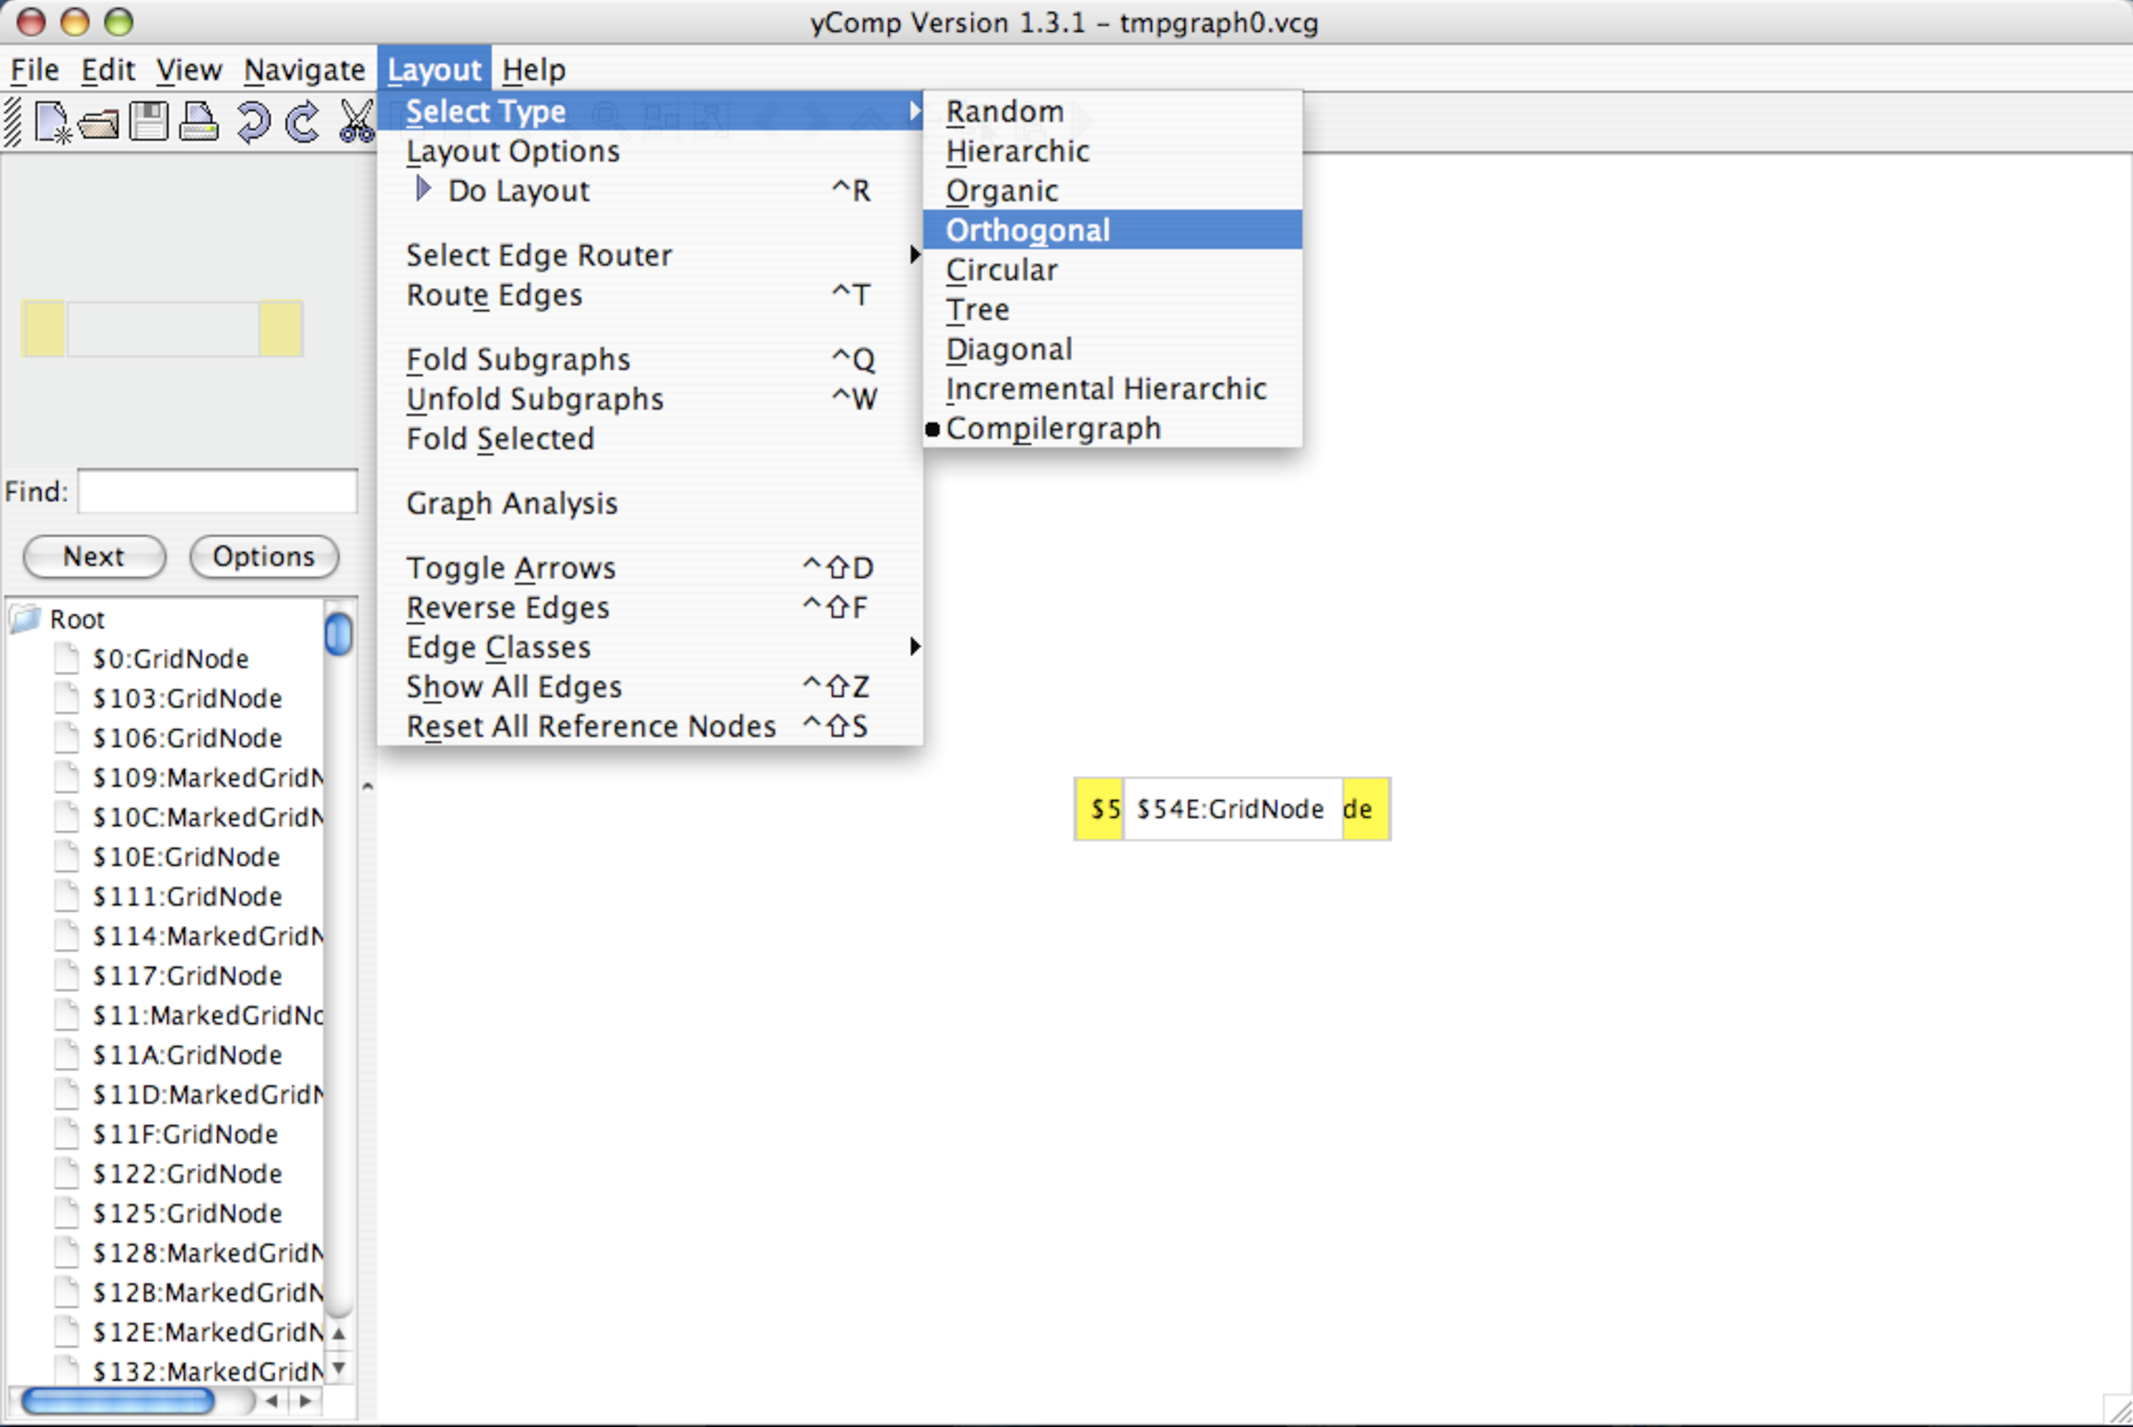
\includegraphics[width=0.45\linewidth]{fig/ycomp1.pdf} 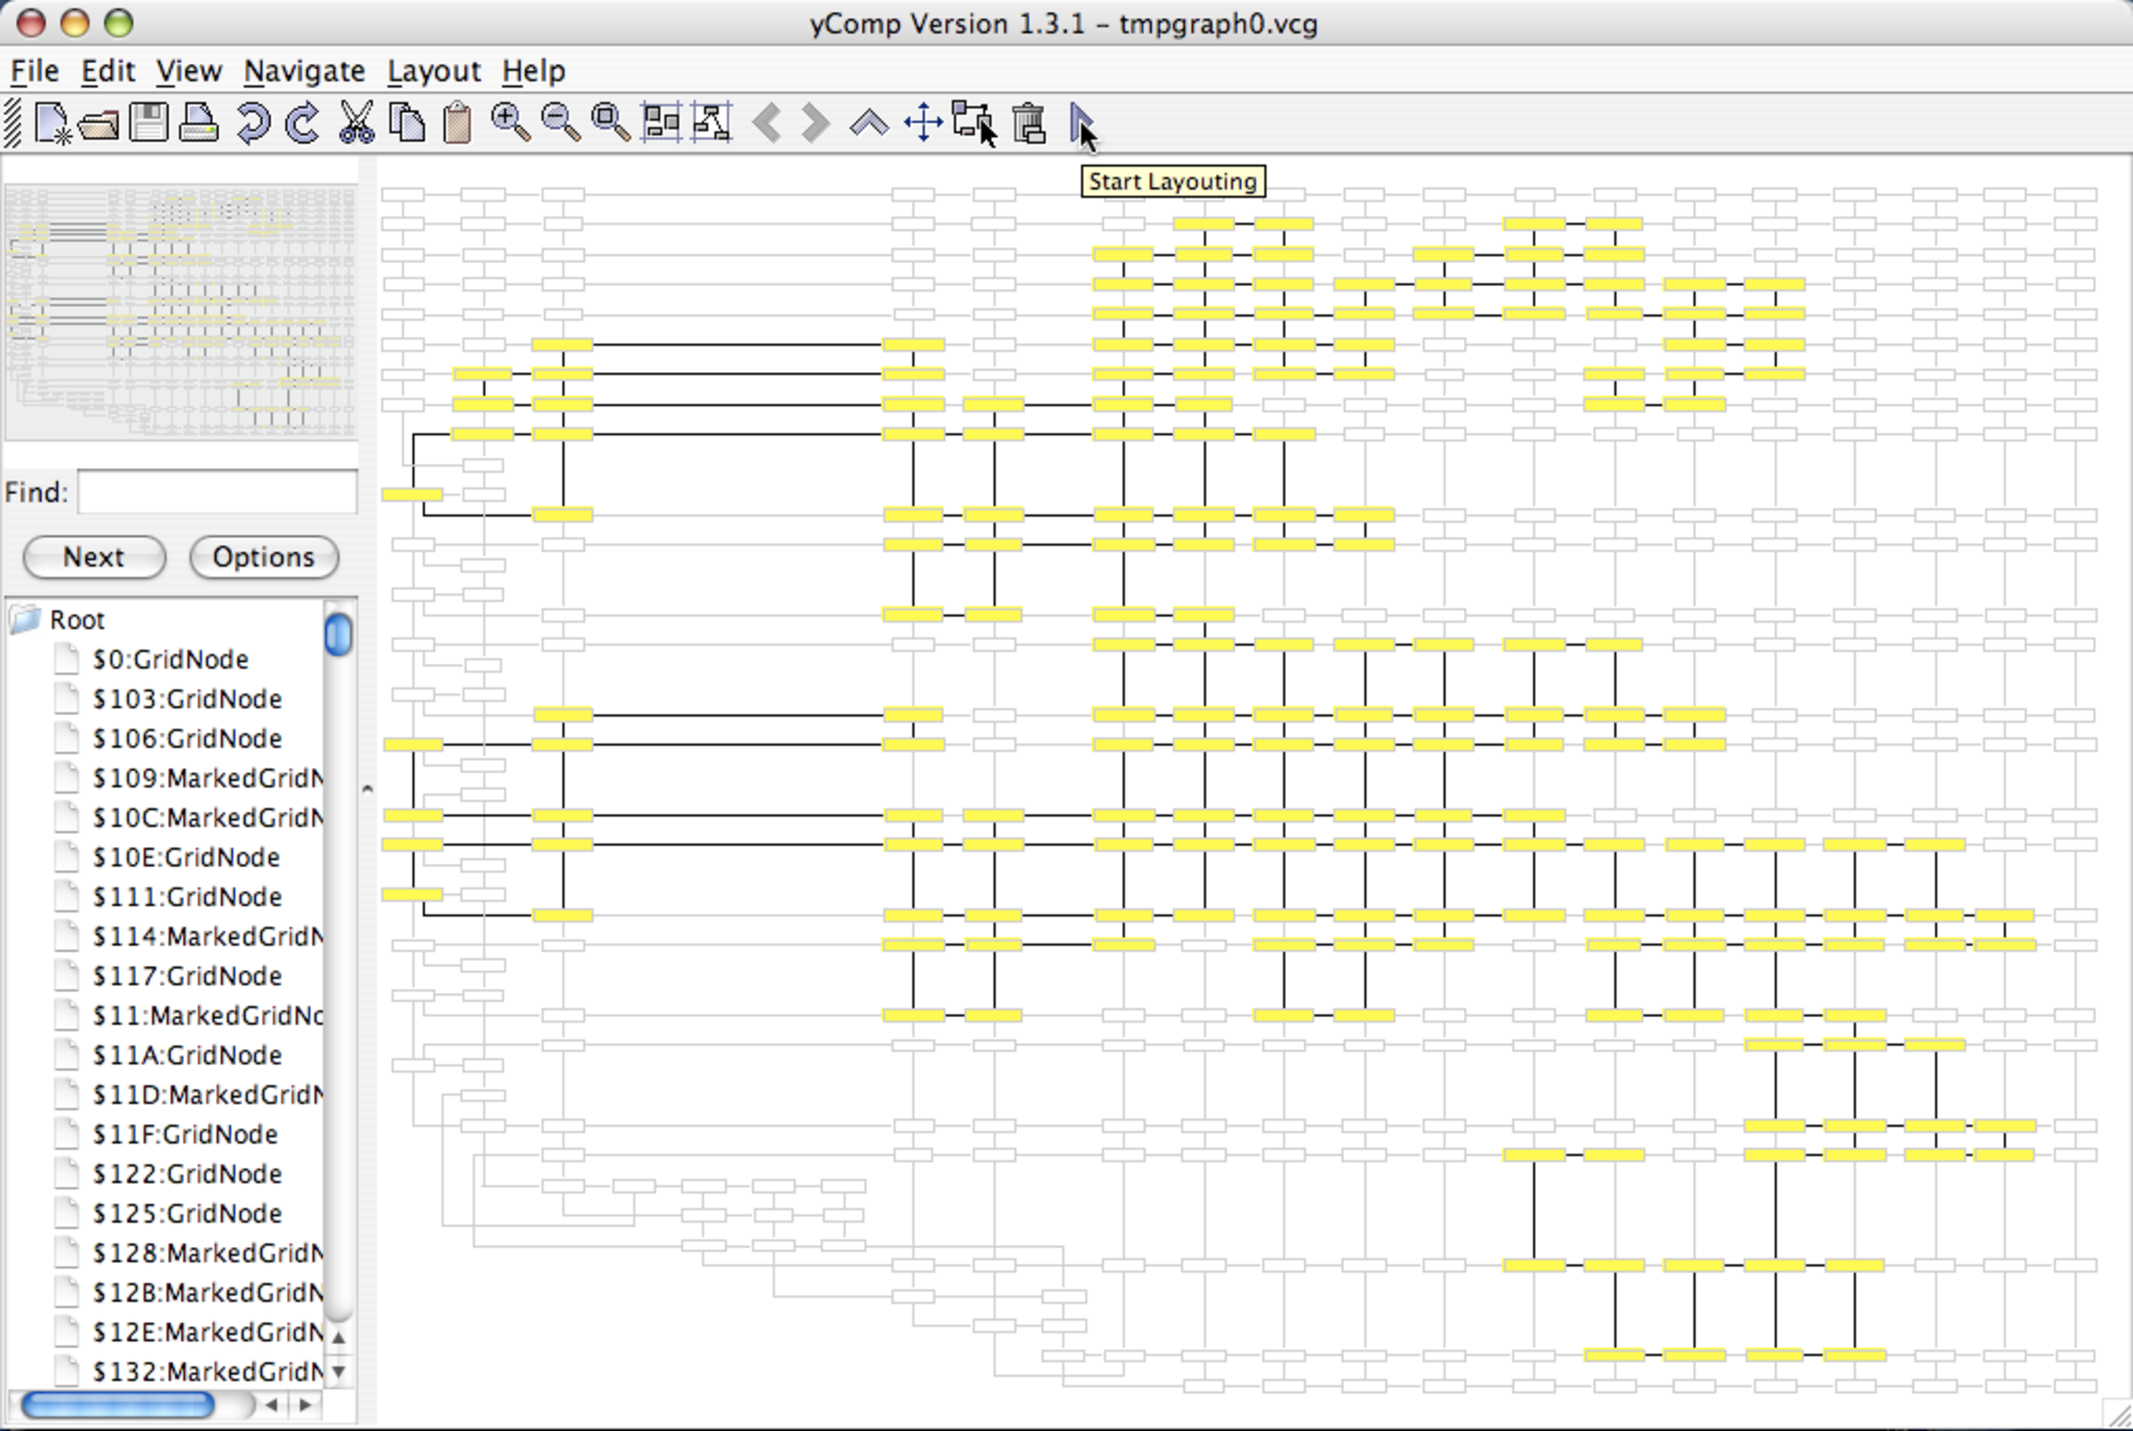
\includegraphics[width=0.45\linewidth]{fig/ycomp2.pdf}
\end{center}
  \item[Requires] Java Runtime Environment 1.5 (or above).
\end{description}




\chapter{Graph Model Language}\indexmain{graph model language}
\label{chapmodellang}
The key features of \GrG\ \emph{graph models}\indexmain{graph model} as described by Geiß et al. \cite{GBGHS:06,KG:07}:

\begin{description}
\item[Types] Nodes and edges are typed. 
  This is similar to classes in common programming languages, except for the concept of methods that \GrG\ nodes and edges don't support. 
\item[Attributes] Nodes and edges can possess attributes. The set of attributes assigned to a node or edge is determined by its type. The attributes themselves are typed, too.
\item[Inheritance] Node and edge types (classes) can be composed by multiple \indexed{inheritance}. \texttt{Node} and \texttt{Edge} are built-in root types of node and edge types, respectively. Inheritance eases the specification of attributes because subtypes inherit the attributes of their super types. Note that \GrG\ lacks a concept of overwriting. On a path in the \indexed{type hierarchy} graph from a type up to the built-in root type there must be exactly one declaration for each attribute identifier. Furthermore if multiple paths from a type up to the built-in root type exist, the declaring types for an attribute identifier must be the same on all such paths.
\item[Connection Assertions] To specify that certain edge types should only connect specific nodes, we include connection assertions. Furthermore the number of outgoing and incoming edges can be constrained.
\end{description}

\begin{figure}[htbf]
\begin{example}\label{ex:model:map}
The following toy example of a model of road maps gives a rough picture of the language:
\begin{grgen}
model Map;

enum resident {village = 500, town = 5000, city = 50000}

node class sight;

node class city {
	size: resident;
}

const node class metropolis extends city {
  river: string;
}  

abstract node class abandoned_city extends city;
node class ghost_town extends abandoned_city;

edge class street;
edge class trail extends street;
edge class highway extends street
    connect metropolis [+] -> metropolis [+]
{
    jam: boolean;
}
\end{grgen}
\end{example}
\end{figure}
In this chapter as well as in chapter \ref{chapgrshell} (\GrShell) we use excerpts of example~\ref{ex:model:map} (the \texttt{Map} model) for illustration purposes.

\section{Building Blocks}
\label{modelbb}

\begin{note}
The following syntax specifications make heavy use of \newtermsee{syntax diagram}{rail diagram}s (also known as \indexed{rail diagram}s). Syntax diagrams provide a visualization of EBNF\footnote{Extended Backus–Naur Form.} grammars. Follow a path along the arrows through a diagram to get a valid sentence (or sub sentence) of the language. Ellipses represent terminals whereas rectangles represent non-terminals. For further information on syntax diagrams see \cite{MMJW:91}.
\end{note}
Basic elements of the \GrG\ graph model language are identifiers to denominate types, attributes, and the model itself. The \GrG\ graph model language is \indexed{case sensitive}.\\
\\
\emph{Ident}, \emph{IdentDecl}\\ \indexmain{identifier}\nopagebreak
A non-empty character sequence of arbitrary length consisting of letters, digits, or underscores. The first character must not be a digit. \emph{Ident} and \emph{IdentDecl} differ in their role: While \emph{IdentDecl} is a \emph{defining} occurrence of an identifier, \emph{Ident} is a \emph{using} occurrence. An \emph{IdentDecl} non-terminal can be annotated\indexmain{annotation}. See \ref{annotations} for annotations of declarations.
\begin{note}
\label{note:modeldecl}
  The \GrG\ model language does not distinguish between \indexed{declaration}s and \indexed{definition}s. More precisely, every declaration is also a definition. For instance, the following C-like pseudo \GrG\ model language code is illegal:
\begin{grgen}
node class t_node;
node class t_node {
  ...
}
\end{grgen}
Using an identifier before defining it is allowed. Every used identifier has to be defined exactly once.
\end{note}
\mbox{ }\\
\emph{NodeType}, \emph{EdgeType}, \emph{EnumType}\\ \nopagebreak
These are (semantic) specializations of \emph{Ident} to restrict an identifier to denote a node type, an edge type, or an enum type, respectively.

\section{Type Declarations}
\begin{rail}
  GraphModel: 'model' IdentDecl ';' (() + TypeDeclaration);
\end{rail}\ixkeyw{model}\ixnterm{GraphModel}
The \indexed{graph model} consists of its name \emph{IdentDecl} and type declarations defining specific node and edge types as well as enums.

\begin{rail}
  TypeDeclaration: EnumDeclaration | ClassDeclaration
\end{rail}\ixnterm{TypeDeclaration}
\emph{ClassDeclaration} defines a node type or an edge type. \emph{EnumDeclaration} defines an enum type for use as attribute of nodes or edges. Like all identifier definitions, types do not need to be declared\indexmain{declaration} before they are used.

\begin{rail}
  EnumDeclaration: 'enum' IdentDecl lbrace ((IdentDecl (() | '=' IntExpr)) + ',') rbrace ;
\end{rail}\ixkeyw{enum}\ixnterm{EnumDeclaration}
Defines an \indexed{enum type}.

\begin{example}
\begin{grgen}
enum Color {red, green, blue}
enum Resident {village = 500, town = 5000, city = 50000}
enum AsInC {a = 2, b, c = 1, d, e = (int)Resident::village + c}
\end{grgen}
The semantics is as in C \cite{Sch:1990:ANSIC}. So, the following holds: $\texttt{red} = 0$, $\texttt{green} = 1$, $\texttt{blue} = 2$, $\texttt{a}=2$, $\texttt{b}=3$, $\texttt{c}=1$, $\texttt{d}=2$, and $\texttt{e}=501$.
\end{example}

\begin{rail}  
  ClassDeclaration: (() | 'abstract') (() | 'const') (NodeClass | EdgeClass);
\end{rail}\ixkeyw{abstract}\ixkeyw{const}\ixnterm{ClassDeclaration}
Defines a new node type or edge type. The keyword \texttt{abstract} indicates that you cannot instantiate graph elements of this type. Instead you have to derive non-abstract types to create graph elements. The abstract-property will not be inherited by subclasses, of course.

\begin{example}
We adjust our map model and make \texttt{city} abstract:
\begin{grgen}
abstract node class city {
	size: int;
}
abstract node class abandoned_city extends city;
node class ghost_town extends abandoned_city;
\end{grgen}
You will be able to create nodes of type \texttt{ghost\_town}, but not of type \texttt{city} or \texttt{abandoned\_city}. However, nodes of type \texttt{ghost\_town} are also of type \texttt{abandoned\_city} as well as of type \texttt{city} and they have the attribute \texttt{size}, hence.
\end{example}
The keyword \texttt{const} indicates that rules may not write to attributes (see also section \ref{replacepart}, \texttt{eval}). However, such attributes are still writable by \LibGr\indexmain{libGr} and \GrShell\indexmain{GrShell} directly. This property applies to attributes defined in the current class, only. It does not apply to inherited attributes. The \texttt{const} property will not be inherited by subclasses, either. If you want a subclass to have the \texttt{const} property, you have to set the \texttt{const} modifier explicitly.

\begin{rail}  
  NodeClass: 'node' 'class' IdentDecl (() | 'extends' (NodeType+',')) \\ 
    (';' | lbrace AttributeDeclarations rbrace);
\end{rail}\ixkeyw{node}\ixkeyw{class}\ixkeyw{extends}\ixnterm{NodeClass}
Defines a new \indexed{node type}. Node types can inherit\indexmain{inheritance} from other node types defined within the same file. If the \texttt{extends} clause is omitted, \emph{NodeType} will inherit from the built-in type \texttt{\indexed{Node}}. Optionally nodes can possess attributes.

\begin{rail}    
  EdgeClass: 'edge' 'class' IdentDecl (() | 'extends' (EdgeType+',')) \\
    (() + ConnectAssertions) (';' | lbrace AttributeDeclarations rbrace);
\end{rail}\ixkeyw{edge}\ixkeyw{class}\ixkeyw{extends}\ixnterm{EdgeClass}
Defines a new \indexed{edge type}. Edge types can inherit\indexmain{inheritance} from other edge types defined within the same file. If the \texttt{extends} clause is omitted, \emph{EdgeType} will inherit from the built-in type \texttt{\indexed{Edge}}. Optionally edges can possess attributes. A \newterm{connection assertion} specifies that certain edge types should only connect specific nodes and, moreover, the number of outgoing and incoming edges can be constrained.

\begin{note}
It is not forbidden to create graphs that are invalid according to \indexed{connection assertion}s. \GrG\ just enables you to check, whether a graph is valid or not. See also section \ref{graphcommands}, \texttt{validate}.
\end{note}

\begin{rail}  
  ConnectAssertions: 'connect' (NodeConstraint '->' NodeConstraint + ',');
  NodeConstraint: NodeType (() | '[' ('*' | '+' | Number | RangeConstraint) ']') ;
  RangeConstraint: Number ':' ('*' | Number) ;
\end{rail}\ixkeyw{connect}\ixnterm{ConnectAssertions}\ixnterm{NodeConstraint}\ixnterm{RangeConstraint}
A \indexed{connection assertion} is denoted as a pair of node types in conjunction with their multiplicities\indexmainsee{multiplicity}{connection assertion}. A corresponding edge may connect a node of the first node type or one of its subtypes (source) with a node of the second node type or one of its subtypes (target). The multiplicity is a constraint on the out-degree and in-degree\indexmainsee{degree}{connection assertion} of the source and target node type, respectively. \emph{Number} is an \texttt{int} constant as defined in section \ref{expressions}. See \ref{graphcommands}, \texttt{validate}\ixkeyw{validate}, for an example. Table \ref{multiplicities} describes the multiplicity definitions.
\begin{table}[htbp]
\begin{tabularx}{\linewidth}{|l|X|}\hline
	\texttt{[$n$:*]} & The number of edges, nodes of that type are incident to, is unbounded. At least $n$ edges must be incident to nodes of that type.\\ 
	\texttt{[$n$:$m$]} & At least $n$ edges must be incident to nodes of that type, but at most $m$ edges may be incident to nodes of that type ($m \geq n$ must hold).\\
	\texttt{[*]} & Abbreviation for \texttt{[0:*]}.\\
	\texttt{[+]} & Abbreviation for \texttt{[1:*]}.\\
	\texttt{[$n$]} & Abbreviation for \texttt{[$n$:$n$]}. \\ \hline
\end{tabularx}
\caption{\GrG\ node constraint multiplicities}
\label{multiplicities}
\end{table}

\begin{rail}    
  AttributeDeclarations: (() | IdentDecl ':' AttributeType ';') + ;
  AttributeType: PrimitiveType | EnumType ; 
\end{rail}\ixnterm{AttributeDeclarations}\ixnterm{AttributeType}
Defines a node or edge \indexed{attribute}. Possible types are enumeration types (\texttt{enum}) and primitive types. See section~\ref{builtin} for a list of built-in primitive types.





\chapter{Rule Set Language}
\label{chaprulelang}

The rule set language forms the core of \GrG. Rule files refer to zero\footnote{Omitting a graph model means that \GrG\ uses a default graph meta model. The default model consists of the base type \texttt{Node} for vertices and the base type \texttt{Edge} for edges.} or more graph models and specify a set of rewrite rules. The rule language covers the pattern specification and the replace/modify specification. Attributes of graph elements can be re-evaluated during a rule application. The following rewrite rule by Geiß et al. \cite{geiss} gives a rough picture of the language:
%\begin{figure}[tb]
\begin{example}\label{ex:rule:SomeRule}
\begin{grgen}
actions SomeActions using SomeModel;

rule SomeRule {
  pattern {
    n1 : NodeTypeA;
    n2 : NodeTypeA;
    hom(n1, n2);
    n1 --> n2; /*@\label{ex:somerule:graphlet}@*/
    n3: NodeTypeB;
    negative {
      n3 -e1:EdgeTypeA-> n1;
      if {n3.a1 == 42*n2.a1;}
    }
    negative { /*@\label{ex:somerule:secondnac:begin}@*/
      n4: Node \ (NodeTypeB);
      n3 -e1:EdgeTypeB-> n4;
      if {typeof(e1) >= EdgeTypeA;}
    } /*@\label{ex:somerule:secondnac:end}@*/
  }
  replace {
    n5: NodeTypeC<n1>;
    n3 -e1:EdgeTypeB-> n5;
    eval {
      n5.a3 = n3.a1*n1.a2;
    }
  }  
}
\end{grgen}
\end{example}
%\end{figure}
In this chapter we use excerpts of example~\ref{ex:rule:SomeRule} (\texttt{SomeRule}) for illustration purposes.

\section{Building Blocks}
\label{rulebb}

The \GrG\ rule set language is case sensitive. The language makes use of several identifier specializations in order to denominate all the \GrG\ entities.\\
\\
\emph{Ident}, \emph{IdentDecl}\\ \nopagebreak
A non-empty character sequence of arbitrary length consisting of letters, digits or underscores. The first character must not be a digit. \emph{Ident} may be an identifier defined in a graph model (see \ref{modelbb}). \emph{Ident} and \emph{IdentDecl} differ in their role: While \emph{IdentDecl} is a \emph{defining} occurrence of an identifier, \emph{Ident} is a \emph{using} occurrence. An \emph{IdentDecl} non-terminal can be annotated. See \ref{annotations} for annotations of declarations.
\begin{note}
  The \GrG\ rule set language does not distinguish between declarations and definitions. More precisely, every declaration is also a definition. That means, that every element of a LHS (left hand side, see section \ref{patternpart}) is actually mapped by a match. 
\end{note}
\mbox{ }\\
\emph{ModelIdent}, \emph{TypeIdent}, \emph{NodeType}, \emph{EdgeType}\\
These are (semantic) specializations of \emph{Ident}. \emph{TypeIdent} matches every type identifier, i.e. a node type, an edge type, an enum type or a primitive type. All the type identifiers are actually type \emph{expressions}. See \ref{typeexpressions} for the use of type expressions.\\

\begin{rail}
  Graphlet: (GraphletNode (() | Continuation) | Continuation) ';' ;
  Continuation: GraphletEdge (() | (GraphletNode (() | Continuation))) ;
\end{rail}
A graphlet specifies a connected subgraph. 
By graphlets \GrG\ provides a descriptive notation to define both, patterns to search for as well as the subgraphs that replace or modify matched spots in a host graph. 
A graph is specified piecewise by graphlets. 
In example \ref{ex:rule:SomeRule}, line \ref{ex:somerule:graphlet}, the statement \texttt{n1 --> n2} is the node identifier \texttt{n1} followed by the continuation graphlet \texttt{--> n2}.

All the graph elements of a graphlet have got a \emph{name}.
The name is either user assigned or an unique internal, non-accessible name.
In the second case the graph element is called \emph{anonymous}.
For illustration purposes we use a \texttt{\$<number>} notation to denote anonymous graph elements in this document.
Names may not be redefined; once defined, a name is \emph{bound} to a graph element. 
We use the term ``binding of names'' because a name not only denote a graph element of a graphlet, but also denotes the mapping of the abstract graph element of a graphlet to a concrete graph element of a host graph.
So graph elements of different names are pairwise distinct except for homomorphically matched graph elements (see section \ref{patternpart}).\\
For instance \texttt{v:NodeType1 -e:EdgeType-> w:NodeType2} selects some node of type \texttt{Node\-Type1} that is connected to a node of type \texttt{NodeType1} by an edge of type \texttt{EdgeType} and binds the names \texttt{v}, \texttt{w}, and \texttt{e}. 
If \texttt{v} and \texttt{w} are not explicitly marked as homomorphic, they are distinct.\\
Binding of names allows for splitting a single graphlet into multiple graphlets as well as defining cyclic structures.
\begin{example}
The following graphlet (\texttt{n1}, \texttt{n2}, and \texttt{n3} are defined somewhere else)
\begin{grgen}
n1 --> n2 --> n3 <-- n1;
\end{grgen}
is equivalent to
\begin{grgen}
n2 --> n3;
n1 --> n2;
n3 <-- n1;
\end{grgen}
and \texttt{n1 --> n3} is equivalent to \texttt{n3 <-- n1}, of course.
\end{example}
The visibility of names is determined by scopes. 
Scopes can be nested. 
Names of surrounding scopes are visible in inner scopes. 
Usually a scope is defined by \texttt{\{} and \texttt{\}}.
In terms of scopes the replace part is a direct inner scope of the pattern part.
In example \ref{ex:rule:SomeRule} the negative condition from lines \ref{ex:somerule:secondnac:begin} to \ref{ex:somerule:secondnac:end} uses \texttt{n3} from the surrounding scope and defines \texttt{n4} and \texttt{e1}. 
We may safely reuse the variable name \texttt{e1} in the replace part.

\begin{rail}
GraphletNode: (Ident | 
    '.' |
    (() | IdentDecl) ':' NodeType (() | TypeConstraint | '<' Ident '>')) ;   
\end{rail}
Specifies a node of type \emph{NodeType} with respect to \emph{TypeConstraint} (see section \ref{typeexpressions}, \emph{TypeConstraint}). 
Type constraints are allowed in the pattern part only. 
The \texttt{.}\ is an anonymous node of the base type \texttt{Node}. 
Remember that every node type has \texttt{Node} as super type. The \texttt{<>} operator retypes a node. Retyping is allowed in the replace/modify part only (see section \ref{replacepart}, \emph{Retyping}).
\begin{center}
  \begin{tabular}[c]{ll}
    \textbf{Graphlet} & \textbf{Meaning}\\ \hline
    \texttt{x:NodeType;} & The name \texttt{x} is bound to a node of type \texttt{NodeType} or one of its subtypes. \\
    \texttt{ :NodeType;} & \texttt{\$1:NodeType} \\
    \texttt{.;} & \texttt{\$1:Node} \\
    \texttt{x;} & The node \texttt{x} is bound to.
  \end{tabular}
\end{center} 

\begin{rail}
  GraphletEdge: '-' (() | EdgeRefinement) '->'  | '<-' (() | EdgeRefinement) '-' ;
  EdgeRefinement: Ident | (() | IdentDecl) ':' EdgeType (() | TypeConstraint | '<' Ident '>') ;
\end{rail}
Specifies an edge. Anonymous edges are specified by \texttt{-->} or \texttt{<--}. For a more detailed specification you can use an inplace notated edge refinement clause. Type constraints are allowed in the pattern part only (see section \ref{typeexpressions}, \emph{TypeConstraint}). The \texttt{<>} operator retypes an edge. Retyping is allowed in the replace/modify part only (see section \ref{replacepart}, \emph{Retyping}).\\
\begin{center}
  \begin{tabular}[c]{ll}
    \textbf{Graphlet} & \textbf{Meaning}\\ \hline
    \texttt{ -e:EdgeType-> ;} & The name \texttt{e} is bound to an edge of type \texttt{EdgeType} or one of its subtypes  \\
    \texttt{ -:EdgeType-> ;} & \texttt{ -\$1:EdgeType-> ;} \\
    \texttt{ --> ;} & \texttt{ -\$1:Edge-> ;} \\
    \texttt{ -e-> ;} & The edge \texttt{e} is bound to.
  \end{tabular}
\end{center} 
As the above table shows, edges can be defined and used separately, i.e.\ without their incident nodes. Beware of accidentally redirecting an edge: 
The graphlets
\begin{grgenlet}
-e:Edge-> .;
x:Node -e-> y:Node;
\end{grgenlet}
are illegal, because they would effect redirecting of edge \texttt{e}. 
However, the graphlets
\begin{grgenlet}
x:Node -e:Edge-> y:Node;
 -e-> ;
\end{grgenlet}
are allowed, but the second graphlet is pointless. In particular the second graphlet does not identify or create any ``copies'', neither occurring in the pattern part nor occurring in the replace part.
\begin{example}
Some attempts to specify a loop edge:\\
\mbox{ }\\
\begin{tabular}[c]{ll} 
 \textbf{Graphlet} & \textbf{Meaning} \\ \hline
 \texttt{x:Node -e:Edge-> x;} & The edge \texttt{e} is a loop.\\ 
 \texttt{x:Node -e:Edge-> ; -e-> x;} & The edge \texttt{e} is a loop.\\ 
 \texttt{-e:Edge-> x:Node;} & The edge \texttt{e} may or may not be a loop.\\ 
 \texttt{.\ -e:Edge-> .;} & The edge \texttt{e} is certainly not a loop.\\ 
\end{tabular}
\end{example}

\begin{figure}[htbp]
\begin{example}
Some graphlets:

\begin{center}
\begin{tabular}[c]{cl}
  & \\
  \begin{tabular}[c]{c}\begin{tikzpicture}
      \tikzstyle{every node}=[circle]
      \node[draw] (n1) at (1,0) {};
      \node[draw] (n2) at (2,1) {};
      \node[draw] (n3) at (1,2) {};
      \node[draw] (n4) at (0,1) {};
    	
      \draw[-latex] (n3) .. controls +(-1,0) .. (n4) {};
      \draw[-latex] (n4) .. controls +(0,-1) .. (n1) {};
      \draw[-latex] (n1) .. controls +(1,0) .. (n2) {};
      \draw[-latex] (n2) .. controls +(0,1) .. (n3) {};
    \end{tikzpicture}\end{tabular} & \begin{tabular}[c]{l} \texttt{x:Node --> .\ --> .\ --> .\ --> x;} \end{tabular}\\
  & \\  
  \begin{tabular}[c]{c}\begin{tikzpicture}
      \tikzstyle{every node}=[circle]
      \node[draw] (n1) at (1,1) {};
      \node[draw] (n2) at (0,0) {};
      \node[draw] (n3) at (0,2) {};
      \node[draw] (n4) at (2,0) {};
      \node[draw] (n5) at (2,2) {};
    	
      \draw[-latex] (n1) -- (n2) {};
      \draw[-latex] (n1) -- (n3) {};
      \draw[-latex] (n1) -- (n4) {};
      \draw[-latex] (n1) -- (n5) {};
    \end{tikzpicture}\end{tabular} & \begin{tabular}[c]{l} \texttt{.\ <-- x:Node --> .;} \\ \texttt{.\ <-- x --> .;} \end{tabular}\\
  & \\
  \begin{tabular}[c]{c}\begin{tikzpicture}
      \tikzstyle{every node}=[circle]
      \node[draw] (n1) at (3,5) {};
      \node[draw] (n2) at (2,4)   {};
      \node[draw] (n3) at (0,2)   {};
      \node[draw] (n4) at (2,0)   {};
      \node[draw] (n5) at (4,2)   {};
      \node[draw] (n6) at (2,5.0)   {};
    	
    	\draw[-latex] (n2) --                                  (n1) node[right,pos=0.6] {$e_1:\text{stem}$};
    	\draw[-latex] (n2) .. controls +(-1,1) and +(0,1) ..   (n3) node[left,midway]  {$e_2$};
      \draw[-latex] (n3) .. controls +(0,-1) and +(-1,0) ..  (n4) node[left,midway]  {$e_3$};
    	\draw[-latex] (n4) .. controls +(1,0)  and +(0,-1) ..  (n5) node[right,midway] {$e_4$};
      \draw[-latex] (n5) .. controls +(0,1)  and +(1,1) ..   (n2) node[right,midway] {$e_5$};
    	\draw[-latex] (n2) .. controls +(-0.3,+0.3) and +(-0.3,-0.3) .. (n6) node[left,midway]   {};
    	\draw[-latex] (n2) .. controls +(+0.3,+0.3) and +(+0.3,-0.3) .. (n6) node[right,midway]  {};
    \end{tikzpicture}\end{tabular} & \begin{tabular}[c]{l} \texttt{.\ <-e1:stem- n1:Node -e2:Edge-> .\ -e3:Edge-> .} \\ \quad\texttt{-e4:Edge-> .\ -e5:Edge-> n1;}\\ \texttt{n1 --> n2:Node;} \\ \texttt{n1 --> n2;} \end{tabular}\\
   & \\
  \begin{tabular}[c]{c}\begin{tikzpicture}
      \tikzstyle{every node}=[circle]
      \node[draw] (n1) at (0,0) {};
      \node[draw] (n2) at (1,0) {};
      \node[draw] (n3) at (2,0) {};
      \node[draw] (n4) at (3,0) {};
      \node[draw] (n5) at (4,0) {};
    	
      \draw[-latex] (n1) -- (n2) {};
      \draw[-latex] (n3) -- (n2) {};
      \draw[-latex] (n4) -- (n3) {};
      \draw[-latex] (n4) -- (n5) {};
    \end{tikzpicture}\end{tabular} & \begin{tabular}[c]{l} \texttt{.\ --> .\ <-- .\ <-- .\ --> .;} \end{tabular}
\end{tabular}\\
\end{center}
\mbox{ }\\
\mbox{ }\\
\mbox{ }\\
And some illegal graphlets:\\
\mbox{}\\
\mbox{}\\
\begin{tabularx}{\linewidth}{cX}
\texttt{-e:Edge-> ; .\ -e-> .;} & Would effect redirecting of edge \texttt{e}. \\
 & \\
 \texttt{x -e:T-> y; x -e-> x;} & Would effect redirecting of edge \texttt{e}. \\
  & \\
 \texttt{x:Node; negative \{y:Node; hom(x,y)\}} & Here \texttt{x} must not occur in the \texttt{hom} statement. See section \ref{patternpart} for further information. \\
  & \\
  \texttt{<-- --> ;} & There must be at least a node between the edges.
\end{tabularx}
\end{example}
\end{figure}

\begin{note}
Although both, the pattern part and the replace/modify part, use graphlets, there are subtle differences between them. It concerns the \emph{TypeConstraint} clause, the retype operator \texttt{<>}, and the scope of defined graph element names: Names defined within the pattern part are valid in the pattern part as well as in the replace/modify part. Names defined within the replace/modify part are unknown to the pattern part.
\end{note}

\section{Rules and Tests}
\label{ruledecls}
The structure of a rule set file is as follows:
\begin{rail}
  'actions' IdentDecl (() | 'using' ((ModelIdent)+',')) ';' \\ ((TestDeclaration | RuleDeclaration)+) ;
\end{rail}
A rule set consists of the underlying graph models and several rewrite rules. In case of multiple graph models \GrG\ uses the union of these models. In this case beware of conflicting declarations. There is no built-in conflict resolution mechanism like packages or namespaces for models. If necessary you could use prefixes as you might do it in C.

\begin{rail}
  TestDeclaration: 'test' ActionSignature lbrace Pattern rbrace ;
  RuleDeclaration: 'rule' ActionSignature lbrace Pattern Replace rbrace ;
\end{rail}
Declares a single rewrite rule such as \texttt{SomeRule}. It consists of a pattern part (see \ref{patternpart}) in conjunction with its rewrite/modify part (see \ref{replacepart}). A \emph{test} has no rewrite specification. It's intended to check whether (and maybe how many times) a pattern occurs.
\begin{example}
We define a test \texttt{SomeCond}
\begin{grgen}
test SomeCond {
  pattern {
    n: SeldomNodeType;
  }
}
\end{grgen}
and execute in \GrShell:
\begin{grshell}
  grs SomeCond & SomeRule
\end{grshell}
SomeRule will only be executed, if a node of type \texttt{SeldomNodeType} exists. For regular graph rewrite sequences in \GrShell\ see \ref{grsthings}.
\end{example}

\begin{rail}  
  ActionSignature: IdentDecl (() | Parameters) (() | ':' ReturnTypes) ;
\end{rail}
The signature sets the name of a rewrite rule to \emph{IdentDecl} and optionally names and types of formal parameters as well as a list of return types. Parameters provide users with the ability to pass graph elements to and from a rule. This is similar to parameters of procedural languages.

\begin{rail}
  Parameters: '(' ((IdentDecl ':' NodeType | '-' IdentDecl ':' EdgeType '->') + ',') ')' ;
  ReturnTypes: '(' ((NodeType | EdgeType) + ',') ')' ;
\end{rail}
Within a rule parameters are treated as (predefined) graph elements of the pattern. Even if a supplied parameter value is undefined, it is treated as valid node or edge definition. So in any case a graph element of the specified type has to be mapped. \GrG\ assumes the lookup operation for parameters to be in $\mathcal{O}(1)$. In case of an undefined parameter value this might lead to bad search plans, because \GrG\ has to actually search for such a graph element.
\begin{example}
Assume the following rule:
\begin{grgen}
rule r(-e:Edge->; x:Node) {
  pattern {
    x --> ;
    negative {
      <-- x -->;
    }
  }
  modify {}
}
\end{grgen}
If \texttt{x} and \texttt{e} are undefined, rule \texttt{r} is equivalent to rule \texttt{s}:
\begin{grgen}
rule s {
  pattern {
    x:Node --> ;
    -e:Edge-> ;
    negative {
      <-- x -->;
    }
  }
  modify {}
}
\end{grgen}
In particular \texttt{x} will not be incident to \texttt{e}.
\end{example}
The return types specify edge and node types of graph elements that are returned by the replace/modify part. If return types are specified, the \texttt{return} statement is mandatory. Otherwise no \texttt{return} statement must occur. See also section \ref{replacepart}, \texttt{return}.
\begin{example}
We extend \texttt{SomeRule} with a variable node to find and we want it to return the rewritten graph elements \texttt{n5} and \texttt{e1}.
\begin{grgen}
  rule SomeRuleExt(varnode: Node): (Node, EdgeTypeB) {
    pattern {
      n1: NodeTypeA;
      ...
    }
    replace {
      varnode;
      ...  
      return(n5, e1);
      eval {
        ...
\end{grgen}
We don't define \texttt{varnode} within the pattern part because this is already covered by the parameter specification itself.
\end{example}

\section{Pattern Part}
\label{patternpart}
\begin{rail}
  Pattern: 'pattern' lbrace (()+PatternStatement) rbrace ;
\end{rail}
A pattern consists of zero or more pattern statements. All the pattern statements must be fulfilled by a subgraph of the host graph in order to form a match. Even stronger -- a graph element of the host graph, that is matched by a statement, is \emph{bound}, i.e.\ it cannot be part of another pattern statement, unless you use the \texttt{hom} operator. An empty pattern always produces exactly one (empty) match. This is caused by the uniqueness of the totally undefined function.\\
Pattern statements may define names for graph elements for use by other pattern statements or replace statements. Such names may be used before their declaration. See section \ref{rulebb} for a detailed explanation of names and graphlets.
\begin{note}
The application of a rule is not deterministic (remember the introducing example in \ref{ov:example}), in particular there may be more than one subgraph that matches the pattern. 
Whereas the \GrShell\ selects one of them arbitrarily (without further abilities to control the selection), the underlying \LibGr\ provides a mechanism to deal with such ambiguities. 
\LibGr\ allows for splitting a rule application into two steps: Find all the subgraphs of the host graph that matches the pattern and rewrite one of this matches. 
By returning a collection of all matches, the \LibGr\ retains the complete graph rewrite process under control.
As a \LibGr\ user use the following methods of the \texttt{IAction} interface:
\begin{csharplet}
IMatches Match(IGraph graph, int maxMatches, IGraphElement[] parameters);
IGraphElement[] Modify(IGraph graph, IMatch match);
\end{csharplet}
This might look like this in C\#:
\begin{csharplet}
IMatches myMatches = myAction.Match(myGraph, -1, null); /* -1: get all the matches */
for (int i = 0;  i < myMatches.NumMatches; i++)
{
	if (inspectCarefully(myMatches.GetMatch(i))
	{
		myAction.Modify(myGraph, myMatches.GetMatch(i));
		break;
  	}
}
\end{csharplet}

Also notice that the regular graph rewrite sequences introduces a further variant of indeterminism on rule application level: 
The \texttt{\$<op>} flag marks the operator \texttt{<op>} as commutative, i.e.\ the execution order of its operands (rules) is indeterministic. 
See section \ref{grsthings} for further information on regular graph rewrite sequences.
\end{note}

\begin{rail}  
  PatternStatement: 
    Graphlet ';' |
    'hom' '(' (Ident + ',') ')' ';' |
    'negative' lbrace (()+PatternStatement) rbrace |
    'if' lbrace (BooleanExpr ';' +) rbrace |
    'return' '(' (Ident+',') ')' ';' ;
\end{rail}
The semantics of the various pattern statements:
\begin{description}
  \item[Graphlet.] Graphlets specify connected subgraphs. See section \ref{rulebb} for a detailed explanation of graphlets. 
  \item[Isomorphic/Homomorphic Matching.] The \texttt{hom} operator specifies the nodes or edges that may be matched homomorphically. In contrast to the default isomorphic matching, the specified graph elements \emph{may} be mapped to the same graph element in the host graph. Note that the graph elements shall have a common supertype. Several homomorphically matched graph elements will be mapped to a graph element of a common supertype.\\
  In example \ref{ex:rule:SomeRule} node \texttt{n1} and node \texttt{n2} may be the same node. This is possible because they are of the same type (\texttt{NodeTypeA}).\\
  The \texttt{hom} operator is transitive, i.e.\ \texttt{hom(a, b); hom(b, c);} implies \texttt{hom(a, c);}. 
  Inside a NAC the \texttt{hom} operator may only operate on graph elements that are either defined or used in the NAC.
  \item[Negative Application Conditions (NACs).] With negative application conditions (keyword \texttt{negative}) we can specify graph patterns which forbid the application of a rule if any of them is present in the host graph (cf. \cite{adam}). 
  NACs must not be nested.
  NACs possess an own scope. 
  Names defined within a NAC are not alive outside the NAC. 
  Identifiers from surrounding scopes may be overwritten.
  In general NACs does not care about bindings within the outer scope. 
  Nevertheless, if you use an identifier that is defined in the outer scope, this specifies exactly the graph element, the identifier is bound to in the outer scope.
  \begin{example}
    We specify a node \texttt{x} with out-degree 2:
    \begin{grgen}
pattern {
  <-- x:Node -->;
  negative {
    <-- x -->;
    x -->;
  }
}
    \end{grgen}
  \end{example}
  \item[Attribute Conditions.] The Java-like attribute conditions (keyword \texttt{if}) in the pattern part allow for further restriction of the applicability of a rule.
  \item[Return values.] The return statement is only allowed for tests. Otherwise the \texttt{return} statement belongs to the replace part. See \ref{replacepart}, \emph{Return Values}.
\end{description}
Keep in mind that using type constraints or the \texttt{typeof} operator might be helpful. See section \ref{typeexpressions} for further information.

\section{Replace/Modify Part}
\label{replacepart}
For the task of rewriting \GrG\ provides two different modes: A replace mode and a modify mode.
\begin{description}
  \item[Replace mode.] The semantics of this mode is to delete every graph element of the pattern that is not used (denoted) in the replace part, keep every graph element that is used, and create every additionally defined graph elements. ``Using'' means using a graph element in a graphlet. Attribute calculations are no using occurrences.\\
  In example \ref{ex:rule:SomeRule} \texttt{SomeRuleExt} the nodes \texttt{varnode} and \texttt{n3} will be kept. The node \texttt{n1} is replaced by the node \texttt{n5} preserving \texttt{n1}'s edges. The anonymous edge instance between \texttt{n1} and \texttt{n2} only occurs in the pattern and therefore gets deleted.
  \item[Modify mode.] The modify mode can be regarded as a replace part in replace mode, where every pattern graph element is added (denoted) before the first replace statement. In particular even the anonymous graph elements are kept. Additionally this mode supports the \texttt{delete} operator that deletes every element given as an argument. Deletion takes place after all other rewrite operations. Multiple deletion of the same graph element is allowed (but pointless) as well as deletion of just created elements (pointless, too).
\begin{example}
How might example \ref{ex:rule:SomeRule} look in modify mode? We have to denominate the anonymous edge between \texttt{n1} and \texttt{n2} in order to delete it. The node \texttt{varnode} should be omitted. So we have
\begin{grgen}
rule SomeRuleModify {
  pattern {
    ...
    n1 -e0:Edge-> n2;
    ...
  }
  modify {
    n5 : NodeTypeC<n1>;
    n3 -e1:EdgeTypeB-> n5;
    delete(e0);
    eval {
      ...
\end{grgen}
\end{example}
\end{description}

\begin{rail}
  Replace: ('replace' | 'modify') lbrace (()+ReplaceStatement) rbrace ;
\end{rail}
Selects whether the replace mode or the modify mode is used. Several replace statements describe the transformation from the pattern subgraph to the destination subgraph.

\begin{rail}  
  ReplaceStatement: Graphlet ';' |
    'delete' '(' (Ident + ',') ')' ';' |
    'eval' lbrace (Assignment ';' +) rbrace |
    'return' '(' (Ident+',') ')' ';' ;
\end{rail}    
The semantics of the various pattern statements:
\begin{description}
  \item[Graphlet.] Analogous to a pattern graphlet, a specification of a connected subgraph. Its graph elements are either kept because they are elements of the pattern or added otherwise. Names defined in the pattern part must not be redefined in the replace graphlet. See section \ref{rulebb} for a detailed explanation of graphlets. 
  \item[Deletion.] The \texttt{delete} operator is only available in the modify mode. It deletes the specified pattern graph elements. Multiple occurrences of \texttt{delete} statements are allowed. Deletion statements are executed after all other replace statements. Multiple deletion of the same graph element is allowed (but pointless) as well as deletion of just created elements (pointless, too).
  \item[Attribute Evaluation.] If a rule is applied, then the attributes of matched and inserted graph elements will be recalculated.
  \item[Return Values.] Graph elements of the replace/modify part can be returned according to the return types in the signature (see \ref{ruledecls}, \texttt{ActionSignature}). The \texttt{return} statement must not occur multiple times. The graph element names have to be in the same order as the corresponding return types in the signature. The named elements must be compatible to the declared type.
  \item[Retyping.] Retyping enables us to keep all adjacent nodes and all attributes stemming from common super types of a graph element while changing its type. Retyping differs from a type cast: During replacement both of the graph elements are alive. Specifically both of them are available for evaluation. Furthermore the source and destination types need not to be on a path in the directed type hierarchy tree, rather their relation can be arbitrary.\\
The edge specification as well as \emph{ReplaceNode} supports retyping. In example \ref{ex:rule:SomeRule} node \texttt{n5} is a retyped node stemming from node \texttt{n1}.
\end{description} 

\begin{rail}    
   Assignment: Ident '.' Ident '=' Expression ;
\end{rail}
Several evaluation parts are allowed within the replace part. Multiple evaluation statements will be internally concatenated, preserving their order. Evaluation statements have imperative semantics. In particular, \GrG\ does not care about data dependencies. Evaluation takes place before any graph element gets deleted and after all the new elements have been created. You may read (and write, although this doesn't make sense) attributes of graph elements to be deleted.
\begin{example}
\begin{grgen}
...
modify {
  ...
  eval {y.i = 40;}
  eval {y.j = 0;}
  x: IJNode;
  y: IJNode;
  delete(x);
  eval {
    x.i = 1; 
    y.j = x.i;
    x.i = x.i + 1;
    y.i = y.i + x.i;
  }
\end{grgen}
This nonsense example yields $\texttt{y.i} = 42$, $\texttt{y.j} = 1$.
\end{example}



\chapter{Types and Expressions}
\label{typeexpr}
In the following sections \emph{Ident} refers to an identifier of the graph model language (see Section~\ref{modelbb}) or the rule set language (see Section~\ref{rulebb}). \emph{TypeIdent} is an identifier of a node type or an edge type, \emph{NodeOrEdge} is an identifier of a node or an edge.

\section{Built-In Types}
\label{builtin}
Besides user-defined node types, edge types, and enumeration types, \GrG\ supports the built-in \indexed{primitive types}\indexmainsee{built-in types}{primitive types} in Table~\ref{builtintypes}.
The exact type format is \indexed{backend} specific. 
The \indexed{LGSPBackend} maps the \GrG\ primitive types to the corresponding C\# primitive types.
\begin{table}[htbp]
\begin{tabularx}{\linewidth}{|l|X|}\hline
	\texttt{\indexed{boolean}} & Covers the values \texttt{true} and \texttt{false} \\
	\texttt{\indexed{int}} & A signed integer with at least 32 bits \\
	\texttt{\indexed{float}}, \texttt{\indexed{double}} & A floating-point number with single precision or double precision respectively \\
	\texttt{\indexed{string}} & A character sequence of arbitrary length\\
	\texttt{\indexed{object}} & Contains a .NET object\\ \hline
\end{tabularx}
\caption{\GrG\ built-in primitive types}
\label{builtintypes}
\end{table}
Table~\ref{tabcasts} lists \GrG's implicit \indexed{type cast}s and the allowed explicit type casts.
Of course you are free to express an implicit type cast by an explicit type cast as well as ``cast'' a type to itself.

According to table~\ref{tabcasts} neither implicit nor explicit casts from {\tt int} to any \indexed{enum type} are allowed.
This is because the range of an enum type is very sparse in general.
For the same reason implicit and explicit casts between enum types are also forbidden.
Thus, enum values can only be assigned to attributes having the same enum type.
A cast of an enum value to a string value will return the declared name of the enum value.
A cast of an object value to a string value will return ``null'' or it will call the \texttt{toString()} method of the .NET object.
Be careful with assignments of objects: \GrG\ does not know your .NET type hierarchy and therefore it cannot check two objects for type compatibility.
Objects of type object are not very useful for \GrG processing, but they can be used on the API level.

\begin{table}[htbp]
  \centering
  \begin{tabular}[c]{|c|ccccccc|} \hline
    \backslashbox{to}{from} & \texttt{enum} & \texttt{boolean} & \texttt{int} & \texttt{float} & \texttt{double} & \texttt{string} & \texttt{object} \\ \hline
    \texttt{enum} & $=$/--- & & & & & & \\ 
    \texttt{boolean} & & $=$ & & & & & \\
    \texttt{int} & implicit & & $=$ & \texttt{(int)} & \texttt{(int)} & & \\
    \texttt{float} & implicit & & implicit & $=$ & \texttt{(float)} & & \\
    \texttt{double} &  implicit & & implicit & implicit & $=$ & & \\
    \texttt{string} & implicit & implicit & implicit & implicit & implicit & $=$ & implicit\\
    \texttt{object} & &  & & & & & $=$ \\\hline
  \end{tabular}
  \caption{\GrG\ type casts}
  \label{tabcasts}
\end{table}

\begin{example}
  \begin{itemize}
    \item Allowed:\\
	  \texttt{x.myfloat = x.myint; x.mydouble = (float) x.myint;\\ x.mystring = (string) x.mybool;}
    \item Forbidden:\\
      \texttt{x.myfloat = x.mydouble;} and \texttt{x.myint = (int) x.mybool;}\\
      \texttt{MyEnum1 = (MyEnum1Type) int;} and \texttt{MyEnum2 = (MyEnum2Type) MyEnum1;}
  where {\tt myenum1} and {\tt myenum2} are different enum types.

  \end{itemize}
\end{example}

\begin{note}
	Unlike an {\tt eval} part (which must not contain assignments to node or edge attributes) the declaration of an enum type can contain assignments of {\tt int} values to \indexed{enum item}s (see section~\ref{typedecl}).
	The reason is, that the range of an enum type is just defined in that context.
\end{note}

TODO: set/map

\section{Expressions}

%left to right, left associative?

\label{expressions}
\begin{rail}
  Expression: BoolExpr | RelationalExpr | IntExpr | FloatExpr | StringExpr | SetExpr | MapExpr | TypeExpr | PrimaryExpr;  
\end{rail}\ixnterm{Expression}


\section{Boolean Expressions}

\begin{rail}
  BoolExpr: ((() | '!') PrimaryExpr) | (BoolExpr '?' BoolExpr ':' BoolExpr) | (BoolExpr BinBoolOperator BoolExpr) | RelationalExpr;
\end{rail}\ixnterm{BoolExpr}
The unary \texttt{!}\ operator negates a Boolean. 
The binary \emph{BinBoolOperator} is one of the operators in Table~\ref{tabboolops}.
\begin{table}[htbp] 
  \centering
  %\begin{tabularx}{0.45\linewidth}{|ll|} \hline
  \begin{tabular}[c]{|lp{0.6\linewidth}|} \hline
    \begin{tabular}[c]{l} \texttt{\^} \end{tabular} & \begin{tabular}[c]{l} Logical XOR. True, iff either the first or the second \\ Boolean expression is true. \end{tabular} \\ \hline
    \begin{tabular}[c]{l} \texttt{\&\&} \\ \texttt{||} \end{tabular} & \begin{tabular}[c]{l} Logical AND and OR. Lazy evaluation. \end{tabular}\\ \hline
    \begin{tabular}[c]{l} \texttt{\&} \\ \texttt{|} \end{tabular} & \begin{tabular}[c]{l} Logical AND and OR. Strict evaluation. \end{tabular}\\ \hline
  \end{tabular}
  \caption{Binary Boolean operators, in ascending order of precedence}\indexmain{order of precedence}\indexmainsee{precedence}{order of precedence}
  \label{tabboolops}
\end{table}
The ternary \texttt{?}\ operator is a simple if-then-else: If the first \emph{BoolExpr} is evaluated to \texttt{true}, the operator returns the second \emph{BoolExpr}, otherwise it returns the third \emph{BoolExpr}.


\section{Relational Expressions}

They compare enitites of different kinds, mapping them to boolean.

\begin{rail}
 RelationalExpr: (Expression CompareOperator Expression)
\end{rail}

The \emph{CompareOperator} is one of the following operators:
\[ \texttt{<} \;\;\;\;\; \texttt{<=} \;\;\;\;\; \texttt{==} \;\;\;\;\; \texttt{!=} \;\;\;\;\; \texttt{>=} \;\;\;\;\; \texttt{>} \]
Their semantics are type dependent.

For arithmetic expressions on \texttt{int} and \texttt{float} or \texttt{double} types 
the semantics is given by Table~\ref{compandarithmetic} (by implicit casting they can also by used with all enum types).

\begin{table}[htbp]
  \centering
  \begin{tabularx}{\linewidth}{|l|X|} \hline
    \texttt{A == B} & True, iff $A$ is the same number as $B$. \\
    \texttt{A != B} & True, iff $A$ is a different number than $B$. \\
    \texttt{A <\ \ B} & True, iff $A$ is smaller than and not equal $B$. \\
    \texttt{A >\ \ B} & True, iff $A$ is greater than and not equal $B$. \\
    \texttt{A <= B} & True, iff $A$ is smaller than (or equal) $B$. \\
    \texttt{A >= B} & True, iff $A$ is greater than (or equal) $B$. \\ \hline
  \end{tabularx}
  \caption{Compare operators on arithmetic expressions}
  \label{compandarithmetic}
\end{table}

\texttt{String} types, \texttt{boolean} types, and \texttt{object} types support only the \texttt{==} and the \texttt{!=} operators;
for strings they denote whether the strings are the same or not, 
on boolean values they denote equivalence and antivalence, 
and on object types the tell whether the references are the same, thus the objects identical.

For set and map expressions, table~\ref{compandsetmap} describes the semantics of the compare operators.
\begin{table}[htbp]
  \centering
  \begin{tabularx}{\linewidth}{|l|X|} \hline
    \texttt{A == B} & True, iff $A$ and $B$ are identical. \\
    \texttt{A != B} & True, iff $A$ and $B$ are not identical. \\
    \texttt{A <\ \ B} & True, iff $A$ is a subset/map of $B$, but $A$ and $B$ are not identical. \\
    \texttt{A >\ \ B} & True, iff $A$ is a superset/map of $B$, but $A$ and $B$ are not identical. \\
    \texttt{A <= B} & True, iff $A$ is a subset/map of $B$ or $A$ and $B$ are identical. \\
    \texttt{A >= B} & True, iff $A$ is a superset/map of $B$ or $A$ and $B$ are identical. \\ \hline
  \end{tabularx}
  \caption{Compare operators on set/map expressions}
  \label{compandsetmap}
\end{table}

For \indexed{type expression}s the semantics of compare operators are given by table~\ref{compandtypes},
the rule to remember is: types grow larger with extension/refinement. An example is given in \ref{typeexpressions}.
\begin{table}[htbp]
  \centering
  \begin{tabularx}{\linewidth}{|l|X|} \hline
    \texttt{A == B} & True, iff $A$ and $B$ are identical. Different types in a type hierarchy are \emph{not} identical. \\
    \texttt{A != B} & True, iff $A$ and $B$ are not identical. \\
    \texttt{A <\ \ B} & True, iff $A$ is a supertype of $B$, but $A$ and $B$ are not identical. \\
    \texttt{A >\ \ B} & True, iff $A$ is a subtype of $B$, but $A$ and $B$ are not identical. \\
    \texttt{A <= B} & True, iff $A$ is a supertype of $B$ or $A$ and $B$ are identical. \\
    \texttt{A >= B} & True, iff $A$ is a subtype of $B$ or $A$ and $B$ are identical. \\ \hline
  \end{tabularx}
  \caption{Compare operators on type expressions}
  \label{compandtypes}
\end{table}
\begin{note}
  \texttt{A < B} corresponds to the direction of the arrow in an \indexed{UML class diagram}.
\end{note}
\begin{note}
  \texttt{Node} and \texttt{Edge} are the least specific, thus bottom elements $\bot$ of the type hierarchy,\\
  i.e. the following holds:
  \begin{itemize}
    \item $\forall n\in Types_{Node}: Node <= n$
    \item $\forall e\in Types_{Edge}: Edge <= e$
  \end{itemize}
\end{note}


\section{Arithmetic and Bitwise Expressions}

\begin{rail}
  IntExpr: ((() | '+' | '-' | tilde) PrimaryExpr) | (BoolExpr '?' IntExpr ':' IntExpr) | (IntExpr BinIntOperator IntExpr);
\end{rail}\ixnterm{IntExpr}
The $\sim$ operator is the bitwise complement. 
That means every bit of an integer value will be flipped. 
The \texttt{?}\ operator is a simple if-then-else: If the \emph{BoolExpr} is evaluated to \texttt{true}, the operator returns the first \emph{IntExpr}, otherwise it returns the second \emph{IntExpr}. 
The \emph{BinIntOperator} is one of the operators in Table~\ref{tabbinops}.
\begin{table}[htbp] 
  \centering
  %\begin{tabularx}{0.45\linewidth}{|ll|} \hline
  \begin{tabular}[c]{|lp{0.6\linewidth}|} \hline
    \begin{tabular}[c]{l} \texttt{\^} \\ \texttt{\&} \\ \texttt{|} \end{tabular} & \begin{tabular}[c]{l} Bitwise XOR, AND and OR \end{tabular} \\ \hline
    \begin{tabular}[c]{l} \texttt{\mbox{<}\mbox{<}} \\ \texttt{\mbox{>}\mbox{>}} \\ \texttt{\mbox{>}\mbox{>}\mbox{>}} \end{tabular} & \begin{tabular}[c]{l} Bitwise shift left, bitwise shift right and \\ bitwise shift right preserving the sign \end{tabular}\\ \hline
    \begin{tabular}[c]{l} \texttt{+} \\ \texttt{-} \end{tabular} & \begin{tabular}[c]{l} Addition and subtraction \end{tabular}\\ \hline
    \begin{tabular}[c]{l} \texttt{*} \\ \texttt{/} \\ \texttt{\%} \end{tabular} & \begin{tabular}[c]{l}Multiplication, integer division, and modulo \end{tabular} \\ \hline
  \end{tabular}
  \caption{Binary integer operators, in ascending order of precedence}\indexmain{order of precedence}
  \label{tabbinops}
\end{table}

\begin{rail}  
  FloatExpr: ((() | '+' | '-') PrimaryExpr) | (BoolExpr '?' FloatExpr ':' FloatExpr) | (FloatExpr BinFloatOperator FloatExpr);
\end{rail}\ixnterm{FloatExpr}
The \texttt{?}\ operator is a simple if-then-else: If the \emph{BoolExpr} is evaluated to \texttt{true}, the operator returns the first \emph{FloatExpr}, otherwise it returns the second \emph{FloatExpr}.
The \emph{BinFloatOperator} is one of the operators in Table~\ref{tabfloatbinops}.
\begin{table}[htbp] 
  \centering
  %\begin{tabularx}{0.45\linewidth}{|ll|} \hline
  \begin{tabular}[c]{|ll|} \hline
    \begin{tabular}[c]{l} \texttt{+} \\ \texttt{-} \end{tabular} & \begin{tabular}[c]{l} Addition and subtraction \end{tabular}\\ \hline
    \begin{tabular}[c]{l} \texttt{*} \\ \texttt{/} \\ \texttt{\%} \end{tabular} & \begin{tabular}[c]{l}Multiplication, division and modulo \end{tabular} \\ \hline
  \end{tabular}
  \caption{Binary float operators, in ascending order of precedence}\indexmain{order of precedence}
  \label{tabfloatbinops}
\end{table}
\begin{note}
The \texttt{\%} operator on float values works analogous to the integer modulo operator. For instance \texttt{4.5 \% 2.3 == 2.2}.
\end{note}

\section{String Expressions}

\begin{rail}
  StringExpr: PrimaryExpr (MethodSelector)? | StringExpr '+' StringExpr;
\end{rail}\ixnterm{StringExpr}
The operator \texttt{+} concatenates two strings.
There are several operations on strings available in method call notation (MethodSelector), these are 

\begin{description}
\item[\texttt{.length()}] returns length of string, as \texttt{int}
\item[\texttt{.indexOf(strToSearchFor)}] returns first position \texttt{strToSearchFor:string} appears at, as \texttt{int}, or -1 if not found
\item[\texttt{.lastIndexOf(strToSearchFor)}] returns last position \texttt{strToSearchFor:string} appears at, as \texttt{int}, or -1 if not found
\item[\texttt{.substring(startIndex, length)}] returns substring of given \texttt{length:int} from \texttt{startIndex:int} on
\item[\texttt{.replace(startIndex, length, replaceStr)}] returns string with substring from \texttt{startIndex:int} on of given \texttt{length:int} replaced by \texttt{replaceStr:int}
\end{description}

\begin{example}
For \texttt{n.str == "foo bar foo"} the operations yield \\
\texttt{n.str.length()==11} \\
\texttt{n.str.indexOf("foo")==0} \\
\texttt{n.str.lastIndexOf("foo")==8} \\
\texttt{n.str(4,3)=="bar"} \\
\texttt{n.str(4,3,"foo")=="foo foo foo"} \\
\end{example}

\section{Set and Map Expression}

In addition to the already mentionen types \GrG~supports the types \texttt{set<K>} and \texttt{map<K,V>}, where \texttt{K} and \texttt{V} are of primitive or enumeration type.
They represent mathematical sets and maps, no type casts are applicable, but there are several operations on them available. They are implemented by C\#-Dictionaries (i.e. Hashmaps).
They were especially added to support uses in computer linguistics (and knowledge representation), where string dictionaries are needed, an area we think could profit considerably from using graph rewrite systems.

\begin{rail} 
  SetExpr: SetConstructor | PrimaryExpr (MethodSelector)? | SetExpr (backslash | ampersand | '|') SetExpr;
\end{rail}\ixnterm{SetDecl}

Operations on sets, forming expressions with sets
-Set union, intersection, difference as binary operators \verb#|,&,\#, e.g. 
\begin{grgenlet}
n.fancySet \ { "la","le","lu" };
\end{grgenlet}
taking two sets of equal types and returning a new, computed set.
Priorities \verb#| < & < \# (higher priority binds stronger, so
\verb#a&b\c|d == (a&(b\c))|d)#
-Set membership in, returning whether the set contains the given element, as boolean, e.g. \begin{grgenlet}
42 in intSet
\end{grgenlet}
or
\begin{grgenlet}
m.boolValue = n.stringValue in { "foo", "bar" };
\end{grgenlet}

Methods on sets
.size() returns the number of elements in the set, as int
e.g.
\begin{grgenlet}
n.fancySet.size()
\end{grgenlet}

Parameters of set type, can be used to hand some set in.
(The result of assigning to the input set is undefined.)
\begin{grgen}
test bla(var varSet:set<int>) 
{
	n:SomeType;
	if { n.foo in (varSet \ { n.a }); }
}
\end{grgen}

\begin{rail} 
  SetConstructor: ('set' '<' Type '>')? \\ lbrace ( Expression*',' ) rbrace ;
\end{rail}\ixnterm{SetConstructor}

Set constructors, analogous to set initializers, they represent a base set expression, e.g. 
\begin{grgenlet}
n.fancySet = { "foo", "bar" };
\end{grgenlet}
but in contrast to set initializers, they may contain non constant values, e.g. 
\begin{grgenlet}
n.fancySet = { n.strVal, m.strVal, n.strVal+m.strVal }
\end{grgenlet}
The values must be all of the same type, if you wish implicit type casts
you have to prefix the set constructor by the set type, e.g.
\begin{grgenlet}
n.fancySet = set<string>{ 42, intVal, "fool" };
\end{grgenlet}
Set constructors create and return an anonymous set,
to be written to an attribute or to be operated on by some of the following set operations:

\begin{rail}
  MapDecl: MapConstructor | PrimaryExpr (MethodSelector)? | MapExpr (backslash | ampersand | '|') MapExpr;
\end{rail}\ixnterm{MapDecl}

Operations on maps, forming expressions with maps
-Map union, intersection, difference as binary operators
\verb#|,&,\#
e.g. 
\begin{grgenlet} 
n.fancyMap | { "la"->0,"le"->1,"lu"->2 };
\end{grgenlet}
taking two maps of equal types and returning a new, computed map.
Priorities 
\begin{grgenlet}
| < & < \
\end{grgenlet}
(higher priority binds stronger, so
\verb#a&b\c|d == (a&(b\c))|d)#

Semantics of \verb#|,&,\# on maps:
\begin{grgenlet}
map1 | map2
\end{grgenlet}
 - new map with elements which are in at least one of the maps, with the value of map2 taking precedence
\begin{grgenlet}
map1 & map2
\end{grgenlet}
- new map with elements which are in both maps, with the value of map2 taking precedence
\begin{grgenlet}
map1 \ map2
\end{grgenlet}
- new map with elements from map1 without the elements with a key contained in map2
-Additionally, 
\begin{grgenlet}
map<K,V> \ set<K>
\end{grgenlet}
is allowed, e.g.
\begin{grgenlet}
m.fancyMap \ { "hui","buh" }
\end{grgenlet} 
or 
\begin{grgenlet}
m.fancyMap = m.fancyMap \ n.fancySet 
\end{grgenlet}
-Map membership in, returning whether the map domain contains the given element, as boolean, e.g. 
\begin{grgenlet}
42 in intMap
\end{grgenlet}  
or  
\begin{grgenlet}
m.boolValue = n.stringValue in { "foo"->0, "bar"->1 };
\end{grgenlet}
-Map access 
\begin{grgenlet}
map[key]
\end{grgenlet}
returning value in map saved under key (value in range mapped to by given key from domain), e.g.
\begin{grgenlet}
n.intVal = m.fancyMap["bla"] + 42;
\end{grgenlet}

Methods on maps
\begin{description}
  \item[.size()] returns the number of elements in the map, as \texttt{int}
 e.g. \texttt{n.fancyMap.size()}
  \item[.domain()] returns the set of elements in the domain of the map
 e.g. \texttt{n.fancyMap.domain()}, result \verb#set<K>#
  \item[.range()] returns the set of elements in the range of the map
 e.g. \texttt{n.fancyMap.range()}, result \verb#set<V>#
\end{description}

Parameters of map type, can be used to hand some map in.
(The result of assigning to the input map is undefined.)
\begin{grgen}
test bla(var varMap:map<int,int>) 
{
	n:SomeType;
	if {  varMap[n.foo]==42; }
}
\end{grgen}

\begin{rail}
  MapConstructor: ('map' '<' Type ',' Type '>')? \\ lbrace ( (Expression '->' Expression)*',' ) rbrace ;
\end{rail}\ixnterm{MapDecl}

Map constructors, analogous to map initializers, they represent a base map expression, e.g. 
\begin{grgenlet}
n.fancyMap = { "foo"->0, "bar"->1 };
\end{grgenlet}
but in contrast to map initializers, they may contain non constant values, e.g.
\begin{grgenlet}
n.fancyMap = { n.strVal->m.intVal, m.strVal->n.intVal, (n.strVal+m.strVal)->(m.intVal+n.intVal) } 
\end{grgenlet}
The values must be all of the same type, if you wish implicit type casts 
you have to prefix the map constructor by the map type, e.g.
\begin{grgenlet}
n.fancyMap = map<string,int>{ 42->42, intVal->strVal, "fool"->42 };
\end{grgenlet}
Map constructors create and return an anonymous map, to be written to an attribute or to be operated on by some of the following map operations:


\section{Type Expressions}\indexmain{type expression}
\label{typeexpressions}

\begin{rail}
  TypeExpr: TypeIdent | 'typeof' '(' NodeOrEdge ')' ;
\end{rail}\ixkeyw{typeof}\ixnterm{TypeExpr}
A type expression identifies a type (and---in terms of matching---also its subtypes).
A type expression is either a type identifier itself or the type of a graph element.
The type expression \texttt{typeof(x)} stands for the type of the host graph element \texttt{x} is actually bound to.

\begin{example}
\begin{tabularx}{\linewidth}{cX}
  \begin{tikzpicture}[baseline=(T.base)] \tt
    \begin{scope}[minimum size=0.5cm]
      \tikzstyle{every node}=[draw]
      \node (T)     at (1   ,4) {\texttt{T}};
      \node (T1)     at (1   ,3) {\texttt{T1}};
      \node (T2)     at (0   ,2) {\texttt{T2}};
      \node (T4)     at (0   ,1) {\texttt{T4}};
      \node (T3)     at (2   ,2) {\texttt{T3}};
    \end{scope}
    \draw[thick,-open triangle 45]  (T1) -> (T)  ;
    \draw[thick,-open triangle 45]  (T2) -> (T1)  ;
    \draw[thick,-open triangle 45]  (T3) -> (T1)  ;
    \draw[thick,-open triangle 45]  (T4) -> (T2)  ;
  \end{tikzpicture} &
  \parbox{\linewidth}{The expression \texttt{typeof(x)<=T2} applied to the type hierarchy on the left side yields \texttt{true} if \texttt{x} is a graph element of type \texttt{T} or \texttt{T1} or \texttt{T2}.
                      The expression \texttt{typeof(x)>T2} only yields \texttt{true} for \texttt{x} being a graph element of type \texttt{T4}. The expression \texttt{T1<T3} always yields \texttt{true}.}
\end{tabularx}
\end{example}



\section{Primary expressions}

After we've seen the all the ways to combine expressions, finally we'll have a look at the atoms the expressions are built of.

\begin{rail} 
  PrimaryExpr: '(' ('int' | 'float' | 'double' | 'string') ')' PrimaryExpr | '(' Expression ')' | (NodeOrEdge '.' Ident) | (EnumType '::' Ident) | ObjectIdent | Constant | 'visited' '(' NodeOrEdge (',' FlagNumber)? ')' | 'nameof' '(' NodeOrEdge? ')';
  Constant: Number | HexNumber | QuotedText | 'true' | 'false' | 'null';
\end{rail}\ixnterm{PrimaryExpr}\ixnterm{Constant}
\begin{description}
  \item[Number] Is an \texttt{int}, \texttt{float}, or \texttt{double} constant in decimal notation.
  \item[HexNumber] Is an \texttt{int} constant in hexadecimal notation starting with \texttt{0x}.
  \item[QuotedText] Is a string constant. It consists of a sequence of characters, enclosed by double quotes.
\end{description}

The \texttt{visited} query returns the status of the \indexed{visited flag} of the given number for the given graph element as \texttt{boolean}.
If no flag number is given, the default number for the first visited flag of 0 is used. The visited flags are written in the assignments of the eval statements.
The \texttt{nameof} query returns the name of the given graph element as \texttt{string}. If no graph element is given, the name of the graph is returned.


\chapter{GrShell Language}\indexmain{GrShell}
\label{chapgrshell}
\GrShell\ is a \indexedsee{shell}{GrShell} application built on top of \LibGr\indexmain{libGr}. 
It belongs to \GrG's standard equipment. 
\GrShell\ is capable of creating, manipulating, and dumping graphs as well as performing and debugging graph rewriting.
The \GrShell\ provides a line oriented scripting language. 
\GrShell\ scripts are structured by simple statements separated by line breaks.

%rewrite stuff to be command based insteaf of splitting commands over several sections?

\section{Building Blocks}

\GrShell\ is \indexed{case sensitive}. 
A line may be emty, may contain a shell command, or may contain a comment. 
A \indexed{comment} starts with a \indexed{\texttt{\#}} and is terminated by end-of-line or end-of-file. 
The following items are required for representing text, numbers, and rule parameters.\\
\\
\emph{Text}\\
May be one of the following:
\begin{itemize}
  \item A non-empty character sequence consisting of letters, digits, and underscores. The first character must not be a digit.
  \item Arbitrary text enclosed by double quotes (\texttt{""}).
  \item Arbitrary text enclosed by single quotes (\texttt{''}).
\end{itemize}
\mbox{ }\\
\emph{Number}\\
Is an \texttt{int} or \texttt{float} constant in decimal notation (see also Section~\ref{builtin}).

\begin{rail} 
 Parameters : Text + ',' ;
 SpacedParameters: Text + ; 
\end{rail}\ixnterm{Parameters}\ixnterm{SpacedParameters}

In order to describe the commands more precisely, the following (semantic) specializations of \emph{Text} are defined:
\begin{description}
  \item[Filename]A fully qualified file name without spaces (e.g.\ \texttt{/Users/Bob/amazing\textunderscore file.txt}) or a single quoted or double quoted fully qualified file name that may contain spaces (\texttt{"/Users/Bob/amazing file.txt"}).
  \item[Variable] Identifier of a variable that contains a graph element or a value of basic type. 
  \item[NodeType, EdgeType] Identifier of a node type resp.\ edge type defined in the model of the current graph.
  \item[AttributeName] Identifier of an attribute.
  \item[Graph] Identifies a graph by its name.
  \item[Action] Identifies a rule by its name.
  \item[Color] One of the following \indexed{color} identifiers: \texttt{Black}, \texttt{Blue}, \texttt{Green}, \texttt{Cyan}, \texttt{Red}, \texttt{Purple}, \texttt{Brown}, \texttt{Grey}, \texttt{LightGrey}, \texttt{LightBlue}, \texttt{LightGreen}, \texttt{LightCyan}, \texttt{LightRed}, \texttt{LightPurple}, \texttt{Yel\-low}, \texttt{White}, \texttt{DarkBlue}, \texttt{DarkRed}, \texttt{DarkGreen}, \texttt{DarkYellow}, \texttt{DarkMagenta}, \texttt{DarkCyan}, \texttt{Gold}, \texttt{Lilac}, \texttt{Turquoise}, \texttt{Aquamarine}, \texttt{Khaki}, \texttt{Pink}, \texttt{Orange}, \texttt{Orchid}. These are the same color identifiers as in \indexed{VCG}/\yComp\ files (for a VCG definition see~\cite{vcg}).
\end{description}
\makeatletter
\begin{rail}
  GraphElement: Text | ('@' '(' Text ')')
\end{rail}\indexmain{\texttt{"@}}\ixnterm{GraphElement}
\makeatother
The elements of a graph (nodes and edges) can be accessed both by their \indexed{variable} identifier and by their \newterm{persistent name} specified through a constructor (see Section~\ref{mani}).
The specializations \emph{Node} and \emph{Edge} of \emph{GraphElement} require the corresponding graph element to be a node or an edge respectively.
\begin{example}
\label{persistentex} 
We insert a node, \indexed{anonymous}ly and with a \indexed{constructor} (see also Section~\ref{mani}):
\begin{grshell}
> new graph "../lib/lgsp-TuringModel.dll" G
New graph "G" of model "Turing" created.
  
# insert an anonymous node... 
# it will get a persistent pseudo name
> new :State  
New node "$0" of type "State" has been created.
> delete node @("$0")
  
# and now with constructor
> new v:State($=start) 
new node "start" of type "State" has been created.
# Now we have a node named "start" and a variable v assigned to "start"
\end{grshell}
\end{example}
\begin{note}
Persistent names will be saved (\texttt{save graph\dots}, see Section~\ref{outputcmds}) and exported, and, if you visualize a graph (\texttt{dump graph\dots}, see Section~\ref{outputcmds}), graph elements will be \indexed{label}ed with their persistent names.
Persistent names have to be unique for a graph (the graph they belong to).
\end{note}

\begin{rail}
  Variable '=' ( GraphElement | Variable | Literal )
\end{rail}
Assigns the variable or persistent name \emph{GraphElement} or literal to \emph{Variable}. If \emph{Variable} has not been defined yet, it will be defined implicitly. As usual for scripting languages, variables have neither static types nor declarations.

\begin{rail} 
'show' 'var' Variable 
\end{rail}\ixkeyw{show}
Prints the content of the specified variable.


\section{\GrShell\ Commands}
This section describes the \GrShell\ commands\ixnterm{Command}. Commands are assembled from basic elements. 
As stated before commands are terminated by line breaks. Alternatively commands can be terminated by the \indexed{\texttt{;;}} symbol.
Like an operating system shell, the \GrShell\ allows you to span a single command over $n$ lines by terminating the first $n-1$ lines with a \indexed{backslash}.  
\begin{rail}
  Script: ((Command ('<line break>' | ';;'))+) '<end of file>' ;
\end{rail}\ixnterm{Script}


\subsection{Common Commands}
\label{commcommands}
\begin{rail}
  'help' (Command)?
\end{rail}\ixkeyw{help}
Displays an information message describing all the supported commands. 
A command \texttt{Command} displayed with \texttt{...} has further help available, which can be displayed with \texttt{help Command}.

\begin{rail}
  'quit' | 'exit'
\end{rail}\ixkeyw{quit}\ixkeyw{exit}
Quits \GrShell. If \GrShell\ is opened in debug mode, a currently active graph viewer (such as \yComp) will be closed as well.

\begin{rail}
  'include' Filename
\end{rail}\ixkeyw{include}
Executes the \GrShell\ script\indexmain{graph rewrite script} \emph{Filename}.
A \GrShell\ script is just a plain text file containing \GrShell\ commands.
They are treated as they would be entered interactively, except for parser error
If a parser error occurs, execution of the script will stop immediately.

\begin{rail}
  'echo' Text
\end{rail}\ixkeyw{echo}
Prints \emph{Text} onto the \GrShell\ command prompt.

\begin{rail}
  '!' CommandLine
\end{rail}\indexmain{\texttt{"!}}
\emph{CommandLine}\indexmain{command line} is an arbitrary text, the operating system attempts to execute.
\begin{example}
On a Linux machine you might execute
\begin{grshell}
!sh -c "ls | grep stuff"
\end{grshell}
\end{example}

\begin{rail}
'silence' ('on'|'off')
\end{rail}\ixkeyw{silence}
Switches the new node / edge created / deleted messages on(default) or off.
Switching them off allows for much faster execution of scripts containing a lot of creation commands.

\begin{rail}
'randomseed' (Number | 'time')
\end{rail}\ixkeyw{randomseed}
Sets the random seed to the given number for reproducible results when using the \$-operator-prefix or the random-match-selector, whereas time sets the random seed to the current time in ms.

\begin{rail}
'redirect' 'emit' Filename
\end{rail}\ixkeyw{redirect}\ixkeyw{emit}
Redirects the output of the emit-statements in the rules from stdout to the given file.

\begin{rail}
'redirect' 'emit' '-'
\end{rail}\ixkeyw{redirect}\ixkeyw{emit}
Redirects the output of the emit-statements in the rules to stdout (again).


\subsection{Graph Commands}
\label{graphcommands}

\begin{rail}
  'new' 'graph' Filename Text 
\end{rail}\ixkeyw{new}\ixkeyw{graph}
Creates a new graph with the model specified in \emph{Filename}\indexmain{graph model}.
Its name is set to \emph{Text}. 
The model file can be either source code (e.g.\ \texttt{turing\textunderscore machineModel.cs}) or a .NET assembly (e.g.\ \texttt{lgsp-turing\textunderscore machineModel.dll}).
It's also possible to specify a rule set file as \emph{Filename}. 
In this case the necessary assemblies will be created on the fly.

\begin{rail}
  'open' 'graph' Filename Text
\end{rail}\ixkeyw{open}\ixkeyw{graph}
Opens the graph \emph{Text} stored in the backend. 
However, the \emph{LGSPBackend} doesn't support \indexed{persistent graph}s, and as the \emph{LGSPBackend} is the only backend available at the moment, this command is currently useless.
You may achieve persistence by using import/export or save/include instead.

\begin{rail}
  'show' 'graphs'
\end{rail}\ixkeyw{show}\ixkeyw{graph}
Displays a list of currently available graphs.

\begin{rail}
  'select' 'graph' Graph
\end{rail}\ixkeyw{select}\ixkeyw{graph}
Selects the current \indexed{working graph}.
This graph acts as \emph{\indexed{host graph}} for graph rewrite sequences (see also Sections~\ref{ov:whatsallabout} and~\ref{grsthings}).
Though you can define multiple graphs, only one graph can be the active ``working graph''.

\begin{rail}
  'clear' 'graph' (() | Graph)
\end{rail}\ixkeyw{clear}\ixkeyw{graph}
Deletes all graph elements of the current working graph resp.\ the graph \emph{Graph}.

\begin{rail}
  'delete' 'graph' Graph
\end{rail}\ixkeyw{delete}\ixkeyw{graph}
Deletes the graph \emph{Graph} from the backend storage.


\subsection{Validation Commands}

\GrG\ offers two different graph validation mechanisms, the first checks against the connection assertions specified in the model, the second checks against an arbitrary graph rewrite sequence containing arbitrary tests and rules.

\begin{rail}
  'validate' ('exitonfailure')? ('strict')?
\end{rail}\ixkeyw{validate}\ixkeyw{strict}
Validates\indexmain{validate} if the current working graph fulfills the \indexed{connection assertion}s specified in the corresponding graph model.
The \emph{strict} mode additionally requires all the edges available in the instance graph to be specified in the model in order to be ``valid''.
Otherwise edges between nodes without specified constraints are ignored.
The \texttt{validate xgrs} version checks if the graph fullfills the given graph rewrite sequence.
Validation fails iff the xgrs fails, thus giving a very flexible and powerful mechanism to specify graph constraints.
The GrShell is exited with an error code if \texttt{exitonfailure} is specified and the validation fails.

\begin{example}
We reuse a simplified version of the road map model from chapter~\ref{chapmodellang}:
\begin{grgen} 
model Map;

node class city;
node class metropolis;

edge class street;
edge class highway
      connect metropolis [+] -> metropolis [+];
\end{grgen}
The node constraint on \emph{highway} requires all the metropolises to be connected by highways. Now have a look at the following graph:
\begin{center}
  \fbox{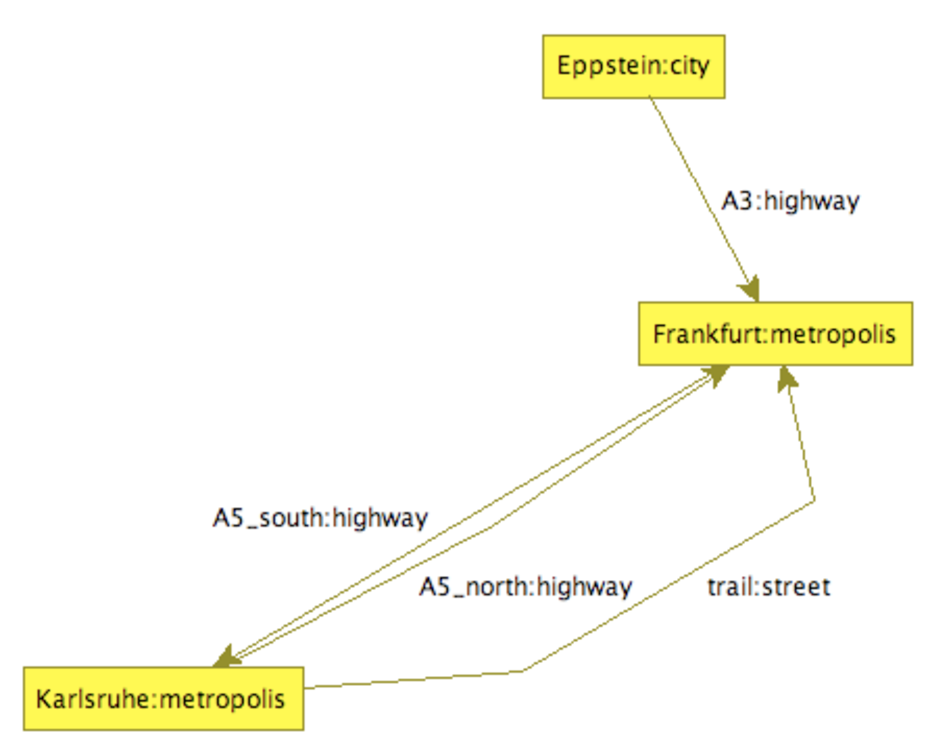
\includegraphics[width=8.5cm]{fig/map}}
\end{center}

This graph is valid but not strict valid.
\begin{grshell} 
> validate
The graph is valid.
> validate strict
The graph is NOT valid:
  CAE: city "Eppstein" -- highway "A3" --> metropolis "Frankfurt" not specified
  CAE: metropolis "Karlsruhe" -- street "trail" --> metropolis "Frankfurt" not specified
>
\end{grshell}
\end{example}

\begin{rail}
  'validate' ('exitonfailure')? 'xgrs' GRS
\end{rail}\ixkeyw{validate}\ixkeyw{grs}
Validates\indexmain{validate} if the current working graph satisfies the \indexed{graph rewrite sequence} given.
Before the graph rewrite sequence is executed, the instance graph gets cloned;
the sequence operates on the clone, allowing you to change the graph as you want to, without influence on the host graph.
Validation fails iff the xgrs fails.
This gives a rather costly but extremely flexible and powerful mechanism to specify graph constraints.
The GrShell is exited with an error code if \texttt{exitonfailure} is specified and the validation fails.


\subsection{Visited Flag Commands}

\begin{rail}
'Variable' '=' 'allocvisitflag'
\end{rail}\ixkeyw{allocvisitflag}\label{allocvisitflag}
Allocates space for a visited flag in the elements of the graph and returns the id of the visited flag (integer number), starting at 0.
Afterwards, the visited flag of the id can be read and written within the rules by the \texttt{visited}-expression and the \texttt{visited}-assignment,
as well as by the \texttt{isvisited} and \texttt{setvisited} shell commands.
The first visited flags are stored in some excess bytes of the graph elements and are thus essentially for free, but if this implementation defined space is used up completely, the information is stored in dictionaries.

\begin{rail}
'freevisitflag' 'Variable'
\end{rail}\ixkeyw{freevisitflag}
Frees the space previously allocated for the visited flag; afterwards you must not access it anymore. 
The value stored in the variable must be of integer type, stemming from a previous allocation.

\begin{rail} 
'setvisited' GraphElement 'flagId' 'BooleanValue'
\end{rail}\ixkeyw{setvisited}
Sets the visited status of the graph element of the flag id the given boolean value; visited flags are normally written by rules of the rule language.

\begin{rail}
'isvisited' GraphElement 'flagId'
\end{rail}\ixkeyw{isvisited}
Returns the visited status of the graph element of the flag id; visited flags are normally read by tests and rules of the rule language.


\subsection{Graph Input and Output Commands}
\label{outputcmds}

\begin{rail}
  'save' 'graph' Filename
\end{rail}\ixkeyw{save}\ixkeyw{graph}
Dumps\indexmain{dumping graph} the current graph as \GrShell\ script\indexmain{graph rewrite script} into \emph{Filename}.
The created script includes
\begin{itemize}
  \item selecting the backend
  \item creating a new graph with all nodes and edges (including their persistent names)
  \item restoring the variables
  \item restoring the visualisation styles
\end{itemize}
but not necessarily using the same commands you typed in during construction. 
Such a script can be loaded and executed by the \texttt{include} command (see Section~\ref{commcommands}).

\begin{rail}
  'export' Filename.grs (withvariables)?
\end{rail}\ixkeyw{export}
Exports an instance graph in GRS format, which is a reduced \GrShell\ script (it can get imported and exported on API level\ref{sub:imexport} without using the \GrShell\).
It contains the \texttt{new graph} command, followed by \texttt{new node} commands, followed by \texttt{new edge} commands.
If \texttt{withvariables} is specified, the variables are exported, too.
The export is only complete with the model of the graph given in the \texttt{.gm} file.
Exporting fails if the graph model contains attributes of \texttt{object}-type.
The \texttt{save} command is for saving a \GrShell\ session including visualization styles, the goal of the \texttt{export} command is graph rewrite system interoperability.

\begin{rail}
  'export' Filename.gxl
\end{rail}\ixkeyw{export}
Exports an instance graph and a graph model in GXL format \ref{}, which is somewhat of a standard format for graphs of graph rewrite systems, but suffers from the well-known XML problems -- it is barely human-readable and bloated.
Exporting fails if the graph model contains attributes of \texttt{set<S>}-,\texttt{map<S,T>}-, or \texttt{object}-type.

\begin{rail}
  'import' Filename.grs
\end{rail}\ixkeyw{import}
Imports the specified graph instance in GRS format (the \emph{reduced} \GrShell\ script, a saved graph can only be imported by \texttt{include} (but an exported graph can be imported by \texttt{include}, too)).
The referenced graph model must be available as \texttt{.gm}-file.

\begin{rail}
  'import' Filename.gxl (ModelOverride)?
\end{rail}\ixkeyw{import}
Imports the specified graph instance and model in GXL format.
If a model override of the form \texttt{Filename.gm} is specified, the given model will be used instead of the model in the GXL file.
The \texttt{.gxl}-graph must be compatible to the \texttt{.gm}-model.

\begin{note}
Normally you are not only interested in importing a GXL graph (and viewing it), but you want to execute actions on it.
The problem is that the actions are model dependent.
So, in order to apply actions, you must use a model override, which works this way:
\begin{enumerate}
\item \texttt{new graph "YourName.grg"}\\
This creates the model library lgsp-YourNameModel.dll
and the actions library lgsp-YourNameActions.dll
(which depends on the model library generated from the \texttt{"using YourName;"}).
\item \texttt{import InstanceGraphOnly.gxl YourName.gm}\\
This imports the instance graph from the .gxl but uses the model specified
in YourName.gm (it must fit to the model in the .gxl in order to work).
\item \texttt{select actions lgsp-YourNameActions.dll}\\
This loads the actions from the actions library in addition to the already
loaded model and instance graph (cf. \ref{grsthings}).
\item Now you are ready to use the actions.
\end{enumerate}
\end{note}


\subsection{Graph Manipulation Commands}
\label{mani}
Graph manipulation commands alter existing graphs; they allow to create and delete graph elements and change attributes. 
These are tasks which should be carried by the rules of the rule language -- the commands are mainly used as elementary instructions in graph input and output.

\begin{rail}
  'new' (() | Text) (() | ':' NodeType (() | Constructor))
\end{rail}\ixkeyw{new}
Creates a new node within the current graph.
Optionally a variable \emph{Text} is assigned to the new node.
If \emph{NodeType} is supplied, the new node will be of type \emph{NodeType} and attributes can be initialized by a constructor.
Otherwise the node will be of the base node class type \emph{Node}.
\begin{note}
The \GrShell\ can reassign \indexed{variable}s. 
This is in contrast to the rule language (chapter~\ref{chaprulelang}), where we use \emph{names}\indexmain{name}.
\end{note}

\begin{rail}
  'new' Node '-' (()|Text) \\ (() | ':' EdgeType (() | Constructor)) '->' Node
\end{rail}\ixkeyw{new}
Creates a new edge within the current graph between the specified nodes, directed towards the second \emph{Node}.
Optionally a variable \emph{Text} is assigned to the new edge.
If \emph{EdgeType} is supplied, the new edge will be of type \emph{EdgeType} and attributes can be initialized by a constructor.
Otherwise the edge will be of the base edge class type \emph{Edge}.

\begin{rail}
  Constructor : '(' (() | (dollar '=' Text (() | ',' Attributes) | Attributes)) ')';
  Attributes : AttributeName '=' (Text | Number) + ',' ;
\end{rail}\indexmain{\texttt{\$}}\ixnterm{Constructor}\ixnterm{Attributes}
A \indexed{constructor} is used to initialize a new graph element (see \texttt{new \dots} below).
A comma separated list of \indexed{attribute} declarations is supplied to the constructor.
Available attribute names are specified by the graph model of the current working graph.
All the undeclared attributes will be initialized with \indexed{default value}s, depending on their type (int $\leftarrow$ \texttt{0}, enum $\leftarrow$ unspecified; boolean $\leftarrow$ \texttt{false}; float, double $\leftarrow$ \texttt{0.0}; string $\leftarrow$ \texttt{""}).\\
The \texttt{\$} is a special attribute name: a unique identifier of the new graph element.
This identifier is also called \newterm{persistent name} (see Example~\ref{persistentex}).
This name can be specified by a constructor only.
TODO: set/map constructor

\begin{rail}
  'delete' 'node' Node
\end{rail}\ixkeyw{delete}\ixkeyw{node}
Deletes the node \emph{Node} from the current graph.
Incident edges will be deleted as well.

\begin{rail}
  'delete' 'edge' Edge
\end{rail}\ixkeyw{delete}\ixkeyw{edge}
Deletes the edge \emph{Edge} from the current graph.

\begin{rail}
  GraphElement '.' AttributeName '=' (Text | Number) ;
\end{rail}
Set the \indexed{attribute} \emph{AttributeName} of the graph element \emph{GraphElement} to the value of \emph{Text} or \emph{Number}.

  
\subsection{Graph and Model Query Commands}

todo: n.a, e.a shows the content of the attribute
todo: change this to show n.a, show e.a for consistency?

\begin{rail}
  'show' (() | 'num') ('nodes' (() | (() | 'only') NodeType) | 'edges' (() | (() | 'only') EdgeType))
\end{rail}\ixkeyw{show}\ixkeyw{num}\ixkeyw{nodes}\ixkeyw{edges}\ixkeyw{only}
Gets the \indexed{persistent name}s and the types of all the nodes/edges of the current graph. 
If a node type or edge type is supplied, only elements compatible to this type are considered. 
The \texttt{only} keyword excludes subtypes. Nodes/edges without persistent names are shown with a pseudo-name.
If the command is specified with \texttt{num}, only the number of nodes/edges will be displayed.

\begin{rail}
  'show' ('node' | 'edge') 'types'
\end{rail}\ixkeyw{show}\ixkeyw{node}\ixkeyw{edge}
Gets the node/edge types of the current graph model.

\begin{rail}
'show' ('node' ('super' | 'sub') 'types' NodeType | 'edge' ('super' | 'sub') 'types' EdgeType)
\end{rail}\ixkeyw{show}\ixkeyw{node}\ixkeyw{edge}\ixkeyw{super}\ixkeyw{sub}\indexmain{inheritance}
Gets the inherited/descendant types of \emph{NodeType}/\emph{EdgeType}.

\begin{rail}
  'show' ('node' 'attributes' (() | (() | 'only') NodeType) | 'edge' 'attributes' (() | (() | 'only') EdgeType))
\end{rail}\ixkeyw{show}\ixkeyw{node}\ixkeyw{edge}\ixkeyw{only}
Gets the available node/edge \indexed{attribute} types.
If \emph{NodeType}/\emph{EdgeType} is supplied, only attributes defined in \emph{NodeType}/\emph{EdgeType} are diplayed.
The \texttt{only} keyword excludes inherited attributes.\\
\begin{note}
The \texttt{show nodes/edges attributes\dots} command covers types and \emph{inherited} types.
This is in contrast to the other \texttt{show\dots} commands where types and \emph{sub}types are specified or the direction in the type hierarchy is specified explicitly, respectively.
\end{note}

\begin{rail}
 'show' ('node' Node | 'edge' Edge)
\end{rail}\ixkeyw{show}\ixkeyw{node}\ixkeyw{edge}
Gets the attribute types and values of a specific graph element.

\begin{rail}
 'show' 'var' Var
\end{rail}\ixkeyw{show}\ixkeyw{variable}
Displays the type and value of the specified variable.

\begin{rail}
  'show' GraphElement '.' AttributeName
\end{rail}\ixkeyw{show}\ixkeyw{attribute}
Displays the value of the specified attribute.

\begin{rail}
  'node' 'type' Node 'is' Node | 'edge' 'type' Edge 'is' Edge
\end{rail}\ixkeyw{node}\ixkeyw{edge}\ixkeyw{type}\ixkeyw{is}
Gets the information whether the first element is \indexed{type-compatible}\indexmainsee{compatible types}{type-compatible} to the second element.


\subsection{Graph Visualization Commands}

\begin{rail}
  'show' 'graph' ExecutableName (() | Text)
\end{rail}\ixkeyw{show}\ixkeyw{graph}
Dumps the current graph in \indexed{VCG} format into a temporary file.
The temporary VCG file will be passed to the program \emph{ExecutableName} as first parameter;
further parameters, such as program options, can be specified by \emph{Text}.
If you use \yComp\footnote{See Section~\ref{tools:ycomp}.}\indexmain{yComp} as executable (\texttt{show graph ycomp}), this may look like
\begin{center}
  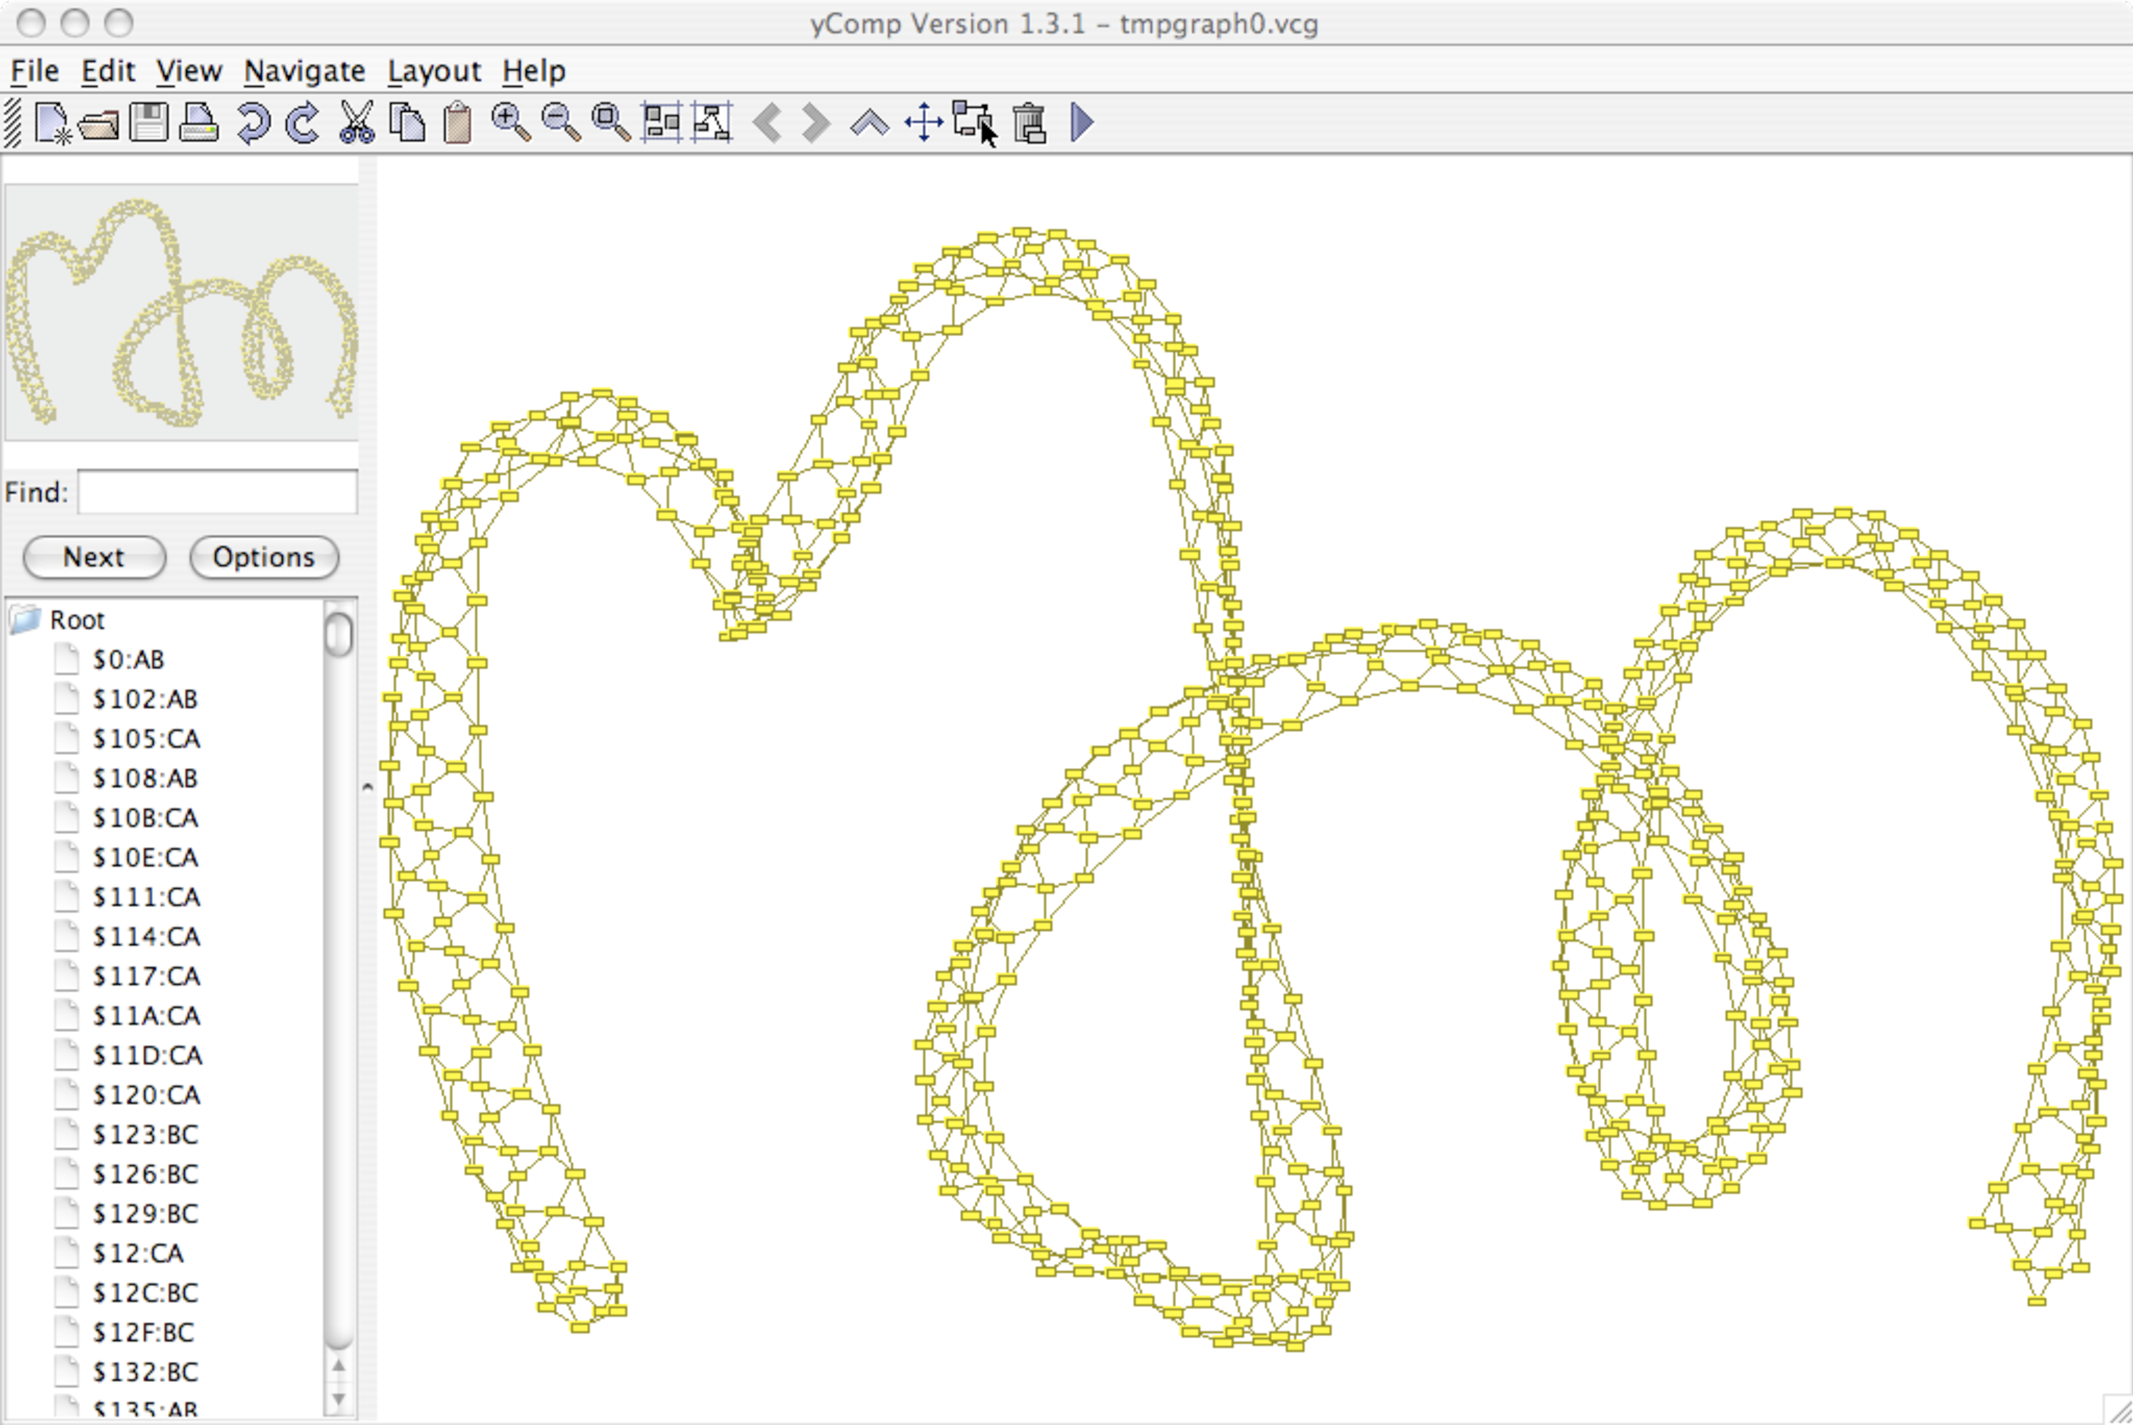
\includegraphics[width=0.75\linewidth]{fig/showgraph}
\end{center}  
The temporary file will be deleted, when the application \emph{Filename} is terminated if \GrShell\ is still running at this time.

\begin{rail}
  'dump' 'graph' Filename
\end{rail}\ixkeyw{dump}\ixkeyw{graph}
Dumps the current graph in \indexed{VCG} format into the file \emph{Filename}.\\

The following commands control the style of the VCG output. This affects \texttt{dump graph}, \texttt{show graph}, and \texttt{enable debug}. 
\begin{rail}
  'dump' 'set' 'node' (() | 'only') NodeType \\ (('color' | 'textcolor' | 'bordercolor') Color | 'shape' Text | 'labels' ('on' | 'off' | Text)) ;
\end{rail}\ixkeyw{dump}\ixkeyw{set}\ixkeyw{node}\ixkeyw{only}\ixkeyw{color}\ixkeyw{textcolor}\ixkeyw{bordercolor}\ixkeyw{shape}\ixkeyw{labels}
Sets the \indexed{color}, text color, border color, the shape or the label of the nodes of type \emph{NodeType} and all of its subtypes.
The keyword \texttt{only} excludes the subtypes. The available colors are specified at the begin of this chapter. 
The following shapes are supported: \texttt{box}, \texttt{triangle}, \texttt{circle}, \texttt{ellipse}, \texttt{rhom}, \texttt{hexagon}, \texttt{trapeze}, \texttt{uptrapeze}, \texttt{lparallelogram}, \texttt{rparallelogram}.
Those are shape names of \yComp\ (for a VCG definition see~\cite{vcg}).
The default labeling is set to \texttt{on} with \texttt{Name:Type}, it can be overwritten by an specified label string (e.g. the source code line originating the node in a program graph) or switched off.

\begin{rail}
  'dump' 'set' 'edge' (() | 'only') EdgeType \\ (('color' | 'textcolor') Color | 'labels' ('on' | 'off' | Text));
\end{rail}\ixkeyw{dump}\ixkeyw{set}\ixkeyw{edge}\ixkeyw{only}\ixkeyw{color}\ixkeyw{textcolor}\ixkeyw{labels}
Sets the color, text color or label of the edges of type \emph{EdgeType} and all of its subtypes.
The keyword \texttt{only} excludes the subtypes. The available colors are specified at the begin of this chapter.
The default labeling is set to \texttt{on} with \texttt{Name:Type}, it can be overwritten by an specified label string or switched off.

\begin{rail}
  'dump' 'add' 'node' ('only')? NodeType 'exclude' ;
\end{rail}\ixkeyw{dump}\ixkeyw{add}\ixkeyw{node}\ixkeyw{only}\ixkeyw{exclude}
Excludes nodes of type \emph{NodeType} and all of its subtypes as well as their incident edges from output.
The keyword \texttt{only} excludes the subtypes from exlusion, i.e.\ subtypes of \emph{NodeType} are dumped.

\begin{rail}
  'dump' 'add' 'node' ('only')? NodeType 'group' (GroupConstraints)? ;
GroupConstraints:
  'by' ('hidden')? GroupMode (IncAdjTypeConstraints)? ;
IncAdjTypeConstraints:
  ('only')? EdgeType ('with' ('only')? NodeType)? ;
\end{rail}\ixkeyw{dump}\ixkeyw{add}\ixkeyw{node}\ixkeyw{group}
Declares \emph{NodeType} and subtypes of \emph{NodeType} as \indexed{group node} type.
All the differently typed nodes that point to a node of type \emph{NodeType} 
(i.e.\ there is a directed edge between such nodes) will be grouped and visibly enclosed by the \emph{NodeType}-node.
\texttt{GroupMode} is one of \texttt{no},\texttt{incoming},\texttt{outgoing},\texttt{any}; \texttt{hidden} causes hiding of the edges by which grouping happens.
The \texttt{EdgeType} constrains the type of the edges which cause grouping, the \texttt{with} clause additionally constains the type of the adjacent node; 
\texttt{only} excludes subtypes.

The following example shows \emph{metropolis} ungrouped and grouped:
\begin{center}
  \fbox{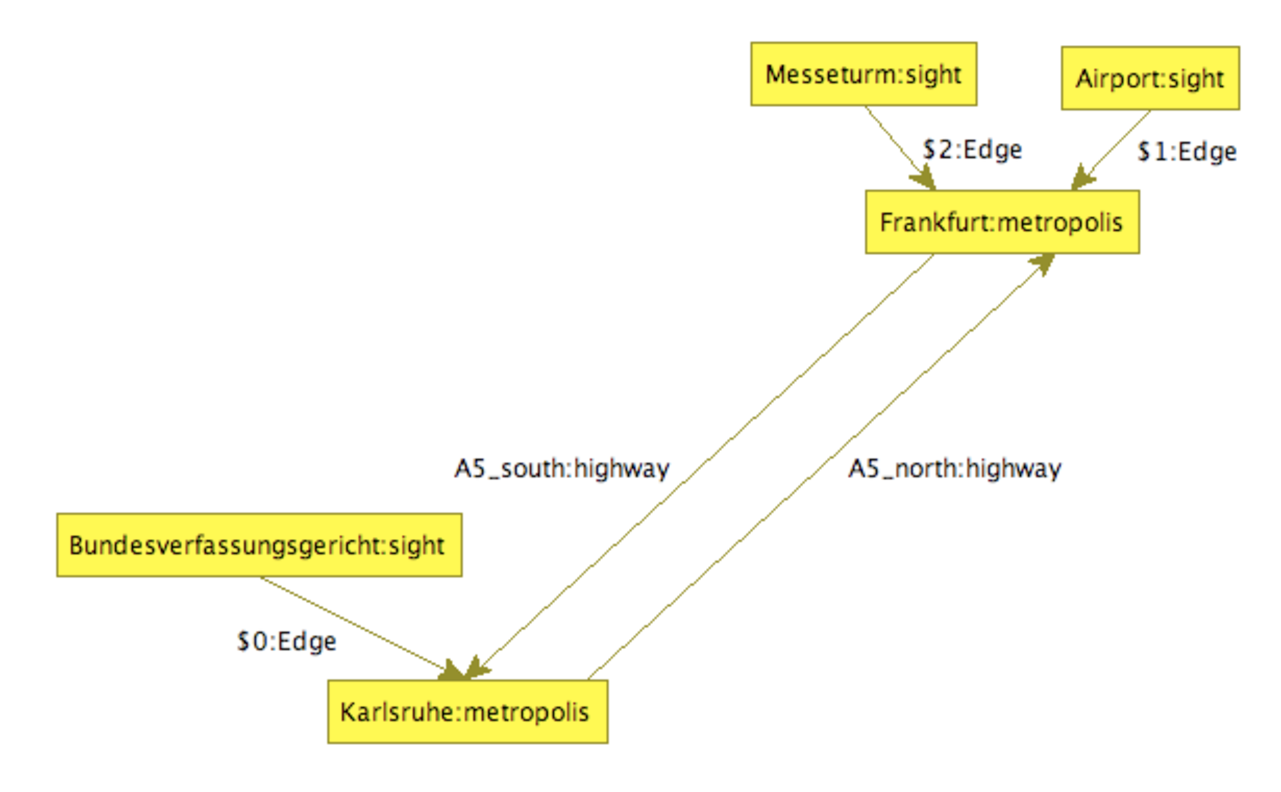
\includegraphics[width=0.45\linewidth]{fig/group2-1}}  \hfill \fbox{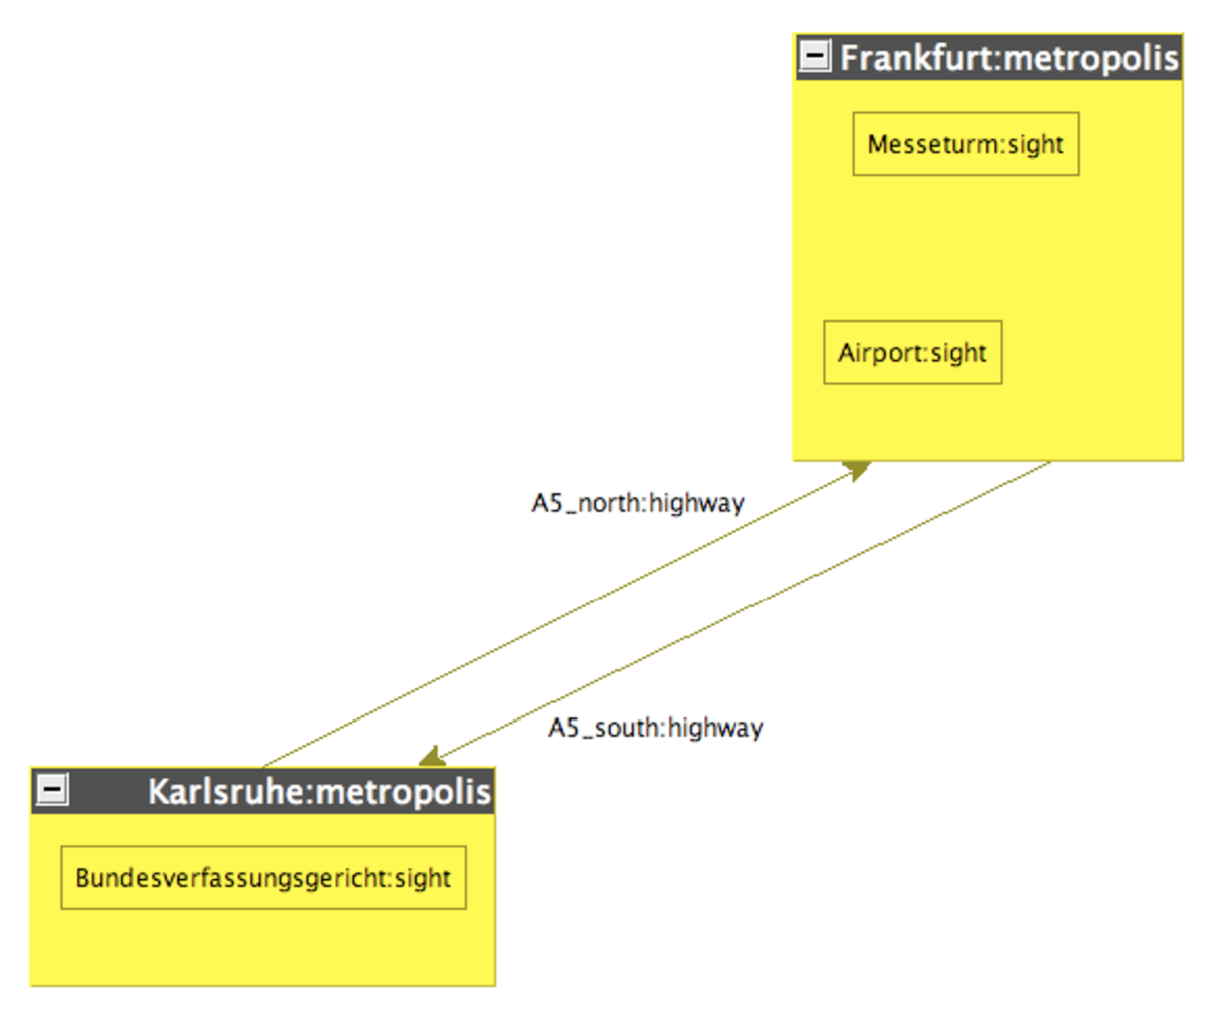
\includegraphics[width=0.45\linewidth]{fig/group2-2}}\\
  {\small right side: dumped with \texttt{dump add node metropolis group}}
\end{center}

\begin{rail}
  'dump' 'add' (() | 'only') ('node' NodeType | 'edge' EdgeType) \\ ('infotag' | 'shortinfotag') AttributeName
\end{rail}\ixkeyw{dump}\ixkeyw{add}\ixkeyw{only}\ixkeyw{node}\ixkeyw{edge}\ixkeyw{infotag}
Declares the \indexed{attribute} \emph{AttributeName} to be an ``\indexed{info tag}'' or ``\indexed{short info tag}''.
Info tags are displayed like additional node/edge \indexed{label}s, in format \texttt{Name=Value}, or \texttt{Value} only for short info tags. 
The keyword \texttt{only} excludes the subtypes of \emph{NodeType} resp.\ \emph{EdgeType}. 
In the following example \emph{river} and \emph{jam} are info tags:
\begin{center}
  \fbox{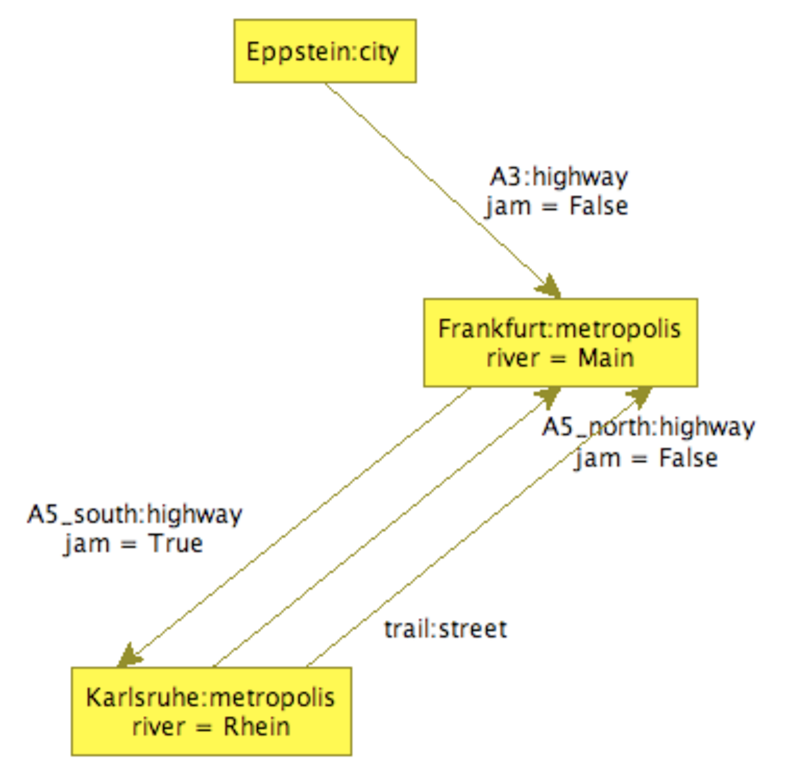
\includegraphics[width=0.5\linewidth]{fig/infotag}}
\end{center}

\begin{rail}
  'dump' 'reset'
\end{rail}\ixkeyw{dump}\ixkeyw{reset}
Resets all style options (\texttt{dump set}\dots) to their default values.


\begin{note}
Small graphs allow for fast visual understanding, but with an increasing number of nodes and edges they quickly loose this property.
The group commands are of outstanding importance to keep readability with increasing graph sizes
(e.g. for program graphs it allows to lump together expressions of a method inside the method node and attributes of the class inside the class node).
Additional helpers in keeping the graph readable are: 
the capability to exclude elements from dumping (the less hay in the stack the easier to find the needle),
the different colors and shapes to quickly find the elements of interest,
as well as the labels/infotags/shortinfotags to display the most important information directly. 
Choose the layout algorithm and the options delivering the best results for your needs, organic and compiler graph 
(an extension of hierarchic with automatic edge cutting -- marking cut edges by fat dots, showing the edge only on mouse over and allowing to jump to the other end on a mouse click)
should be tried first.
\end{note}


\subsection{Action Commands (XGRS)}\indexmain{action command}\indexmainsee{action}{graph rewrite sequence}
\label{grsthings}
An \emph{action} denotes a graph rewrite rule.

\begin{rail}
  'select' 'actions' Filename
\end{rail}\ixkeyw{select}\ixkeyw{actions}
Selects a \indexed{rule set}.
\emph{Filename} can either be a .NET assembly (e.g.\ ``rules.dll'') or a source file (``rules.cs'').
Only one rule set can be loaded simultaneously.

\begin{rail}
  'show' 'actions'
\end{rail}\ixkeyw{show}\ixkeyw{actions}
Lists all the rules of the loaded rule set, their parameters, and their return values.
Rules can return a set of graph elements.

\begin{rail}
  'custom' 'actions' (() | SpacedParameters)
\end{rail}\ixkeyw{custom}\ixkeyw{actions}
Executes an action specific to the current \indexed{backend}. 
If \emph{SpacedParameters} is omitted, a list of available commands will be displayed (for the LGSPBackend see Section~\ref{custom}).

\makeatletter
\begin{rail}
  GraphRewriteSequence: 'xgrs' SimpleRewriteSequence ;
\end{rail}\ixkeyw{grs}\indexmain{graph rewrite sequence}\indexmainsee{GRS}{graph rewrite sequence}\ixnterm{GraphRewriteSequence}
This executes the graph rewrite sequence \emph{SimpleRewriteSequence}.
See section \ref{sct:xgrs} for graph rewrite sequences.
Additionally to the variable assignment in rule-embedded graph rewrite sequences, you are also able to assign \emph{persistent names} to parameters via  \texttt{Variable = \@(Text)}.

Graph elements returned by rules can be assigned to variables\indexmain{variable} using \texttt{(Para\-meters) = \emph{Action}}\indexmain{parameter}. 
The desired variable identifiers have to be listed in \emph{Parameters}. 
Graph elements required by rules must be provided using \texttt{Action (Para\-meters)}, where \emph{Parameters} is a list of variable identifiers. 
For \indexed{undefined variables} see Section~\ref{ruledecls}, \emph{Parameters}.

% don't explain set/map commands, as they will be replaced by graph rewrite sequence terms
% they are given in the changelog, so if someone needs them now they are there
% but not fully officially documented, so that they can be dropped as soon as the sequences are extended


\section{Graphical Debugger}
\label{sct:debugger}
The \GrShell\ together with \yComp\ build \GrG's graphical debugger.

\subsection{Debugging Related Commands}

\begin{rail}
  'debug' ( 'enable' | 'disable' )
\end{rail}\ixkeyw{debug}\ixkeyw{enable}\ixkeyw{disable}
Enables and disables the \indexed{debug mode}.
The debug mode shows the current working graph in a \yComp\ window.
All changes to the working graph are tracked by \yComp\ immediately.  

\begin{rail}
  'debug' 'set' 'layout' ( (Text)? | 'option' Name String ) ;
\end{rail}\ixkeyw{debug}\ixkeyw{set}\ixkeyw{layout}
Sets the default graph \indexed{layout algorithm} to \emph{Text}.
If \emph{Text} is omitted, a list of available layout algorithms is displayed.
See Section~\ref{tools:ycomp} on \yComp\ layouters.
The \texttt{option} version allows to specify layout options by name value pairs.
The available layout options can be listed by the following command.

\begin{rail}
  'debug' 'get' 'layout' 'options';
\end{rail}\ixkeyw{debug}\ixkeyw{layout}
Prints a list of the available layout options of the layout algorithm.

\begin{rail}
  'debug' 'layout';
\end{rail}\ixkeyw{debug}\ixkeyw{layout}
Forces re-layout of the graph shown in yComp (same as pressing the play button within yComp).

\begin{rail}
  GraphRewriteSequence: 'debug' 'xgrs' SimpleRewriteSequence ;
\end{rail}\ixkeyw{debug}\ixkeyw{grs}\indexmain{graph rewrite sequence}\indexmainsee{GRS}{graph rewrite sequence}\ixnterm{GraphRewriteSequence}
This executes the graph rewrite sequence \emph{SimpleRewriteSequence} in the debugger\indexmain{debugger}.
Same as \texttt{xgrs SimpleRewriteSequence} in the previous section, but allows tracing the rewriting process step-by-step. 

\begin{rail}
'debug' 'apply' Rule
\end{rail}\ixkeyw{debug}\ixkeyw{apply}
The \texttt{debug apply} command allows to interactively select parameters for the execution of the rule \texttt{Rule}.
The parameters to select are specified by the wildcard elements \texttt{?}, they are given by double clicking at elements in the graph viewer yComp.

\begin{example}
\begin{grshelllet}
debug apply r(?, x, ?)
\end{grshelllet}
will prompt the user for input of the first and the third parameter, while the second one is taken from variable x.
\end{example}


\subsection{Using the Debugger}

During execution \yComp\footnote{Make sure, that the path to your \texttt{\indexed{yComp.jar}} package is set correctly in the \texttt{ycomp} shell script within \GrG's \texttt{/bin} directory.}
\indexmain{yComp} will display every single step. 
The debugger\indexmain{debugger} can be controlled by \GrShell. 
Remember that the \texttt{\%} modifier before a rule works as break point in a graph rewrite sequence.
The debug commands are shown in Table~\ref{tabdebug}. A run is shown in the following example \ref{ex:debug}.
\begin{table}[htbp]
  \begin{tabularx}{\linewidth}{|lX|} \hline
  \texttt{s}(tep) & Execute the next rewrite rule (match and rewrite)\\
  \texttt{d}(etailed step) & Execute a rewrite rule in a three-step procedure: matching, highlighting elements to be changed, doing rewriting \\
  \texttt{n}(ext) & Ascend one level up within the \indexed{Kantorowitsch tree} of the current rewrite sequence (see Example~\ref{ex:debug})\\
  (step) \texttt{o}(ut) & Continue execution until the end of the current loop. If the execution is not in a loop at this moment, the complete sequence will be executed\\
  (toggle) \texttt{b}(reakpoint) & Toggle a breakpoint at a rewrite rule, a true, or a false\\
  \texttt{r}(un) & Continue execution\\
  \texttt{a}(bort) & Cancel the execution immediately\\ \hline 
  \end{tabularx}
  \caption{\GrShell\ debug commands}
  \label{tabdebug}
\end{table}
%\begin{figure}[htbp]
%  \centering
%  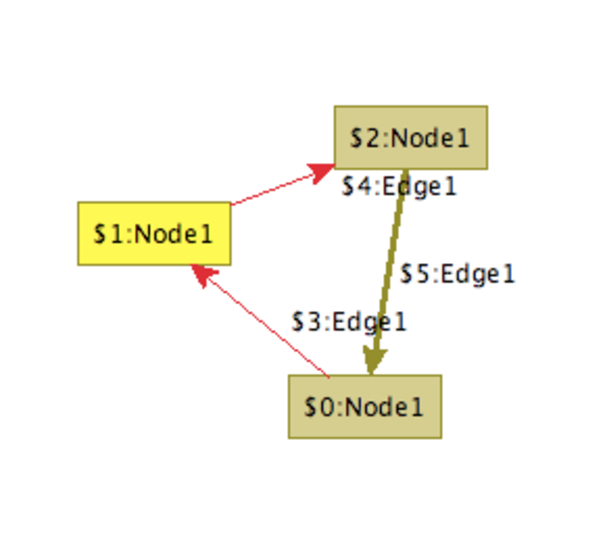
\includegraphics[width=0.25\linewidth]{fig/debug1}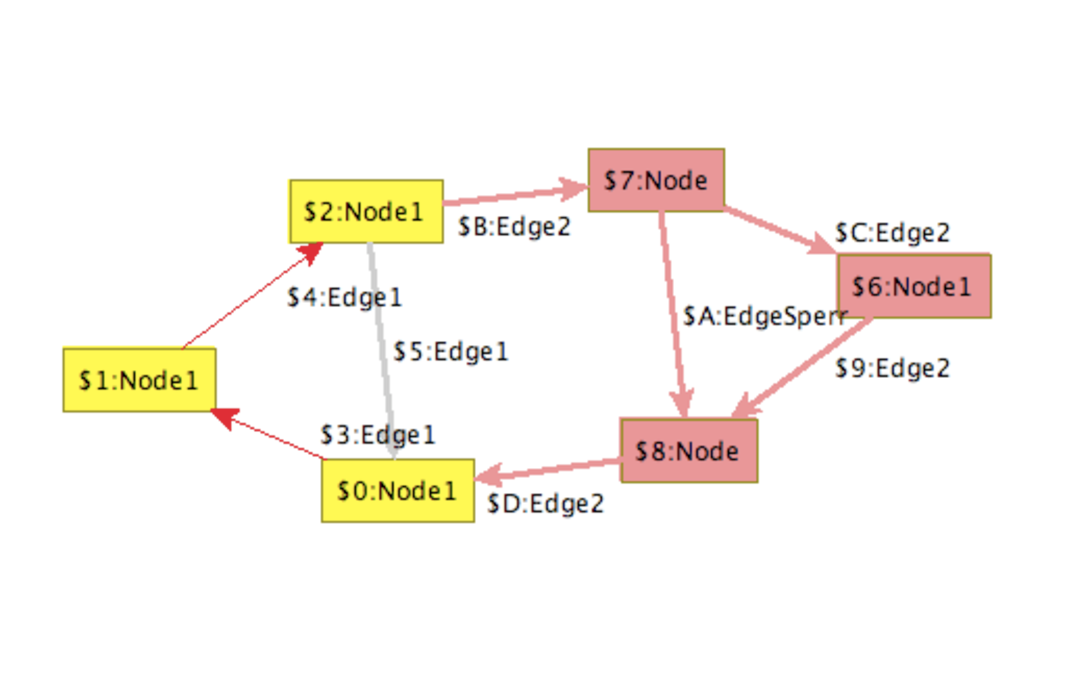
\includegraphics[width=0.4\linewidth]{fig/debug2}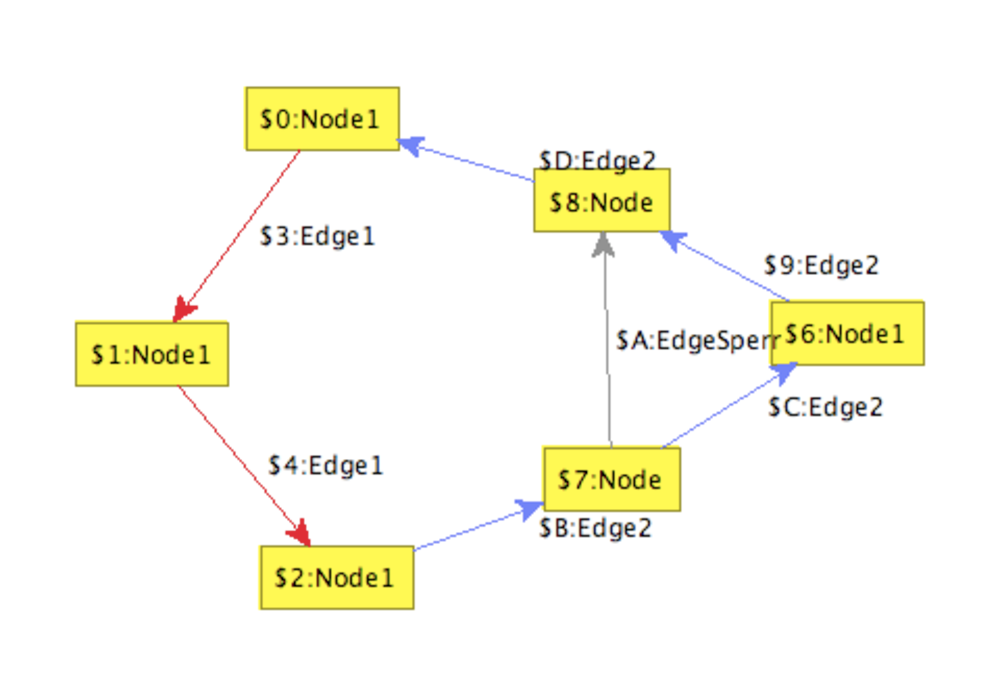
\includegraphics[width=0.4\linewidth]{fig/debug3}
%  \caption{Delayed step rule application.}
%  \label{figdebug}
%\end{figure}

\begin{figure}[htbp]
\begin{example}\label{ex:debug}  
We demonstrate the debug commands with a slightly adjusted script for the Koch snowflake from \GrG's examples (see also Section~\ref{fractals}). The graph rewriting sequence is
\begin{grshell}
debug xgrs (makeFlake1* & (beautify & doNothing)* & makeFlake2* & beautify*)[1]
\end{grshell}
\yComp\ will be opened with an initial graph (resulting from \texttt{grs init}):
\begin{center}
  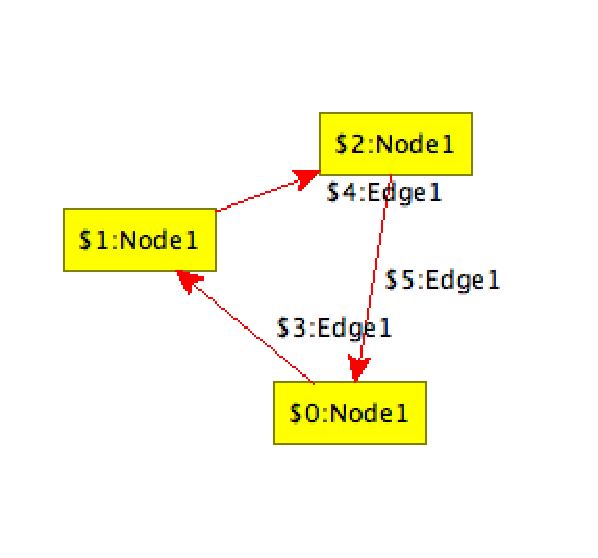
\includegraphics[width=0.3\linewidth]{fig/debug0tra}
\end{center}
We type \texttt{d}(etailed step) to apply \texttt{makeFlake1} step by step resulting in the following graphs:
\begin{center}
  \parbox{0.2\linewidth}{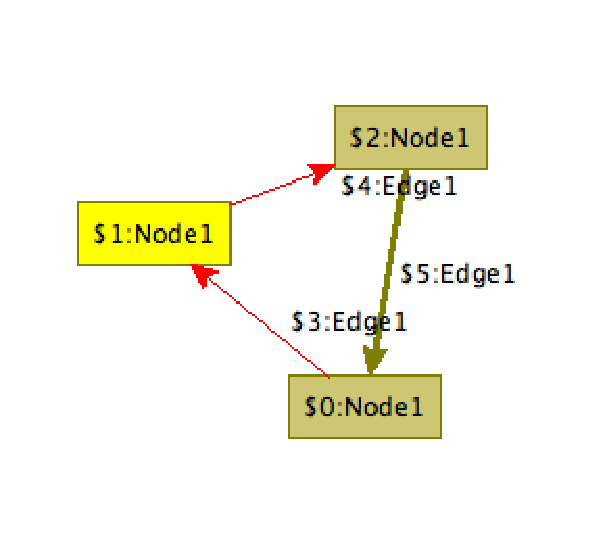
\includegraphics[width=\linewidth]{fig/debug1tra}}\parbox{0.375\linewidth}{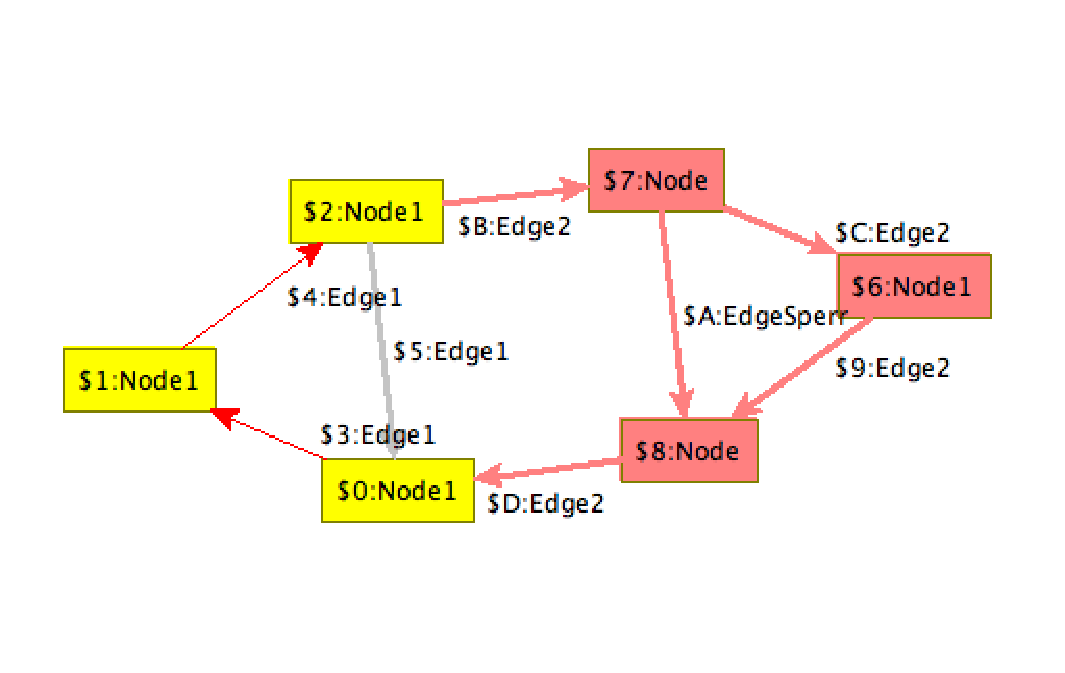
\includegraphics[width=\linewidth]{fig/debug2tra}}\parbox{0.375\linewidth}{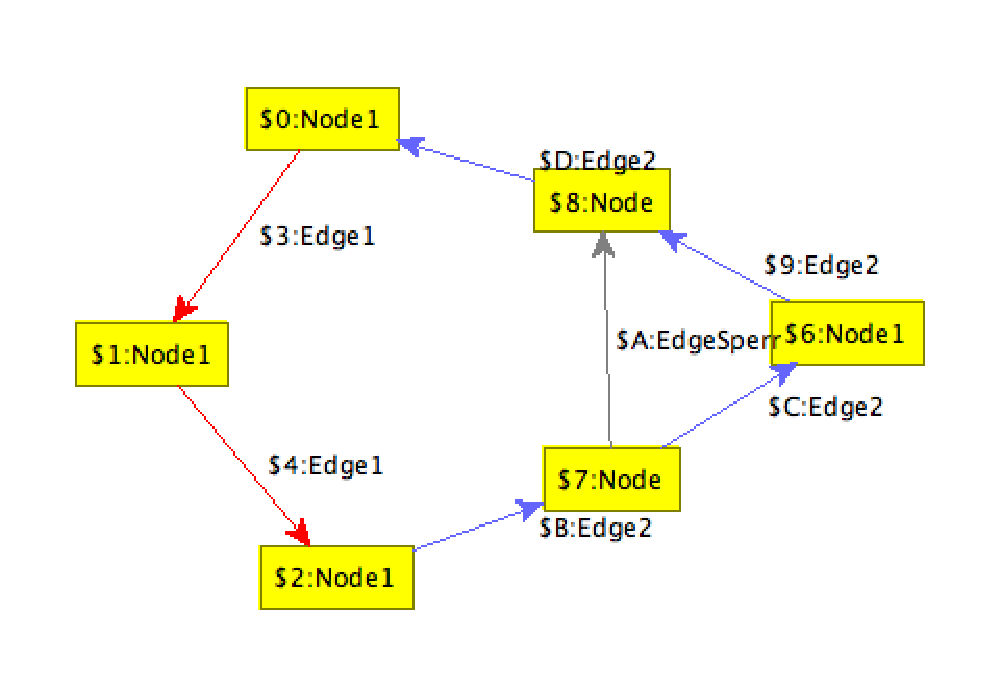
\includegraphics[width=\linewidth]{fig/debug3tra}}
\end{center}
The following table shows the ``break points'' of further debug commands, entered one after another:
\begin{center}
  \begin{tabular}{|l|l|} \hline
    \textbf{Command} & \textbf{Active rule} \\ \hline
    \texttt{s} & \texttt{makeFlake1} \\
    \texttt{o} & \texttt{beautify} \\
    \texttt{s} & \texttt{doNothing} \\
    \texttt{s} & \texttt{beautify} \\ 
    \texttt{n} & \texttt{beautify} \\ 
    \texttt{o} & \texttt{makeFlake2} \\
    \texttt{r} & --- \\ \hline
  \end{tabular}
\end{center}
\end{example}   
\end{figure}


\section{Backend Commands}
\label{backend}

\GrG\ is built to support multiple backends implementing the model and action interfaces of libGr.
This is roughly comparable to the different storage engines MySQL offers.
Currently only one backend is available, the libGr search plan backend, or short LGSPBackend.

\subsection{Backend selection and custom commands}

\begin{rail}
  'select' 'backend' Filename ( ( ) | ':' Parameters )
\end{rail}\ixkeyw{select}\ixkeyw{backend}
Selects a \indexed{backend} that handles graph and rule representation.
\emph{Filename} has to be a .NET assembly (e.g.\ \texttt{lgspBackend.dll}\indexmain{LGSPBackend}).
Comma-separated \indexed{parameter}s can be supplied optionally; if so, the backend must support these parameters.
By default the LGSPBackend is used.

\begin{rail}
  'show' 'backend'
\end{rail}\nopagebreak\ixkeyw{show}\ixkeyw{backend}
List all the parameters supported by the currently selected backend.
The parameters can be provided to the \texttt{select backend} command.

\begin{rail}
  'custom' 'graph' ( ( ) | SpacedParameters )
\end{rail}\ixkeyw{custom}\ixkeyw{graph}
Executes a command specific to the current backend.
If \emph{SpacedParameters} is omitted, a list of available commands will be displayed (for the LGSP backend see Sections~\ref{custom}).


\subsection{LGSPBackend Custom Commands}
\label{custom}

The \indexed{LGSPBackend} supports the following custom commands:

\begin{rail}
  'custom' 'graph' analyzegraph
\end{rail}\ixkeyw{custom}\ixkeyw{graph}
Analyzes\indexmain{analyzing graph} the current working graph.
The analysis data provides vital information for efficient \indexed{search plan}s.
Analysis data is available as long as \GrShell\ is running, i.e.\ when the working graph changes, the analysis data is still available but maybe obsolete.

\begin{rail}
  'custom' 'actions' gensearchplan (Action+)
\end{rail}\ixkeyw{custom}\ixkeyw{actions}
Creates a search plan for each rewrite rule \emph{Action} using a heuristic method and the analyzes data (if the graph has been analyzed by \texttt{custom graph analyze\_graph}).
Otherwise a \indexed{default search plan} is used.
For efficiency reasons it is recommended to do analyzing and search plan creation during the rewriting procedure.
Therefore the host graph should be in a stage ``similar'' to the final result.
Indeed there might be some trial-and-error steps necessary to get an efficient search plan.
A search plan is available as long as the current rule set remains loaded. 
Specify multiple rewrite rules instead of using multiple commands for each rule to improve the search plan generation performance.

\begin{rail}
  'custom' 'actions' setmaxmatches Number
\end{rail}\ixkeyw{custom}\ixkeyw{actions}
Sets the maximum amount of possible pattern matches to \emph{Number}.
This command affects the expression \texttt{[\emph{Rule}]}.
If \emph{Number} is less or equal to zero, the constraint is reset.



\chapter{Examples}
\label{anexample}

%%%%%%%%%%%%%%%%%%%%%%%%%%%%%%%%%%%%%%%%%%%%%%%%%%%%%%%%%%%%%%%%%%%%%%%%%%%%%%%%%%%%%%%%%%%%%%%%
\section{Fractals}\indexmain{example}
\label{fractals}
The \GrG\ package ships with samples for fractal generation. We will construct the \indexed{Sierpinski triangle} and the \indexed{Koch snowflake}. They are created by consecutive rule applications starting with the initial host graphs
\begin{center}
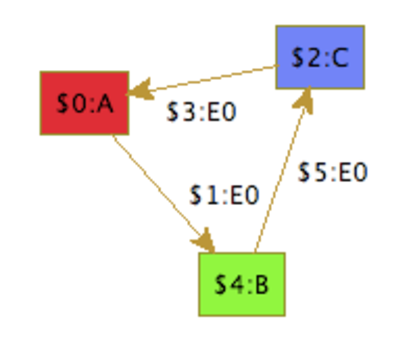
\includegraphics[width=4cm]{fig/startsir}\quad\quad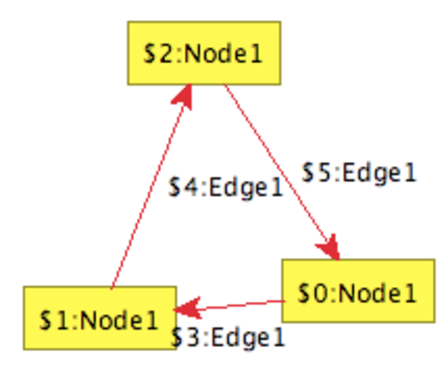
\includegraphics[width=4cm]{fig/startkoch}
\end{center}
for the Sierpinski triangle resp.\ the Koch snowflake.
First of all we have to compile the model and rule set files. So execute in \GrG's \texttt{bin} directory
\begin{verbatim}
GrGen.exe ..\specs\sierpinski.grg
GrGen.exe ..\specs\snowflake.grg
\end{verbatim}
or
\begin{verbatim}
mono GrGen.exe ../specs/sierpinski.grg
mono GrGen.exe ../specs/snowflake.grg
\end{verbatim}
respectively. If you are on a Unix-like system you have to adjust the path separators of the \GrShell\ scripts. Just edit the first three lines of \texttt{/test/Sierpinski.grs} and \texttt{/test/Snowflake.grs}. And as we have the file \texttt{Sierpinski.grs} already opened, we can increase the number of iterations to get even more beautiful graphs\footnote{Be careful: The running time increases exponentially in the number of iterations.}. Just follow the comments. Be careful when increasing the number of iterations of Koch's snowflake---\yComp's \indexed{layout algorithm} might need some time and attempts to layout it nicely.
We execute the Sierpinski script by
\begin{verbatim}
GrShell.exe ..\test\Sierpinski.grs
\end{verbatim}
or
\begin{verbatim}
mono GrShell.exe ../test/Sierpinski.grs
\end{verbatim}
respectively. Because both of the scripts are using the debug mode, we complete execution by typing \texttt{r}(un). See Section~\ref{grsthings} for further information. The resulting graphs should look like Figures~\ref{figsierp} and~\ref{figsnowflake}.
\begin{figure}[htbp]
  \centering
  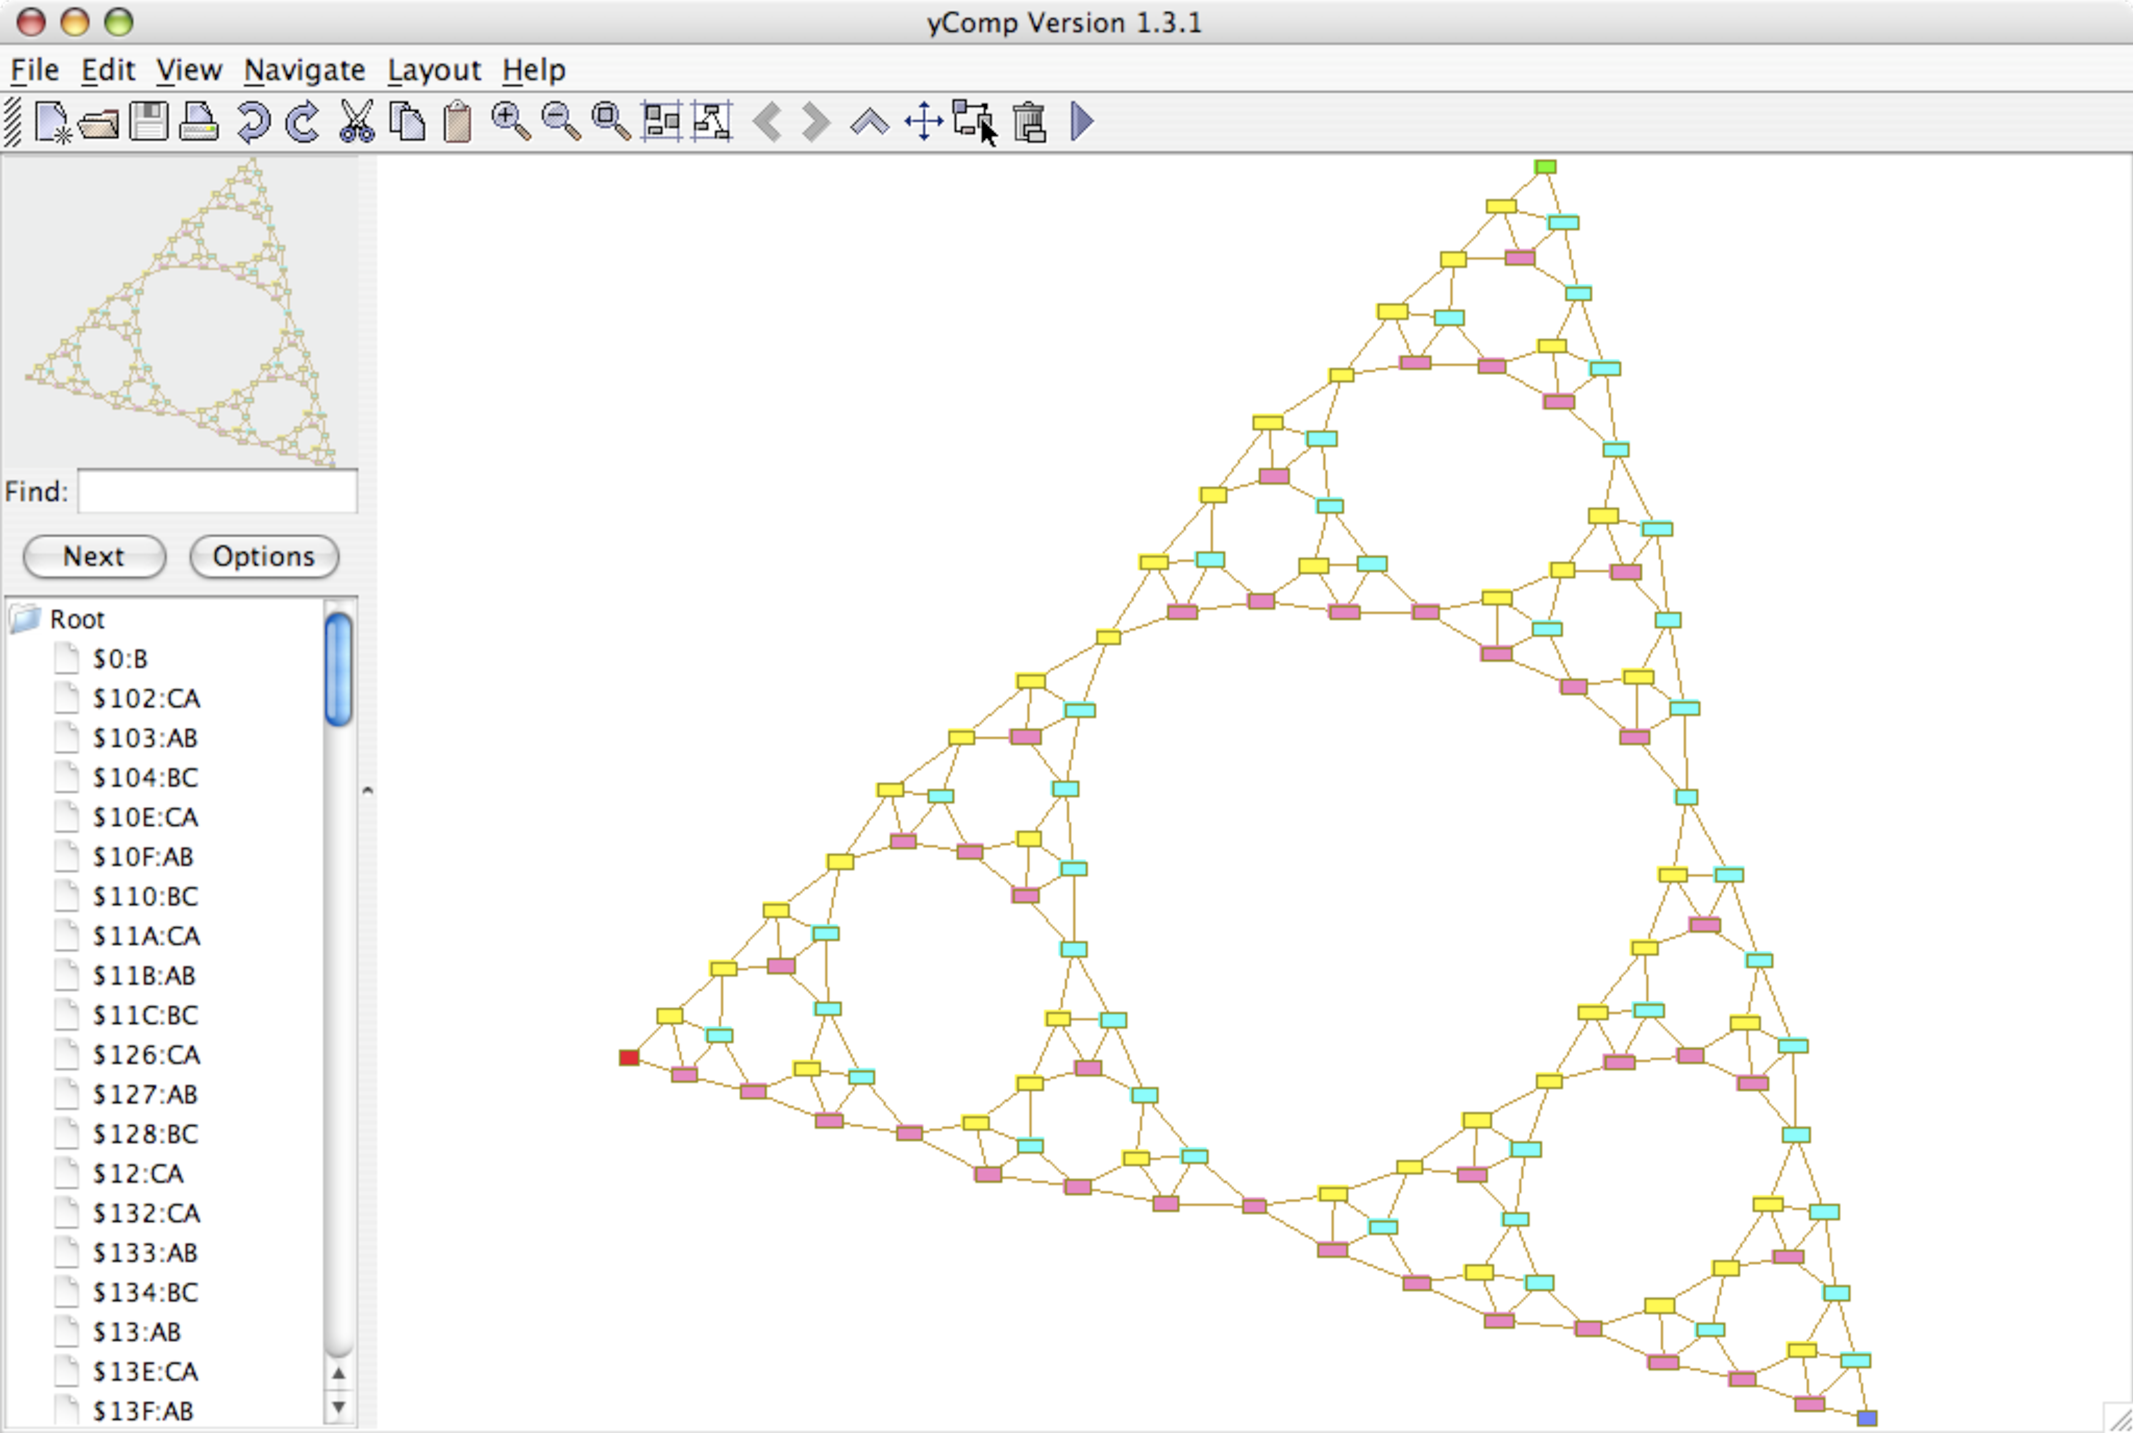
\includegraphics[width=\textwidth]{fig/sierpinski}
  \caption{Sierpinski triangle}
  \label{figsierp}
\end{figure}
\begin{figure}[htbp]
  \centering
  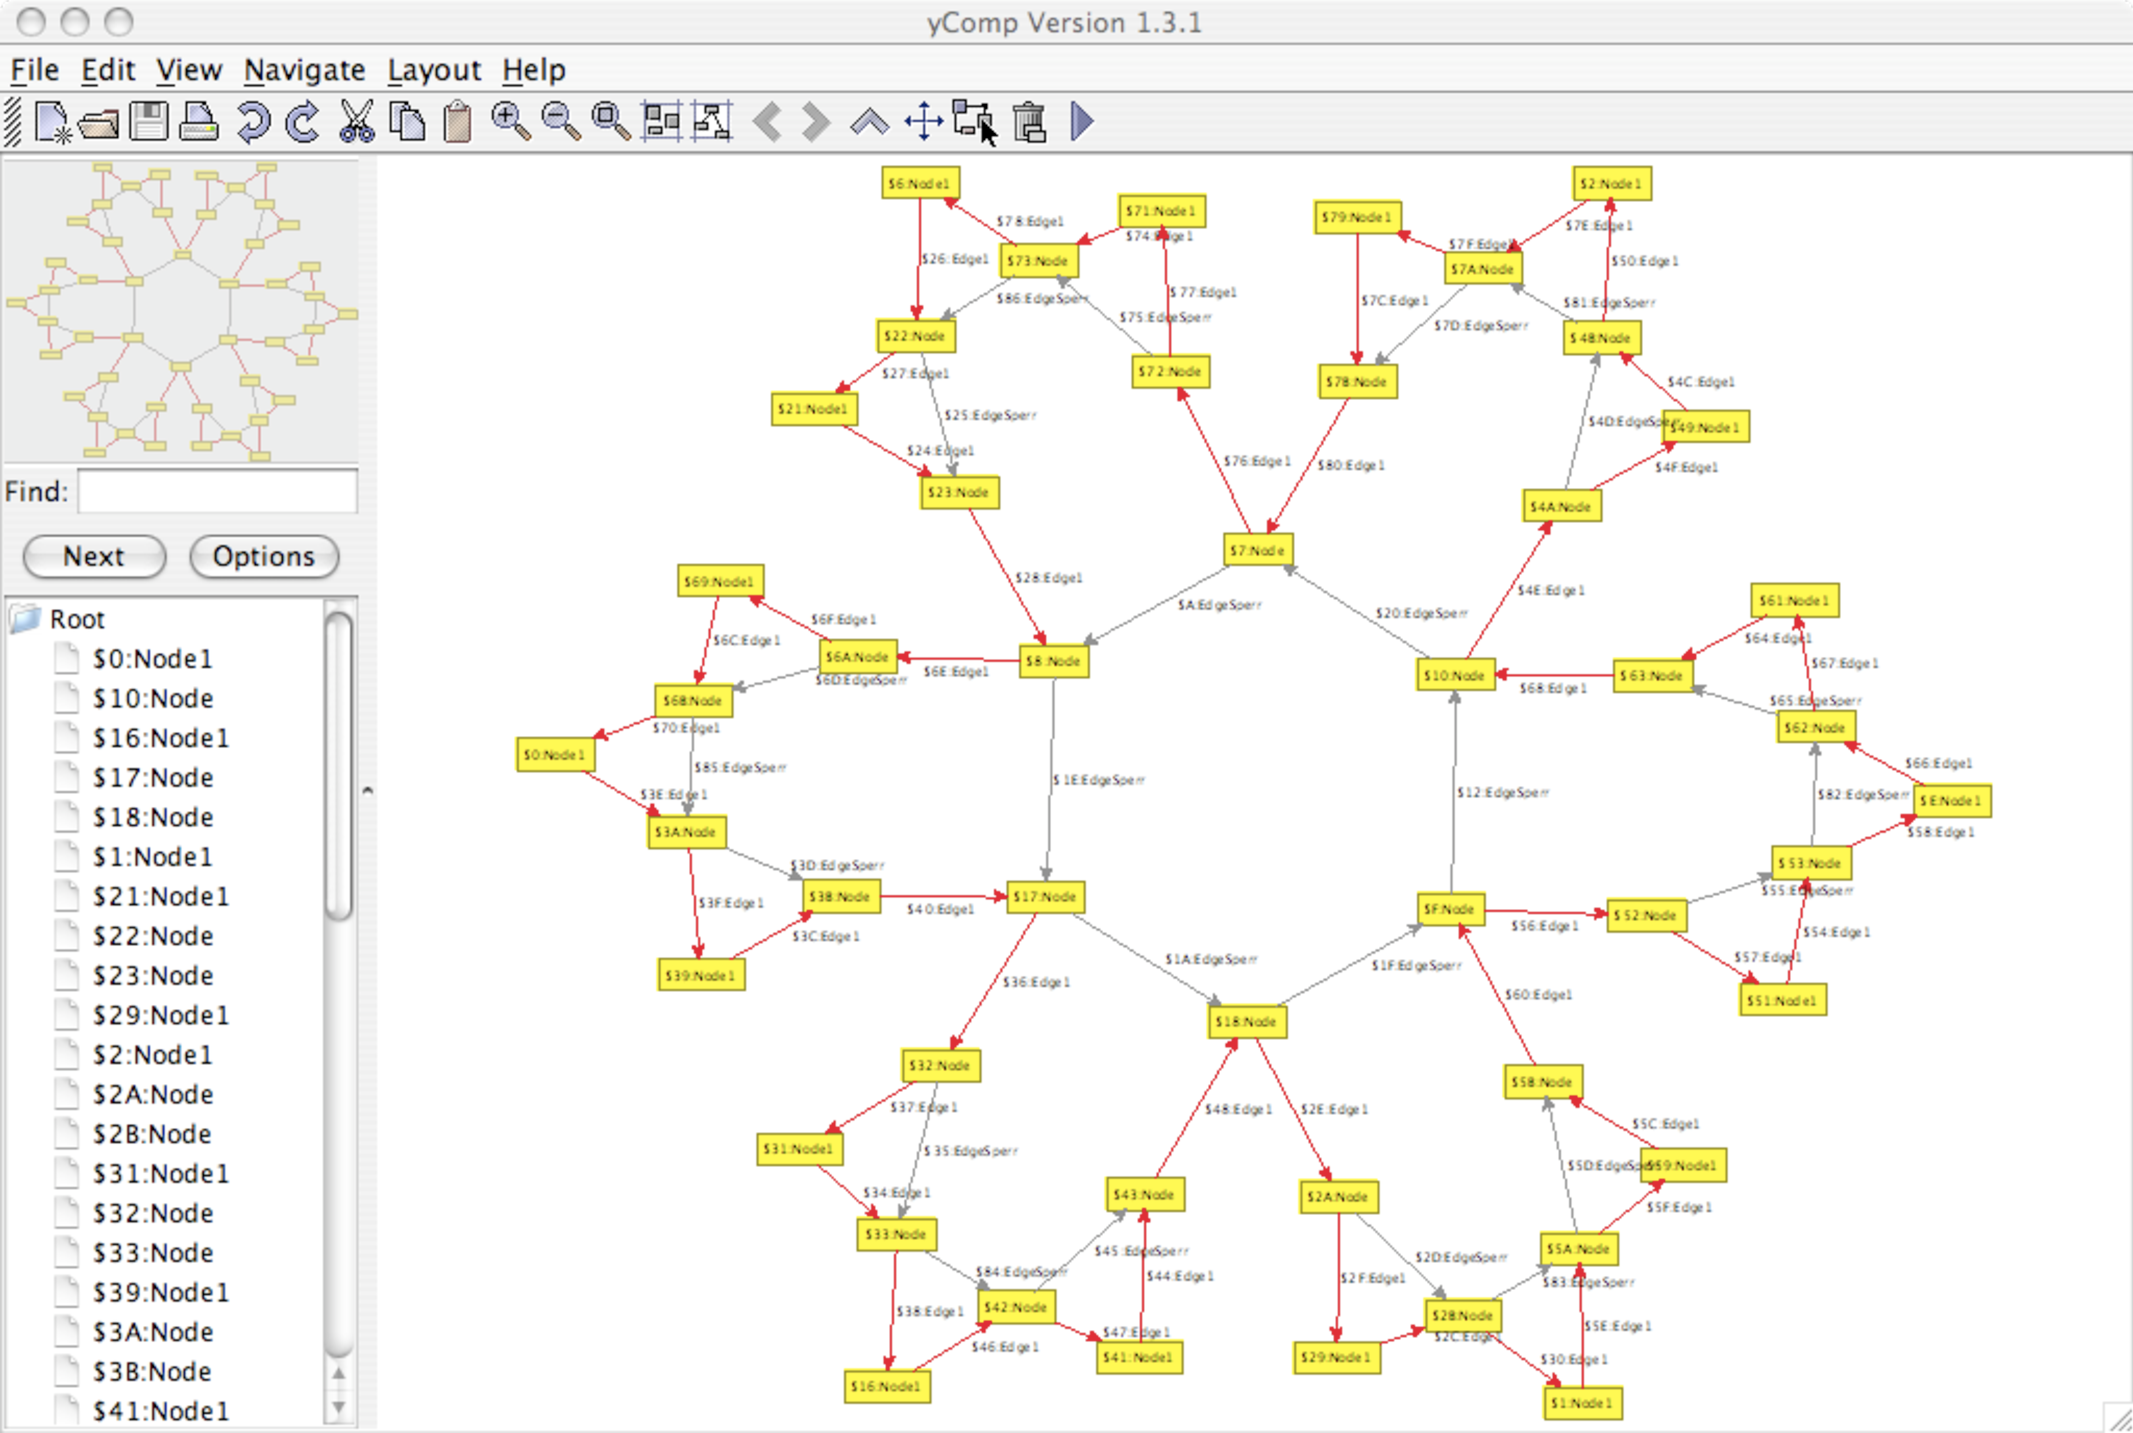
\includegraphics[width=\textwidth]{fig/snowflake}
  \caption{Koch snowflake}
  \label{figsnowflake}
\end{figure}
\vfill\pagebreak


%%%%%%%%%%%%%%%%%%%%%%%%%%%%%%%%%%%%%%%%%%%%%%%%%%%%%%%%%%%%%%%%%%%%%%%%%%%%%%%%%%%%%%%%%%%%%%%%
\section{Busy Beaver}\indexmain{example}
We want \GrG\ to work as hard as a \indexed{busy beaver}~\cite{Kro:07,Dew:84}. Our busy beaver is a Turing machine that has got five states plus a ``halt''-state; it writes 1,471 bars onto the tape and terminates~\cite{MB:00}. So first of all we design a Turing machine as graph model. Besides, this example shows that \GrG\ is \indexed{Turing complete}.

We use the graph model and the rewrite rules to define a general Turing machine. Our approach is to basically draw the machine as a graph. The busy beaver logic is implemented by rule applications in \GrShell.

%-----------------------------------------------------------------------------------------------
\subsection{Graph Model}
The tape will be a chain of \texttt{TapePosition} nodes connected by right edges. A cell value is modeled by a reflexive \texttt{value} edge, attached to a \texttt{TapePosition} node. The leftmost and the rightmost cells (\texttt{TapePosition}) do not have an incoming and outgoing edge respectively. Therefore we have the node constraint $[0:1]$.
\begin{grgen}[firstnumber=last]
node class TapePosition;
edge class right
  connect TapePosition[0:1] --> TapePosition[0:1];

edge class value
  connect TapePosition[1] --> TapePosition[1];
edge class zero  extends value;
edge class one   extends value;
edge class empty extends value;

\end{grgen}
Furthermore we need states and transitions.
The machine's current configuration is modeled with a \texttt{RWHead} edge pointing to a \texttt{TapePosition} node.
\texttt{State} nodes are connected with \texttt{WriteValue} nodes via \texttt{value} edges, a \texttt{moveLeft}/\texttt{moveRight}/\texttt{dontMove} edge leads from a \texttt{WriteValue} node to the next state (cf.~the picture on page \pageref{fig:bbstart}).
\begin{grgen}[firstnumber=last]
node class State;

edge class RWHead;

node class WriteValue;
node class WriteZero extends WriteValue;
node class WriteOne extends WriteValue;
node class WriteEmpty extends WriteValue;

edge class moveLeft;
edge class moveRight;
edge class dontMove;
\end{grgen}

%-----------------------------------------------------------------------------------------------
\subsection{Rule Set}
Now the rule set: We begin the rule set file \texttt{Turing.grg} with
\begin{grgen}[firstnumber=1]
using TuringModel;

\end{grgen}
We need rewrite rules for the following steps of the Turing machine:
\begin{enumerate}
  \item Read the value of the current tape cell and select an outgoing edge of the current state.
  \item Write a new value into the current cell, according to the sub type of the \texttt{WriteValue} node.
  \item Move the read-write-head along the tape and select a new state as current state.
\end{enumerate}
As you can see a transition of the Turing machine is split into two graph rewrite steps: Writing the new value onto the tape and performing the state transition. We need eleven rules: Three rules for each step (for ``zero'', ``one'', and ``empty'') and two rules for extending the tape to the left and the right, respectively.
\begin{grgen}[firstnumber=last]
rule readZeroRule {
	s:State -h:RWHead-> tp:TapePosition -:zero-> tp;
	s -:zero-> wv:WriteValue;
	modify {
		delete(h);
		wv -:RWHead-> tp;
	}
}

\end{grgen}
We take the current state \texttt{s} and the current cell \texttt{tp} which is implicitly given by the unique \texttt{RWHead} edge and check whether the cell value is zero. Furthermore we check if the state has a transition for zero. The replacement part deletes the \texttt{RWHead} edge between \texttt{s} and \texttt{tp} and adds it between \texttt{wv} and \texttt{tp}. The remaining rules are analogous:
\begin{grgen}[firstnumber=last]
rule readOneRule {
	s:State -h:RWHead-> tp:TapePosition -:one-> tp;
	s -:one-> wv:WriteValue;
	modify {
		delete(h);
		wv -:RWHead-> tp;
	}
}

rule readEmptyRule {
	s:State -h:RWHead-> tp:TapePosition -:empty-> tp;
	s -:empty-> wv:WriteValue;
	modify {
		delete(h);
		wv -:RWHead-> tp;
	}
}

rule writeZeroRule {
	wv:WriteZero -rw:RWHead-> tp:TapePosition -:value-> tp;
	replace {
		wv -rw-> tp -:zero-> tp;
	}
}

rule writeOneRule {
	wv:WriteOne -rw:RWHead-> tp:TapePosition -:value-> tp;
	replace {
		wv -rw-> tp -:one-> tp;
	}
}

rule writeEmptyRule {
	wv:WriteEmpty -rw:RWHead-> tp:TapePosition -:value-> tp;
	replace {
		wv -rw-> tp -:empty-> tp;
	}
}

rule moveLeftRule {
	wv:WriteValue -:moveLeft-> s:State;
	wv -h:RWHead-> tp:TapePosition <-r:right- ltp:TapePosition;
	modify {
		delete(h);
		s -:RWHead-> ltp;
	}
}

rule moveRightRule {
	wv:WriteValue -:moveRight-> s:State;
	wv -h:RWHead-> tp:TapePosition -r:right-> rtp:TapePosition;
	modify {
		delete(h);
		s -:RWHead-> rtp;
	}
}

rule dontMoveRule {
	wv:WriteValue -:dontMove-> s:State;
	wv -h:RWHead-> tp:TapePosition;
	modify {
		delete(h);
		s -:RWHead-> tp;
	}
}

rule ensureMoveLeftValidRule {
	wv:WriteValue -:moveLeft-> :State;
	wv -:RWHead-> tp:TapePosition;
	negative {
		tp <-:right-;
	}
	modify {
		tp <-:right- ltp:TapePosition -:empty-> ltp;
	}
}

rule ensureMoveRightValidRule {
	wv:WriteValue -:moveRight-> :State;
	wv -:RWHead-> tp:TapePosition;
	negative {
		tp -:right->;
	}
	modify {
		tp -:right-> rtp:TapePosition -:empty-> rtp;
	}
}
\end{grgen}
Have a look at the negative conditions within the \texttt{ensureMove\dots} rules. They ensure that the current cell is indeed at the end of the tape: An edge to a right/left neighboring cell must not exist. Now don't forget to compile your model and the rule set with \texttt{GrGen.exe} (see Section~\ref{fractals}).

%-----------------------------------------------------------------------------------------------
\subsection{Rule Execution with \GrShell}

Finally we construct the busy beaver and let it work with \GrShell. The following script starts with building the Turing machine that is modeling the six states with their transitions in our Turing machine model:
\begin{grshell}[firstnumber=1]
select backend "../bin/lgspBackend.dll"
new graph "../lib/lgsp-TuringModel.dll" "Busy Beaver"
select actions "../lib/lgsp-TuringActions.dll"

# Initialize tape
new tp:TapePosition($="Startposition")
new tp -:empty-> tp

# States
new sA:State($="A")
new sB:State($="B")
new sC:State($="C")
new sD:State($="D")
new sE:State($="E")
new sH:State($ = "Halt")

new sA -:RWHead-> tp

# Transitions: three lines per state and input symbol for
#   - updating cell value
#   - moving read-write-head
# respectively

new sA_0: WriteOne
new sA -:empty-> sA_0
new sA_0 -:moveLeft-> sB

new sA_1: WriteOne
new sA -:one-> sA_1
new sA_1 -:moveLeft-> sD

new sB_0: WriteOne
new sB -:empty-> sB_0
new sB_0 -:moveRight-> sC

new sB_1: WriteEmpty
new sB -:one-> sB_1
new sB_1 -:moveRight-> sE

new sC_0: WriteEmpty
new sC -:empty-> sC_0
new sC_0 -:moveLeft-> sA

new sC_1: WriteEmpty
new sC -:one-> sC_1
new sC_1 -:moveRight-> sB

new sD_0: WriteOne
new sD -:empty-> sD_0
new sD_0 -:moveLeft->sE

new sD_1: WriteOne
new sD -:one-> sD_1
new sD_1 -:moveLeft-> sH

new sE_0: WriteOne
new sE -:empty-> sE_0
new sE_0 -:moveRight-> sC

new sE_1: WriteOne
new sE -:one-> sE_1
new sE_1 -:moveLeft-> sC

\end{grshell}
\quad\\Our busy beaver looks like this:\label{fig:bbstart}
\begin{center}
  \fbox{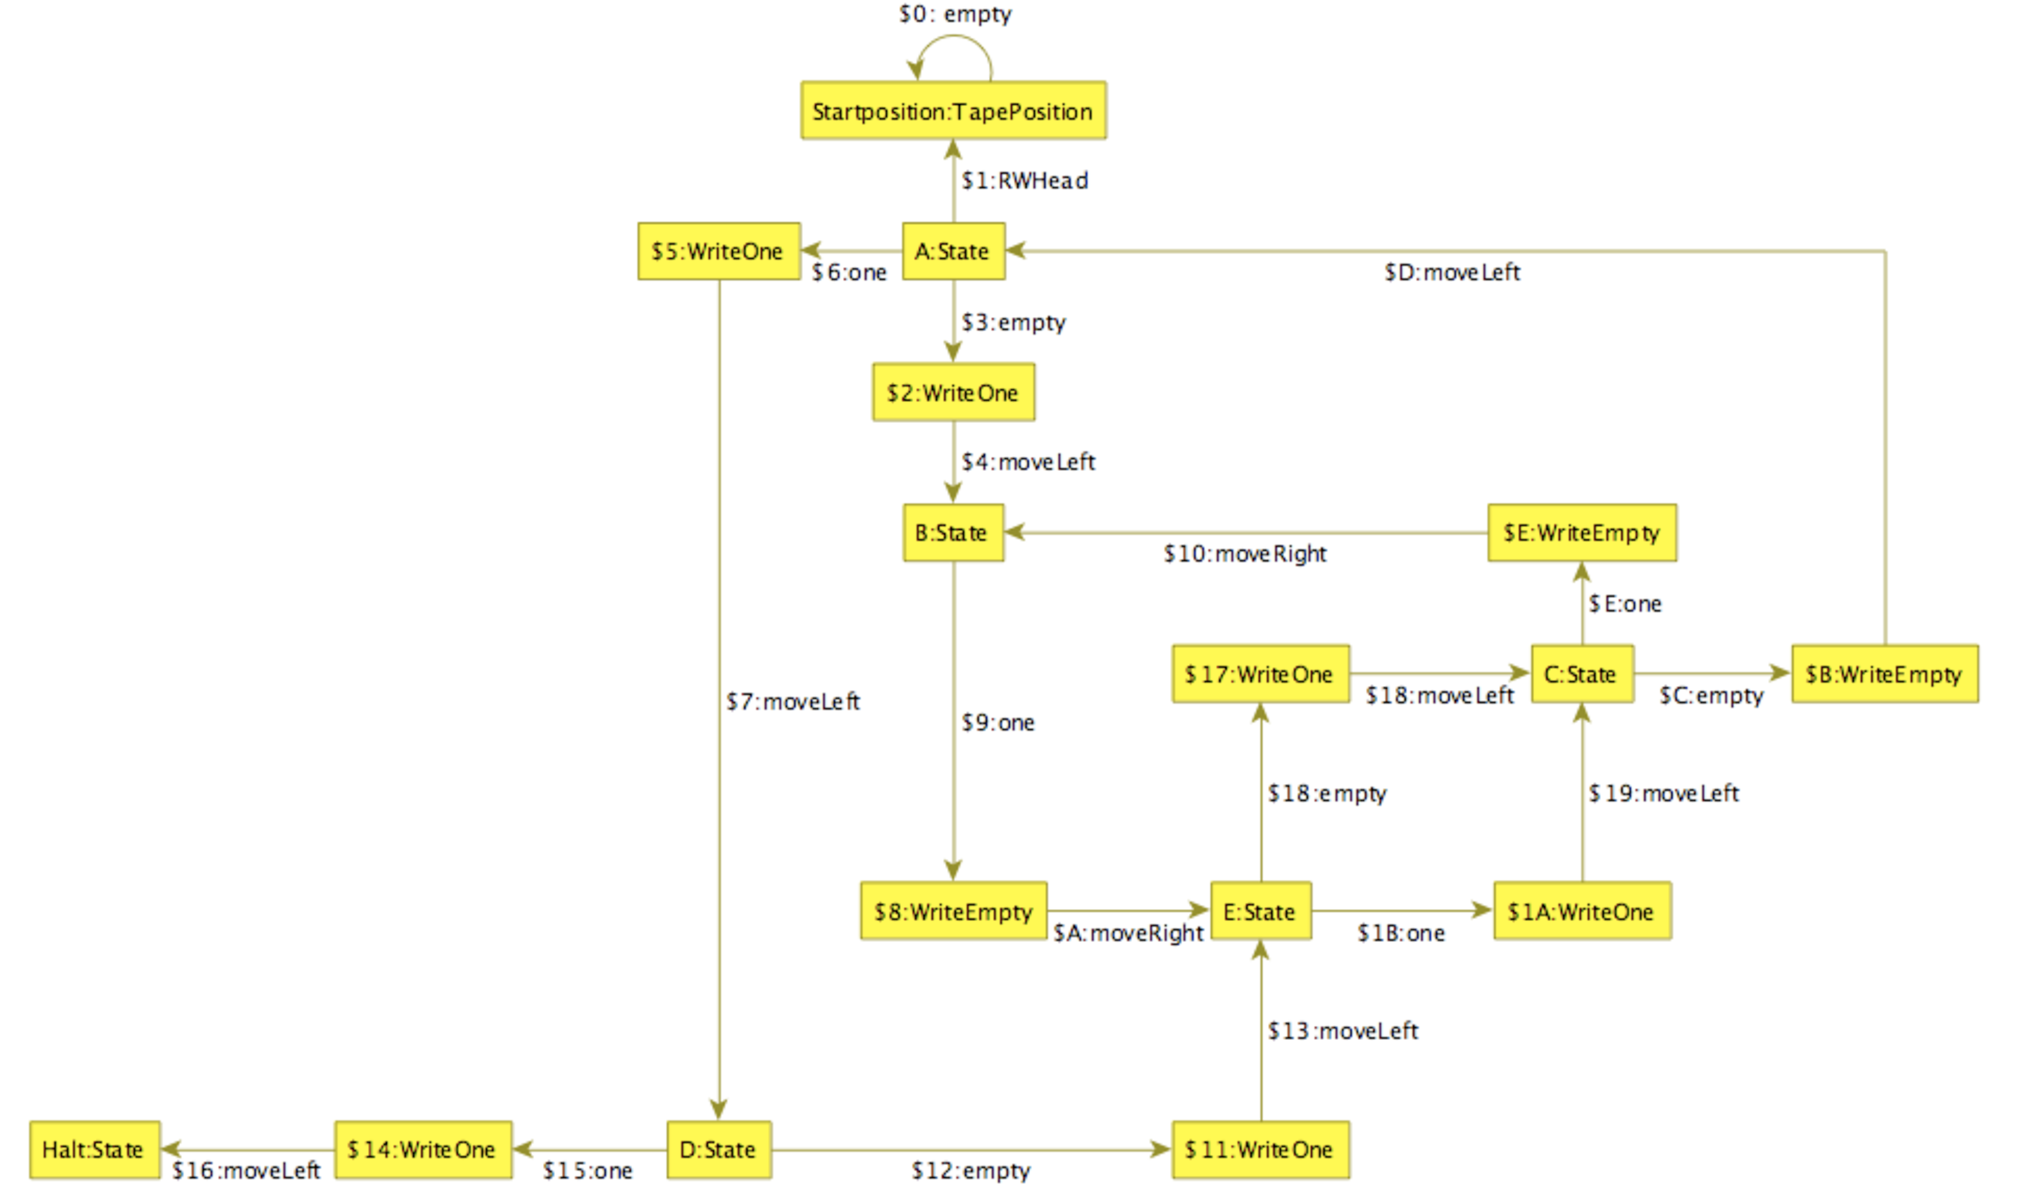
\includegraphics[width=\linewidth-2\fboxsep-2\fboxrule]{fig/bbstart}}
\end{center}

We have an initial host graph now. The graph rewrite sequence is quite straight forward and generic to the Turing graph model. Note that for each state the ``\texttt{\dots Empty\dots} | \texttt{\dots One\dots}'' selection is unambiguous.
%\pagebreak %HACK
\begin{grshell}[firstnumber=last]
  xgrs ((readOneRule | readEmptyRule) & (writeOneRule | writeEmptyRule) & (ensureMoveLeftValidRule | ensureMoveRightValidRule) & (moveLeftRule | moveRightRule))[32]

\end{grshell}
\quad\\We interrupt the machine after 32 iterations and look at the result so far:
\begin{center}
  \fbox{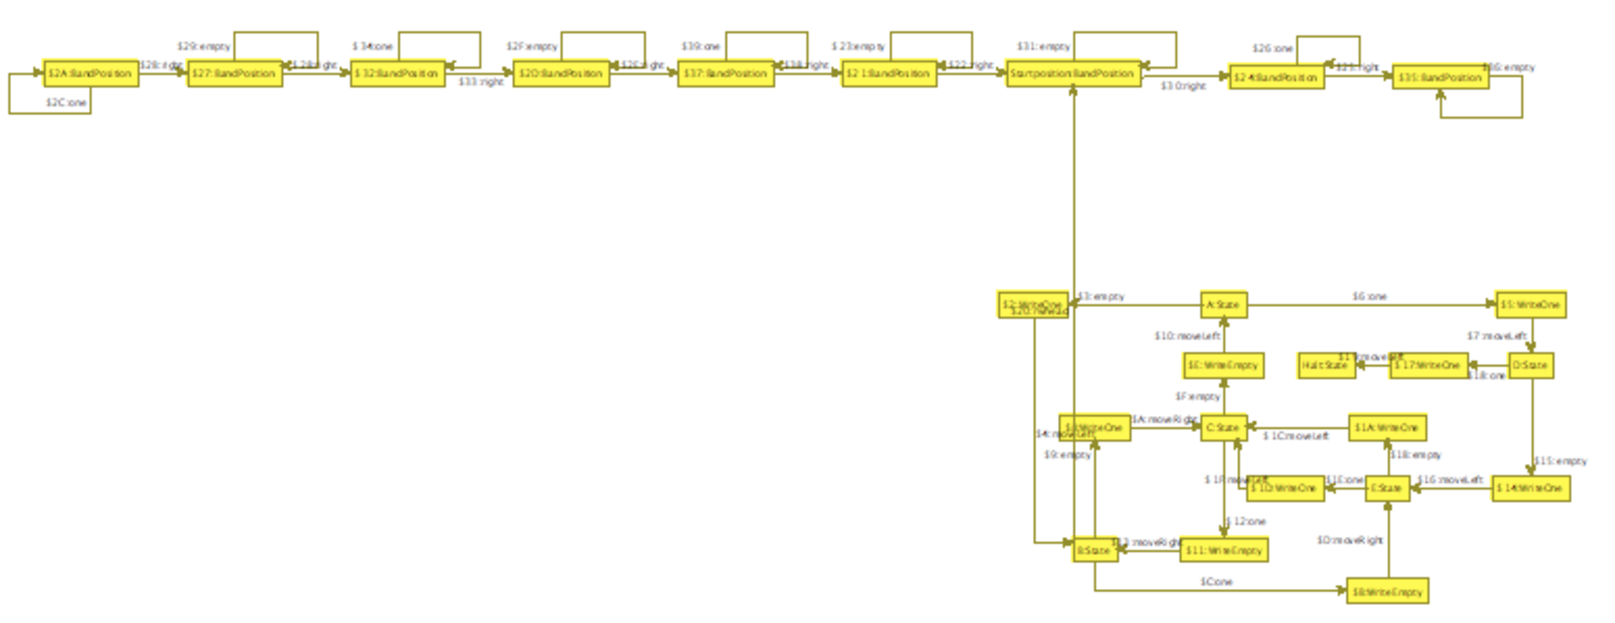
\includegraphics[width=\linewidth-2\fboxsep-2\fboxrule]{fig/bbmiddle}}
\end{center}
In order to improve the performance we generate better \indexed{search plan}s. This is a crucial step for execution time: With the initial search plans the beaver runs for 1 minute and 30 seconds. With improved search plans after the first 32 steps he takes about 8.5 seconds\footnote{On a Pentium 4, 3.2Ghz, with 2GiB RAM.}.
\begin{grshell}[firstnumber=last]
custom graph analyze_graph
custom actions gen_searchplan readOneRule readEmptyRule writeOneRule writeEmptyRule ensureMoveLeftValidRule ensureMoveRightValidRule moveLeftRule moveRightRule

\end{grshell}

Let the beaver run:
\begin{grshell}[firstnumber=last]
  xgrs ((readOneRule | readEmptyRule) & (writeOneRule | writeEmptyRule) & (ensureMoveLeftValidRule | ensureMoveRightValidRule) & (moveLeftRule | moveRightRule))*
\end{grshell}




\thebibliography{99}
\bibitem{geiss} R. Geiß et al.: \emph{\GrG: A Fast SPO-Based Graph Rewriting Tool} in Graph Transformations, number 4178 in LNCS, pages 383-397, Springer, 2006
\bibitem{kroll} M. Kroll: \emph{Portierung des C-Anteils des Graphersetzungssystems \GrG\ nach C\# mit Erweiterungen}, Studienarbeit, Fakultät für Informatik, Universität Karlsruhe, 2007
\bibitem{hack} S. Hack: \emph{Graphersetzung für Optimierung in der Codeerzeugung} Diplomarbeit, Fakultät für Informatik, Universität Karlsruhe, 2003
\bibitem{grund} D. Grund: \emph{Negative Anwendungsbedingungen für den Graphersetzer \GrG} Studienarbeit, Fakultät für Informatik, Universität Karlsruhe, 2004 
\bibitem{adam} A. Szalkowski: \emph{Negative Anwendungsbedingungen für das suchprogrammbasierte Backend von GrGen} Studienarbeit, Fakultät für Informatik, Universität Karlsruhe, 2005
\bibitem{batz} G. Batz: \emph{Graphersetzung für eine Zwischendarstellung im Übersetzerbau} Diplomarbeit, Fakultät für Informatik, Universität Karlsruhe, 2005
\bibitem{pascal} K. Jensen, N. Wirth: \emph{Pascal User Manual and Report} Springer, $^41991$
\bibitem{isoc} \emph{Programming languages -- C}, ISO/IEC 9899:1999, 2005
\bibitem{bb} A. Dewdney: \emph{A computer trap for the Busy Beaver, the hardest-working machine} Scientific American, 251
(2), pages 10-12, 16, 17, August 1984
\bibitem{beaver} H. Marxen, J. Buntrock: \emph{Old list of record TMs.}\\ http://www.drb.insel.de/~heiner/BB/index.html. Version: August 2000

\end{document}
 
